%************************************************
\chapter[Application du modèle à l'analyse sensorielle]{Application du modèle morphologique à l'analyse sensorielle des scènes sonores environnementales urbaines}\label{ch:psycho_xp}
%************************************************

\gl{TODO: concernant le titre: pourquoi modèle morphologique plus que "simulateur" ? il manque le coté "création" dans modèle morphologique}

\section{Introduction}

Comme nous l'avons vu (\cf~Section~\ref{sec:ch3_contribSource}), la recherche sur les paysages sonores a besoin d'outils permettant d'analyser les influences séparées des différentes sources sur les qualités affectives de l'environnement. La simulation offre des possibilités intéressantes (\cf~Section~\ref{sec:ch4_anaSo}), car elle nous permet d'obtenir des scènes sonores dont nous connaissons tous les paramètres structuraux, en particulier les caractéristiques distinctes des différentes sources. 
 
Afin de montrer les potentialités inhérentes à l'utilisation de scènes simulées en analyse sensorielle, nous choisissons, comme cadre applicatif, le problème de l'agrément perçu dans les environnements sonores urbains. 

Cette section présente les résultats d'une série de quatre expériences visant, chacune, à comprendre comment les différentes sources sonores qui composent une scène influent sur la perception de l'agrément. Toutes ses expériences s'appuient sur la simulation. La première est l'expérience de simulation à proprement parler, \ie~où les sujets doivent créer les environnements. Les autres sont des épreuves de notation ou de tri classiques, utilisant les scènes simulées comme stimuli:

\begin{enumerate}
\item \emph{expérience de simulation}: au cours de cette expérience, chaque sujet doit simuler deux environnements sonores urbains, le premier idéal/agréable et le deuxième non-idéal/désagréable, en utilisant l'outil et le protocole de simulation décrits à la section~\ref{sec:ch4_simscene};
\item \emph{évaluation de l'agrément}: les sujets doivent évaluer l'agrément des scènes simulées à partir d'une échelle sémantique;
\item \emph{évaluation de l'agrément après modification des scènes}: comme pour l'expérience précédente, les sujets doivent évaluer l'agrément des scènes simulées à partir d'une échelle sémantique. Cependant les scènes ont été modifiées, \ie~privées de certaines classes de sons identifiées comme ayant un impact sur l'agrément perçu; 
\item \emph{catégorisation libre}: les sujets doivent catégoriser les scènes sonores simulées. Au delà du problème initial de l'agrément, cette dernière expérience nous amène à considérer logiquement l'influence de la composition sémantique des scènes sur les jugements de similarités.
\end{enumerate}

Les expériences 1 et 2 vont de pair, et sont toutes deux décrites dans la section~\ref{sec:xp1_2}. Les expériences 3 et 4 sont, elles, décrites respectivement dans les sections~\ref{sec:xp3} et~\ref{sec:xp4}  \\

Tout au long de la présentation de ces expériences et de leurs résultats, nous poursuivrons deux objectifs:

\begin{itemize}
\item \emph{objectif méthodologique}: montrer les possibilités offertes par l'utilisation de scènes simulées dont nous connaissons précisément la partition (\cf~Section~\ref{sec:ch4_modelDes}) dans le cadre d'études sensorielles ayant trait à la perception des sons;
\item \emph{objectif applicatif}: étudier quels sont les éléments qui participent à la perception de l'agrément dans les environnements sonores urbains. 
\end{itemize}

\section[Agrément perçu et composition sémantique]{L'impact de la composition sémantique des scènes sur la perception de l'agrément}
\label{sec:xp1_2}

\subsection{Objectif}

L'objectif est d'étudier les influences spécifiques des différentes sources sonores qui composent les environnements urbains, sur la perception de l'agrément, en utilisant la simulation. Pour ce faire, nous planifions nos deux premières expériences (\cf~Figure~\ref{fig:xp1_2}):

\begin{itemize}
\item \emph{expérience de simulation}: comme précisé auparavant, au cours de cette expérience, les sujets simulent les environnements qui serviront de stimuli pour les étapes suivantes. Chaque sujet compose deux scènes opposées, les premières répondant à la description idéales/agréables (i-scènes), les secondes répondant à la description non idéales/désagréables. Cette épreuve de simulation a fait l'objet d'une expérience pilote \citep{lafay2013atiam,lafay2014new}; \gl{TODO: préciser xp pilote}
\item \emph{expérience d'évaluation}: a l'issue de la simulation, nous n'avons, de fait, qu'une connaissance binaire des propriétés affectives des scènes simulées: idéale (i) et non-idéale (ni). Cette seconde étape a pour but d'affiner notre connaissance sur l'agrément de chacune des scènes. Pour ce faire, nous demandons à un deuxième groupe de sujets d'évaluer, à partir d'une échelle sémantique, l'agrément de chacune des scènes simulées. L'expérience d'évaluation sert deux buts:
\begin{enumerate}
\item évaluer l'influence des différentes sources sur l'agrément perçu, de manière séparée, pour chaque type d'environnement (i ou ni);
\item détecter la présence de cas extrêmes ou ambigus (\emph{outlier}) dans les scènes simulées. Pour le reste de notre étude, les qualités hédoniques imposées (i et ni) servent de référence, de vérité terrain. Il nous faut donc garantir qu'il n'y ait pas d’ambiguïté entre les cas extrêmes des i- et ni-scènes, \ie~que la note d'agrément la plus basse des i-scènes reste supérieure à la note la plus haute des ni-scènes.
\end{enumerate}

\end{itemize}

Notre analyse s'appuie sur les données produites par les deux expériences.

\begin{figure}[t]
        \myfloatalign
        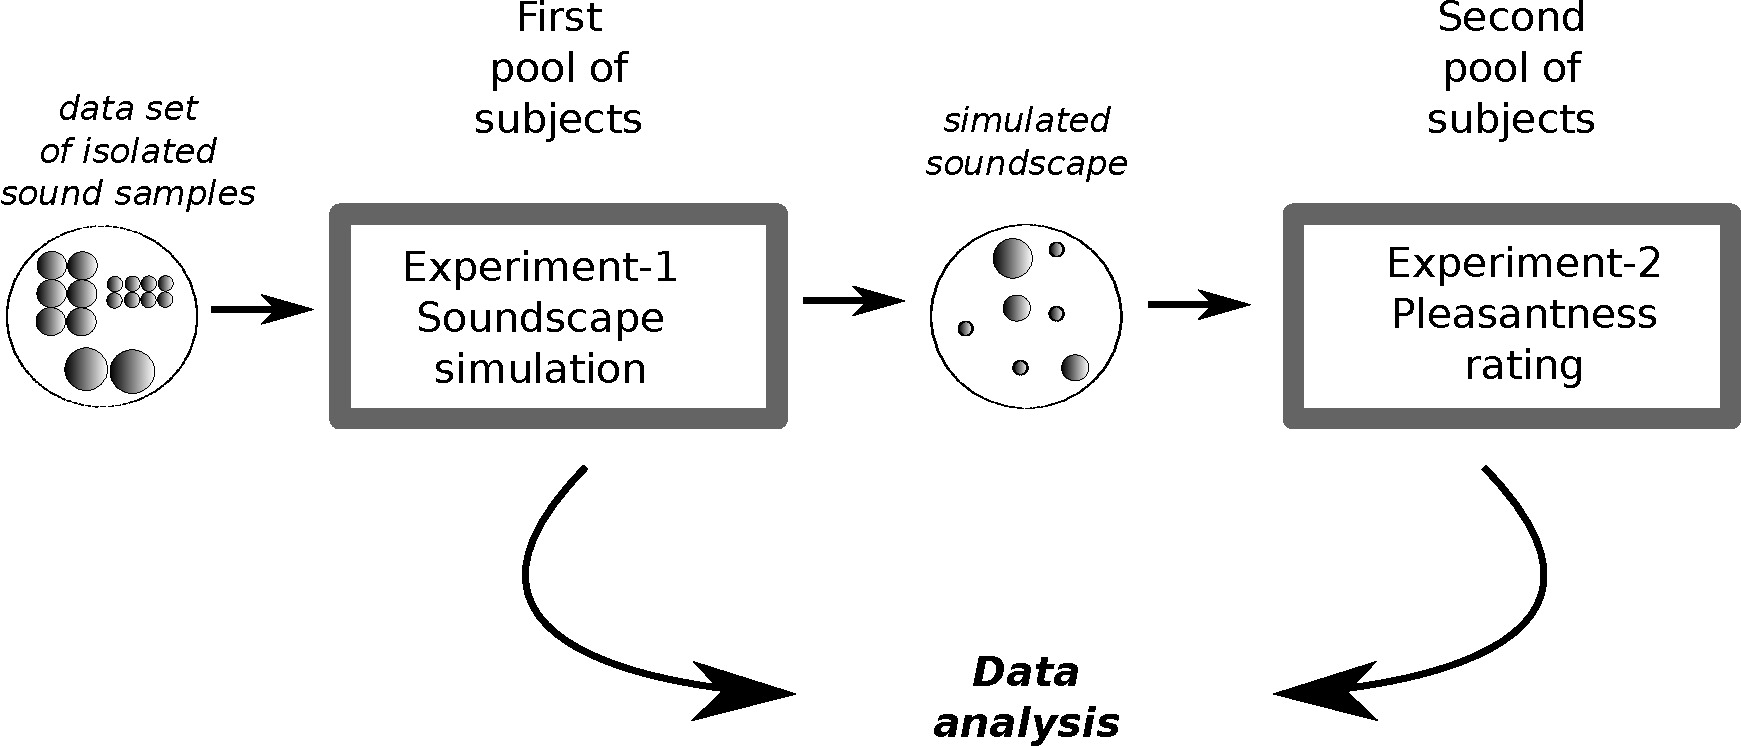
\includegraphics[width=.8\linewidth]{gfx/5}
        \caption{Planification expérimentale des éxperiences de simulation et d'évaluation de l'agrément}\label{fig:xp1_2}
\end{figure}



\subsection{Banque de données de sons isolés}

Dans cette section, nous présentons les processus de sélection et d'acquisition des sons utilisés comme matériau de base lors de la simulation des environnements sonores urbains. La banque de données est identique à celle utilisée dans le cadre de l'expérience pilote \citep{lafay2013atiam,lafay2014new}. 

Pour plus de détails sur l'organisation interne de la banque de données, ainsi que sur l'interface graphique permettant de sélectionner ces dernières, se référer aux sections~\ref{sec:ch4_dbEventTexture} et~\ref{sec:ch4_ssf}.

\subsection{Typologie des sources sonores présentes dans l'environnement urbain}

Afin de créer un corpus de sons isolés de référence pour la simulation, nous avons réalisé une typologie des sons environnementaux urbains. 

Pour ce faire, une étude bibliographique est effectuée, afin d'identifier les sources et ambiances sonores les plus souvent citées dans la littérature. Cette étude porte sur 16 articles ou thèses. Chacun d'eux traite de la manière dont nous discriminons les paysages sonores urbains. Il ressort que plusieurs approches sont possibles :

\begin{itemize}
\item 9 articles abordent le problème par une approche perceptive, soit en identifiant ou répertoriant des catégories de sources sonores, soit en étudiant l'impact de classes de sons spécifiques sur la perception de l'environnement : \cite{maffiolo_caracterisation_1999,raimbault2002simulation,guastavino_etude_2003,defreville2004aactivity,raimbault2005urban,dubois2006cognitive,devergie_relations_2006,guastavino2006ideal,niessen2010categories}
\item 3 articles proposent une classification morpho-typologique, divisant l’environnement sonore urbain en ``\,zones sonores\,'' possédant une identité acoustique forte, selon la configuration et la pratique du site : \cite{maffiolo_caracterisation_1999,beaumont2004pertinence,polack2008perceptive}
\item 2 articles répertorient et classifient les sources sonores d’un point de vue expert : \cite{leobon_analyse_1986,brown2011towards}
\end{itemize}

La nature des classes est établie par rapport aux catégories perceptives, ou classes de sons, les plus souvent citées dans ces publications. À partir des éléments relevés, nous établissons deux taxonomies : une pour les événements (\cf~Figure~\ref{fig:taxonomie}.a), une autre pour les textures (\cf~Figure~\ref{fig:taxonomie}.b). Comme évoqué à la section~\ref{sec:db_ui}, la structure taxonomique de ces deux ensembles s'inspire grandement de l'axe vertical de l'organisation catégorielle proposée par E. Rosch (\cf~Section~\ref{sec:ch3_categoEtAbstract}), \ie~plus le niveau d'abstraction de la classe est élevé, plus la description de la classe est précise, et plus les sources sonores incluses dans cette classe sont semblables (\cf~Figure~\ref{fig:orgDb}). Pour les événements, nous considérons quatre niveaux d'abstraction allant des classes les plus globalisantes (niveau d'abstraction 0), aux classes les plus spécifiques (niveau d'abstraction 3). Pour les textures, nous ne considérons que trois niveaux d'abstraction.

Pour les événements, les regroupements se font en grande majorité par rapport à la source, et sont d’ordre sémantique. Pour les textures, nous considérons également la nature des lieux hébergeant ces dernières (\eg~\emph{parc}, \emph{rue}). La typologie des classes d'événements suit la nomenclature source-action introduite à la section (\cf~Section~\ref{sec:ch4_sourceAction}). En ce sens, elle est très similaire à cette autre typologie de sources sonores urbaines, effectuée postérieurement \citep{Salamon14}.

\begin{figure}[t]
        \myfloatalign
        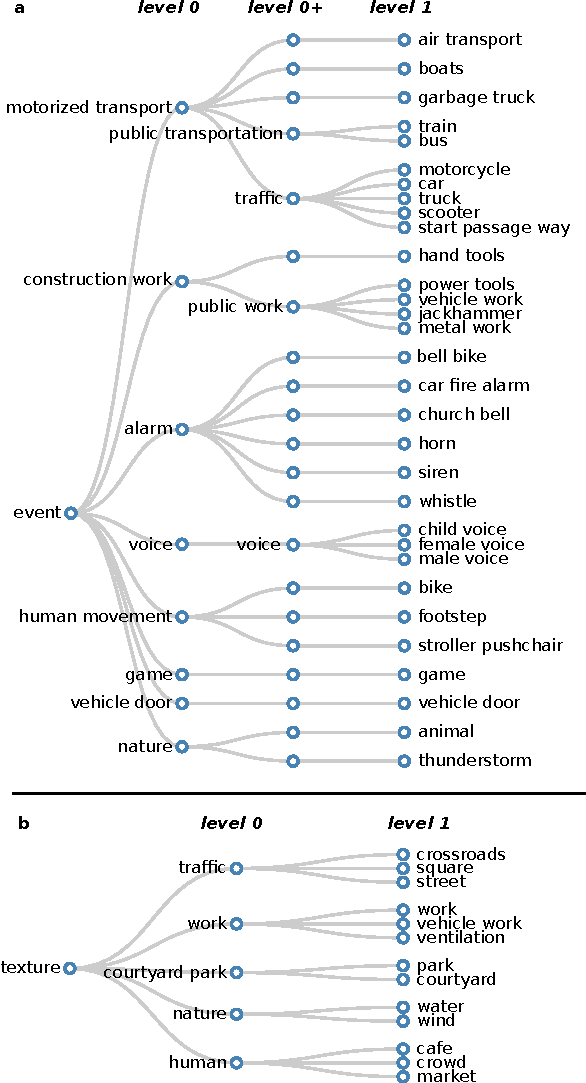
\includegraphics[width=.5\linewidth]{gfxHierarchy/taxonomy}
       \caption[Taxonomies des classes de sons utilisées pour la simulation des environnements sonores urbains]{Taxonomies des classes de sons utilisées pour la simulation des environnements sonores urbains pour (a) les événements sonores, et (b) les textures sonores. Nous présentons ici uniquement les niveaux d'abstraction 0 et 1. Un niveau intermédiare, nommé $0+$, et utilisé pour l'analyse, est également introduit.}\label{fig:taxonomie}
\end{figure}

\subsection{Acquisition des sons isolés}
\label{sec:ch5_recordDataSet}

Sur la base des typologies précédemment établies, 483 sons ont été collectés, dont 381 événements, et 102 textures.

Parmi les événements :

\begin{itemize}
\item 260 sont issus d’enregistrements effectués pour l'étude;
\item 89 sont issus de la banque de sons \emph{SoundIdeas}\footnote{Pour plus de détails sur \emph{SoundIdeas} voir :\url{ http://www.sound-ideas.com/}};
\item 32 sont issus de la banque de sons \emph{Universal SoundBank}\footnote{Pour plus de détails sur \emph{Universal SoundBank} voir : \url{http://www.universal-soundbank.com/}}.
\end{itemize}

Parmi les textures:

\begin{itemize}
\item 72 sont issues d’enregistrements effectués pour l'étude;
\item 23 sont issues de la banque de sons \emph{SoundIdeas};
\item 7 sont issues de la banque de sons \emph{Universal SoundBank}.
\end{itemize}

Tous les enregistrements ont été effectués à l’aide d'un micro canon \emph{AT8035}\footnote{\cf~\url{http://eu.audio-technica.com/fr/products/product.asp?catID=1&subID=6&prodID=1845}} relié à un enregistreur \emph{ZOOM H4n}\footnote{\cf~\url{http://www.zoom.co.jp/english/products/h4n/}}. L’utilisation du micro canon nous permet d’isoler les événements sonores du brouhaha urbain. Pour les textures, il nous permet d’éviter les événements sonores proches du preneur de son. Nous pouvons ainsi pointer des "zones sonores", en nous tenant à une certaine distance de ces dernières, afin de capter uniquement le brouhaha émanant de la zone ciblée.

Tous les sons ont été normalisés au même niveau $RMS$ \footnote{Le niveau $RMS$, de l'anglais \emph{Root Mean Square} qui désigne la valeur efficace d'un signal. Formellement, le niveau $RMS$ $x_{RMS}$ d'un signal $x=(x_1,x_2,\ldots,x_n)$ s'obtient en calculant la moyenne quadratique de ce dernier $x_{RMS}=\sqrt{\dfrac{1}{n}\sum\limits_{i} x_i^2}$} de $-12$ $dB$ (FS) \footnote{$dB$ (FS) est le sigle anglais désignant une valeur en décibels relative à la pleine échelle (\emph{relative to Full Scale}), \ie~le rapport entre le niveau du signal et sa valeur maximale. Dans notre cas, ce niveau pleine échelle est de 1 Volt.}.

\subsection{Planification expérimentale}

\subsubsection{Épreuve de simulation}
\label{sec:ch5_planExpSimu}

Nous nommons cette expérience: \emph{expérience 1.a}. \\

\textbf{Procédure} \\

Les sujets doivent simuler deux environnements sonores urbains, chacune des scènes devant durer 1 minute. Pour ces simulations, les sujets doivent se conformer aux consignes suivantes:

\begin{itemize}
\item première simulation : simuler un paysage sonore \textbf{urbain plausible} qui, selon vous, est idéal (où vous aimeriez vivre);
\item deuxième simulation : simuler un paysage sonore \textbf{urbain plausible} qui, selon vous, est non-idéal (où vous n'aimeriez pas vivre).
\end{itemize}

Tous les sujets commencent par simuler l'environnement idéal. Les sujets ne prennent connaissance de la deuxième consigne qu'à la fin de la première simulation.

Les sujets son totalement libres dans le choix des sons, et des paramètres (pour plus de détails sur les paramètres se référer à la section~\ref{sec:ch4_param}). Ils doivent cependant se soumettre à deux contraintes:

\begin{itemize}
\item le sujet doit prendre le point de vue d’un auditeur fixe;

\item le paysage sonore doit être réaliste, au sens de physiquement plausible. Autrement dit, le sujet à tout à fait le droit de placer 10 chiens dans son paysage sonore, mais il n’a pas le droit de placer un chien aboyant toutes les 10 millisecondes.

\end{itemize}

Ces contraintes font partie de la consigne. Aucun contrôle n'est fait \emph{a priori} dans l'interface de simulation.

Chaque processus de simulation comprend deux parties :

\begin{enumerate}
\item la réalisation de la simulation: cette étape peut, elle même, se décomposer en trois actions (\cf~Section~\ref{sec:ch4_processSimu}):
\begin{itemize}
\item sélectionner les classes de sons
\item nommer les classes de sons sélectionnées
\item paramétrer les pistes (\cf~Section~\ref{sec:ch4_seqSample}) relatives aux classes de sons sélectionnées
\end{itemize}
\item la réalisation d'un commentaire libre du paysage sonore simulé
\end{enumerate}

En complément, et une fois les deux scènes sonores réalisées, les sujets sont invités à:

\begin{itemize}
\item indiquer les sources sonores qu'ils voulaient mettre, mais qu'ils n'ont pas trouvées;
\item commenter l’ergonomie du logiciel de simulation;
\item commenter l’ergonomie de l'interface de sélection.
\end{itemize}

Avant de commencer la première simulation, un tutoriel de 20 minutes est proposé aux sujets, afin qu'ils se familiarisent avec le logiciel de simulation, et la banque de données. Le tableau~\ref{tab:indSimu} résume les étapes de l’expérience, ainsi que leurs durées respectives. L'expérience est prévue pour durer 2h30. \\

\begin{table}[t]
\centering
\begin{tabular}{c c c} 
Index          & Tâche                               & Durée (min) \\                      
\hline
1 & Présentation de l'expérience                     & 10 \\
  & Lecture de la consigne                           &  \\
\hline
2 & Tutoriel (Réalisation d'une scène test)          & 20 \\
\hline
3 & Première simulation: scène idéale                & 40 \\
\hline
4  & Commentaire de la scène idéale                  & 15 \\
\hline
3 & Deuxième simulation: scène non-idéale            & 40  \\
\hline
4  & Commentaire de la scène non-idéale              & 15 \\
\hline
5 & Critique de l'interface de simulation            & 10 \\
  & et de l'interface de sélection                   & \\
\hline
\end{tabular}
\vspace{0.5mm}
\caption{Résumé des étapes de l’expérience de simulation}
\label{tab:indSimu}
\end{table}

\textbf{Apparatus} \\

Tous les sujets passent l'expérience sur des machines identiques (\gl{description des machines}). L'audio est diffusé en stéréophonie, par le biais de casques audio. Pendant le tutoriel, les sujets doivent ajuster le niveau sonore à un volume confortable. Ils ne peuvent le modifier par la suite.

Tous les sujets réalisent l'expérience simultanément. Ils sont répartis de manière égale dans trois pièces identiques, toutes possédant un environnement calme. Ils n'ont pas le droit de s'adresser la parole pendant l'expérience.

Trois expérimentateurs, un dans chaque pièce, sont présents durant la totalité de l'expérience, afin de contrôler le bon déroulement de cette dernière, et de répondre aux éventuelles questions des sujets.  \\

\textbf{Participants} \\

44 étudiants (14 femmes) de L’École Centrale de Nantes ont participé à l'expérience. Ils ont tous sensiblement le même âge (moyenne: 21.6, écart-type: 2). Tous les sujets sont Nantais, et vivent dans cette ville depuis deux ans ou plus.

Sur les 44 sujets, 40 réalisent l'expérience avec succès, produisant au final 80 scènes sonores simulées, dont 40 scènes idéales, et 40 scènes non idéales. 4 sont éliminés pour non respect et/ou incompréhension des consignes, d'une part, dépassement du temps, d'autre part.



\subsubsection{Épreuve d'évaluation de l'agrément}
\label{sec:ch5_planExpEvaA}

Nous nommons cette expérience: \emph{expérience 1.b}. \\

\textbf{Procédure} \\

En raison de contraintes temporelles, les sujets n'évaluent que des séquences de 30 secondes des scènes simulées, chacune de ces séquences commençant à la seconde 15, et finissant à le seconde 45, de la scène évaluée.

L'évaluation s'effectue sur une échelle sémantique bipolaire de 7 points, allant de -3 (non-idéale/très désagréable) à +3 (idéale/très agréable). Avant de noter une scène, les sujets doivent obligatoirement écouter les 20 premières secondes de cette dernière. Après la notation, ils sont libres de passer à la scène suivante.

Pour chaque sujet, les scènes sont présentées dans un ordre aléatoire. Les 10 premières scènes permettent au sujet de calibrer ses notes. Elles sont obligatoirement composées de 5 scènes idéales et de 5 non-idéales. Ces 10 premières scènes sont rejouées à la fin de l'expérience, et seules les notes données à la deuxième occurrence sont prises en compte. 

L'expérience est prévue pour durer 30 minutes. Les sujets ne connaissent pas la nature des scènes.\\

\textbf{Apparatus} \\

Tous les sujets passent l'expérience sur des machines identiques (\gl{description des machines}). L'audio est diffusé en stéréophonie, par le biais de casques audio semi-ouvert \emph{Beyer-Dynamic DT 990 Pro}. Toutes les scènes sonores ont été re-simulées sur la base des partitions obtenues lors de l'expérience de simulation. Le niveau sonore de sortie est identique pour tous les sujets.

Tous les sujets réalisent l'expérience simultanément, dans un environnement calme. Ils n'ont pas le droit de s'adresser la parole pendant l'expérience. 

Un expérimentateur est présent durant la totalité de l'expérience, afin de contrôler le bon déroulement de cette dernière, et de répondre aux éventuelles questions des sujets.  \\

\textbf{Participants} \\

10 étudiants (2 femmes) de L’École Centrale de Nantes ont participé à l'expérience. Aucun d'entre eux n'a réalisé l'expérience de simulation. Tous les sujets ont sensiblement le même âge (moyenne: 23.1, écart-type: 1.8). Tous les sujets sont Nantais, et vivent dans cette ville depuis deux ans ou plus.

Tous les sujets ont réalisé l'expérience avec succès.

\subsection{Données et méthodes d'analyses}

\subsubsection{Nature des données analysées}
\label{sec:ch5_dataType1}

A partir des données produites par l'épreuve de simulation, nous analysons:

\begin{itemize}
\item les partitions des scènes simulées;
\item les signaux des scènes simulées;
\item les commentaires sur les sons manquants, et l'ergonomie des interfaces de simulation et de sélection.
\end{itemize}

Chaque scène est décrite par un groupe de descripteurs. C'est sur la base de ces descripteurs que nous pratiquons l'analyse. Un résumé des descripteurs, ainsi que des acronymes les désignant, est présenté dans le Tableau~\ref{tab:acronyme}. Afin de rester cohérent avec l'épreuve d'évaluation, les descripteurs issus des partitions, ou des signaux des scènes, ne sont pas calculés sur la durée totale de celles-ci, mais sur une version réduite de 30 secondes (\cf~Section~\ref{sec:ch5_planExpEvaA}). 

Pour chaque scène sonore, trois types de descripteurs sont considérés:

\begin{itemize}
\item \emph{perceptif}: il s'agit de l'agrément perçu de la scène simulée, évalué sur une échelle sémantique 7 points. Nous notons $\mathcal{A}_{scene}$ l'agrément moyen d'une scène, obtenu en moyennant les notes de tous les sujets. De même, nous notons  $\mathcal{A}_{sujet}$ l'agrément par sujet, en moyennant l'ensemble de ses notes. Compte tenu du faible nombre de sujets, nous faisons le choix, dans cette étude, de ne pas normaliser les notes d'agrément;
\item \emph{sémantique}: il s'agit d'un vecteur booléen noté $S=(x_1,x_2,\ldots,x_n)$, indiquant les classes de sons présentes dans la scène. Chaque point $x$ de ce vecteur correspond à une classe de sons particulière: $x=1$ si la classe est présente dans la scène, et $x=0$ autrement. La dimension $n$ des vecteurs dépend du niveau d'abstraction considéré, \eg~pour le niveau d'abstraction 1, qui comprend $44$ classes de sons, cette dimension sera de $n=44$.
\item \emph{structurel}: Les descripteurs structurels sont calculés à partir des partitions et des signaux des scènes simulées. Trois descripteurs structurels sont envisagés:
\begin{itemize}
\item \emph{diversité} ($DIV$) : il s'agit d'un scalaire représentant la diversité des classes sonores utilisées pour simuler une scène. Nous calculons $DIV$ en comptant le nombre de classes de sons distinctes utilisées pour une simulation. Ce nombre dépend du niveau d'abstraction considéré. Par exemple, considérant les deux sous classes du niveau d'abstraction 2 \emph{passage de voiture} et \emph{démarrage de voiture}, toutes deux appartenant à la classe \emph{voiture} du niveau d'abstraction 1, nous comptons deux classes pour la diversité des niveaux d'abstraction 2, et 1, et seulement 1, pour les niveaux d'abstraction 0 et 1;
\item \emph{densité} ($D$) : il s'agit d'un scalaire représentant le nombre de sources sonores présentes en moyenne. Pour obtenir $D$, nous calculons le logarithme du nombre d'éléments sonores par fenêtre de 125 millisecondes (sans recouvrement), et moyennons au cours du temps. Le calcul de $D$ peut inclure toutes les sources sonores de la scène, ou seulement une partie. Dans ce cas, les fenêtres ne contenant pas de sources sonores ne sont pas prises en compte. Nous notons $D(E)$ et $D(T)$ les densités calculées en considérant séparément les sources d'événements et de textures sonores;
\item \emph{niveau Sonore} ($L$) : pour représenter le niveau sonore, nous nous inspirons de la mesure $L_{Aeq}$. Dans notre cas, il s'agit d'un scalaire, calculé sur le signal en volts, et non en pression, et donné en décibels, en prenant un référentiel de 1 Volt. Le niveau est obtenu en calculant, toutes les secondes, la moyenne quadratique du signal, et en moyennant sur la durée de la scène. Un filtrage de type A est opéré avant le calcul des moyennes quadratiques. D'autre descripteurs, inspirés eux aussi de descripteurs acoustiques classiques ($L_{Amin}$, $L_{Amax}$, $L_{A10-90}$), et utilisant un opérateur autre que la moyenne (minimum, maximum, les 10-90ème quantiles) pour intégrer les fenêtres de 1 seconde, ont été testés. Mais, ces derniers présentant tous une corrélation élevée avec $L$ ($r_{pearson}\geq0.76$, $p<0.01$), nous conservons le scalaire ci-devant mentionné comme unique descripteur objectif du niveau sonore.
\end{itemize}
\end{itemize}

\begin{table}[t]
\centering
\begin{tabular}{c c c c c} 
Descripteurs          & Acronymes   &   & Descripteurs            & Acronymes  \\                       
\cline{1-2} \cline{4-5}
Densité               & $D$         &   & Diversité               & $DIV$    \\
                      &             &   &                         &          \\
Densité               & $D(E)$      &   & Diversité               & $DIV(E)$ \\
(événements)          &             &   & (événements)            &          \\
Niveau                & $L$         &   & Diversité               & $DIV(T)$ \\
                      &             &   & (textures)              &          \\
Niveau                & $L(E)$      &   & Agrément moyen          & $\mathcal{A}_{scene}$     \\
(événements)          &             &   & (par scène)             &         \\
Niveau                & $L(T)$      &   & Agrément moyen          & $\mathcal{A}_{sujet}$        \\
(textures)            &             &   & (par sujet)             &      \\
                      &             &   &                         &      \\
\multicolumn{3}{c}{Termes} &  \multicolumn{2}{c}{Acronymes} \\ 
\hline
\multicolumn{3}{c}{Idéal/agréable}                 & \multicolumn{2}{c}{i}       \\
\multicolumn{3}{c}{non-idéale/désagréable}         & \multicolumn{2}{c}{ni}      \\
\multicolumn{3}{c}{Scène idéale/agréable}          & \multicolumn{2}{c}{i-scène} \\
\multicolumn{3}{c}{Scène non-idéale/désagréable}   & \multicolumn{2}{c}{ni-scène} \\
\hline
\end{tabular}
\vspace{0.5mm}
\caption{TODO}
\label{tab:acronyme}
\end{table}

\subsubsection{Méthodologie et Outils statistiques}
\label{sec:ch5_methodoEtStat1}

Afin d'évaluer l'impact spécifique des différentes sources sonores sur l'agrément perçu, nous soumettons nos travaux aux 6 tests/études de significativité présentés ci-après:

\begin{itemize}
\item \emph{étude qualitative} : afin de vérifier la validité écologique de 1) la banque de données et 2) l'interface de sélection, nous réalisons une étude qualitative des critiques ergonomiques effectuées par les sujets;
\item \emph{étude comparative entre les descripteurs structurels} : afin d'évaluer si la distinction affective imposée entre les i- et ni-scènes impacte de manière significative la nature des scènes, \ie~s'il existe des différences significatives entre les descripteurs structurels et/ou l'agrément perçu, nous évaluons cette significativité à partir d'un test de Student à deux échantillons appariés (\cf~Annexe~\ref{app:student});
\item \emph{étude de l'influence des descripteurs structurels sur l'agrément perçu}: afin d'évaluer l'impact potentiel des descripteurs structurels sur l'agrément perçu, nous étudions l'existence de corrélations linéaires entre ces deux types de descripteurs. Pour mesurer la corrélation, nous utilisons le coefficient de Pearson (\cf~Annexe~\ref{app:corr}). Nous adoptons ici une méthodologie couramment utilisée dans l'approche dimensionnelle;
\item \emph{étude comparative entre les descripteurs sémantiques}: afin d'apprécier si la distinction affective imposée a eu un impact sur la composition des scènes en terme de sources sonores, ou, pour être plus précis, s'il existe des classes de sons qui ont été particulièrement utilisées pour simuler un type d'environnement, nous utilisons le V-test. Nous vérifions si la présence d'une classe de sons est typique d'un environnement (i ou ni). Le test est effectué pour chaque niveau d'abstraction, et séparément, pour les classes d'événements et de textures. Pour chaque classe $j$ et chaque type d'environnements $k$ ($k={i,ni}$), la valeur $V_{jk}$ du V-test se calcule comme suit: 

\begin{equation*}
V_{jk}=\dfrac{c_{jk}-c_k\frac{c_j}{c}}{\sqrt{c_k\frac{c-c_k}{c-1}\frac{c_j}{c}(1-\frac{c_j}{c})}}
\end{equation*}

où $c$ est le nombre de classes utilisées, $c_k$ le nombre de classes utilisées pour un type d'environnements $k$, $c_j$ le nombre de classes $j$ utilisées, et $c_{jk}$ le nombre de classes $j$ utilisées pour un type d'environnements $k$. Le V-test teste l'hypothèse nulle que la proportion $\frac{c_{jk}}{c}$ ne diffère pas significativement de la proportion $\frac{c_{jk}}{c_k}$. Si pour un environnement $k$, et une classe $j$, l'hypothèse est rejetée, la classe $j$ est alors typique de l'environnement $k$. Les classes typiques sont nommées \textbf{marqueurs sonores};

\item \emph{étude des espaces de représentations induits par les descripteurs sémantiques}: afin d'étudier si une représentation basée uniquement sur la présence ou l'absence des classes de sons permet de séparer les deux types d'environnements, nous considérons l'espace induit par les descripteurs sémantiques $S$. $S$ étant un vecteur booléen, nous calculons les distances entre les scènes à partir de la distance de Hamming. Considérant les deux vecteurs $S_1=(x_{1,1},x_{1,2},\ldots,x_{1,n})$, et $S_2=(x_{2,1},x_{2,2},\ldots,x_{2,n})$ de dimension $n$, avec $x={0,1}$, la distance de Hamming $d_{ham}$ mesure le pourcentage de coordonnées qui diffèrent entre les deux vecteurs:   


\begin{equation*}
d_{ham}(S_1,S_2)=\dfrac{1}{n}\sum_{i=1}^{n} (x_{1,i} \bigoplus x_{2,i})
\end{equation*}

où $\bigoplus$ désigne l'opérateur du \emph{ou-exclusif}. plus la composition des deux scènes est similaire, et plus ces deux scènes sont proches. L'utilisation de la distance de Hamming permet de prendre en compte de manière égale les classes présentes et absentes. Pour mesurer la capacité intrinsèque de l'espace à séparer les i- et ni-scènes, nous utilisons une métrique de \emph{clustering} nommée précision au rang $k$ ($P@k$). La $P@k$ mesure la précision obtenue après que $k$ items ont été retrouvés. Formellement, pour chaque scène $s_i$, nous calculons le rapport entre le nombre de scènes $s_j$, prises parmi les $k$ plus proches voisines de $s_i$, et  partageant le même label que $s_i$, sur le nombre d'items à retrouver ($k$). La $P@k$ est alors la moyenne des rapports pour tous les items;

\item \emph{étude de l'influence spécifique des marqueurs sonores sur l'agrément perçu}: afin d'évaluer les contributions spécifiques de certaines sources sonores, nous évaluons une nouvelle fois l'impact potentiel des descripteurs structurels sur l'agrément perçu, mais en ne tenant compte, cette fois, que des marqueurs sonores pour calculer ces descripteurs.
\end{itemize}

Excepté le V-test, tous les tests de significativité sont effectués avec un seuil critique $\alpha=0.05$. Pour le V-test, étant donné que nous testons beaucoup de classes, une correction de Bonferroni (\cf~Annexe~\ref{app:statuni}) est appliquée. Pour les valeurs $p$, dans le cas où la valeur $p\geq0.05$, nous indiquons sa valeur. Dans le cas ou $0.01\leq p<0.05$, nous indiquons seulement $p<0.05$. Dans le dernier cas nous indiquons $p<0.01$.

Concernant l'interprétation du coefficient de corrélation de Pearson adoptée dans ce document, nous invitons le lecteur à se référer à l'annexe~\ref{app:corr}.

\subsection{Validité écologique de l'expérience}

\subsubsection{Diversité de la banque de sons}

Nous voulons vérifier que la diversité des classes de sons proposées est suffisante pour pouvoir simuler un environnent sonore. Nous analysons les commentaires des sujets sur la banque de données. 63\% d'entre eux indiquent avoir été, au moins une fois, dans l'incapacité de trouver un son, avec un maximum de 4 sons par sujet. Parmi les sons manquants relevés, nous identifions 26 classes de sons dont:

\begin{itemize}
\item 16 sont bien présentes dans la banque de données, l'incapacité des sujets à les trouver n'étant donc pas imputable à la diversité de la base.
\item 1 fait référence à des sons de musique, que nous avons choisi délibérément d'occulter. \gl{TODO discuter avant}
\item 9 sont effectivement absentes.  
\end{itemize}

Concernant ces dernières, nous observons qu'il s'agit de classes très spécifiques (\eg~\emph{voiture de sport} ou \emph{voix d'adolescent}), et qui peuvent être remplacées par des classes similaires (\eg~\emph{voiture}, \emph{voix d'enfant} ou \emph{voix d'adulte}). Nous en concluons que la diversité proposée par la banque de sons est satisfaisante et suffisante dans le cadre de notre étude.

\subsubsection{Ergonomie de l'interface de sélection}

Nous voulons vérifier l'efficience de l'interface de sélection. Nous analysons les retours des sujets. $32.5\%$ d'entre eux indiquent spontanément que l'interface est un moyen ``\,simple et efficace\,'' de sélectionner des sons sans l'aide de texte. $57.5\%$ ne font pas mention de difficultés particulières, $10\%$ signalent enfin avoir rencontré des difficultés avec l'interface, sans toutefois que la simulation en ait été affectée.

Nous en concluons que l'interface de sélection, sans texte, ne perturbe pas les sujets outre mesure. Un même constat avait été tiré de l'expérience pilote \citep{lafay2013atiam,lafay2014new}. \\

\gl{TODO: vérifier une dernière fois}

\subsubsection{Ergonomie de l'interface de simulation}

\subsection{Vérification de l'agrément des scènes simulées}

Nous analysons ici l'agrément perçu des $80$ scènes sonores simulées. La Figure~\ref{fig:xp2_Aa} affiche l'agrément moyen $\mathcal{A}_{scene}$ pour les i- et ni-scènes. 

Dans un premier temps, et afin de garantir la cohérence de nos données, nous voulons nous assurer qu'aucune ni-scène n'ait un $\mathcal{A}_{scene}$ supérieur à celui d'une i-scène. Quatre des scènes ne respectent pas la contrainte. Elles et leurs correspondantes i ou ni sont retirées. 36 i-scènes et 36 ni-scènes restent dans le champ de l'analyse.

Dans un deuxième temps, nous voulons tester si les sujets ont bien perçu une différence d'agrément entre les i- et ni-scènes. Pour ce faire, nous observons l'agrément moyen de chaque sujet $\mathcal{A}_{sujet}$, calculé séparément, pour chaque type d'environnement (\cf~Figure~\ref{fig:xp2_Ab}). Il apparaît que les i-scènes ont bien été perçues comme significativement plus agréables ($p<0.01$) que les ni-scènes.

\begin{figure}[t]
        \myfloatalign
        \subfloat[]
        {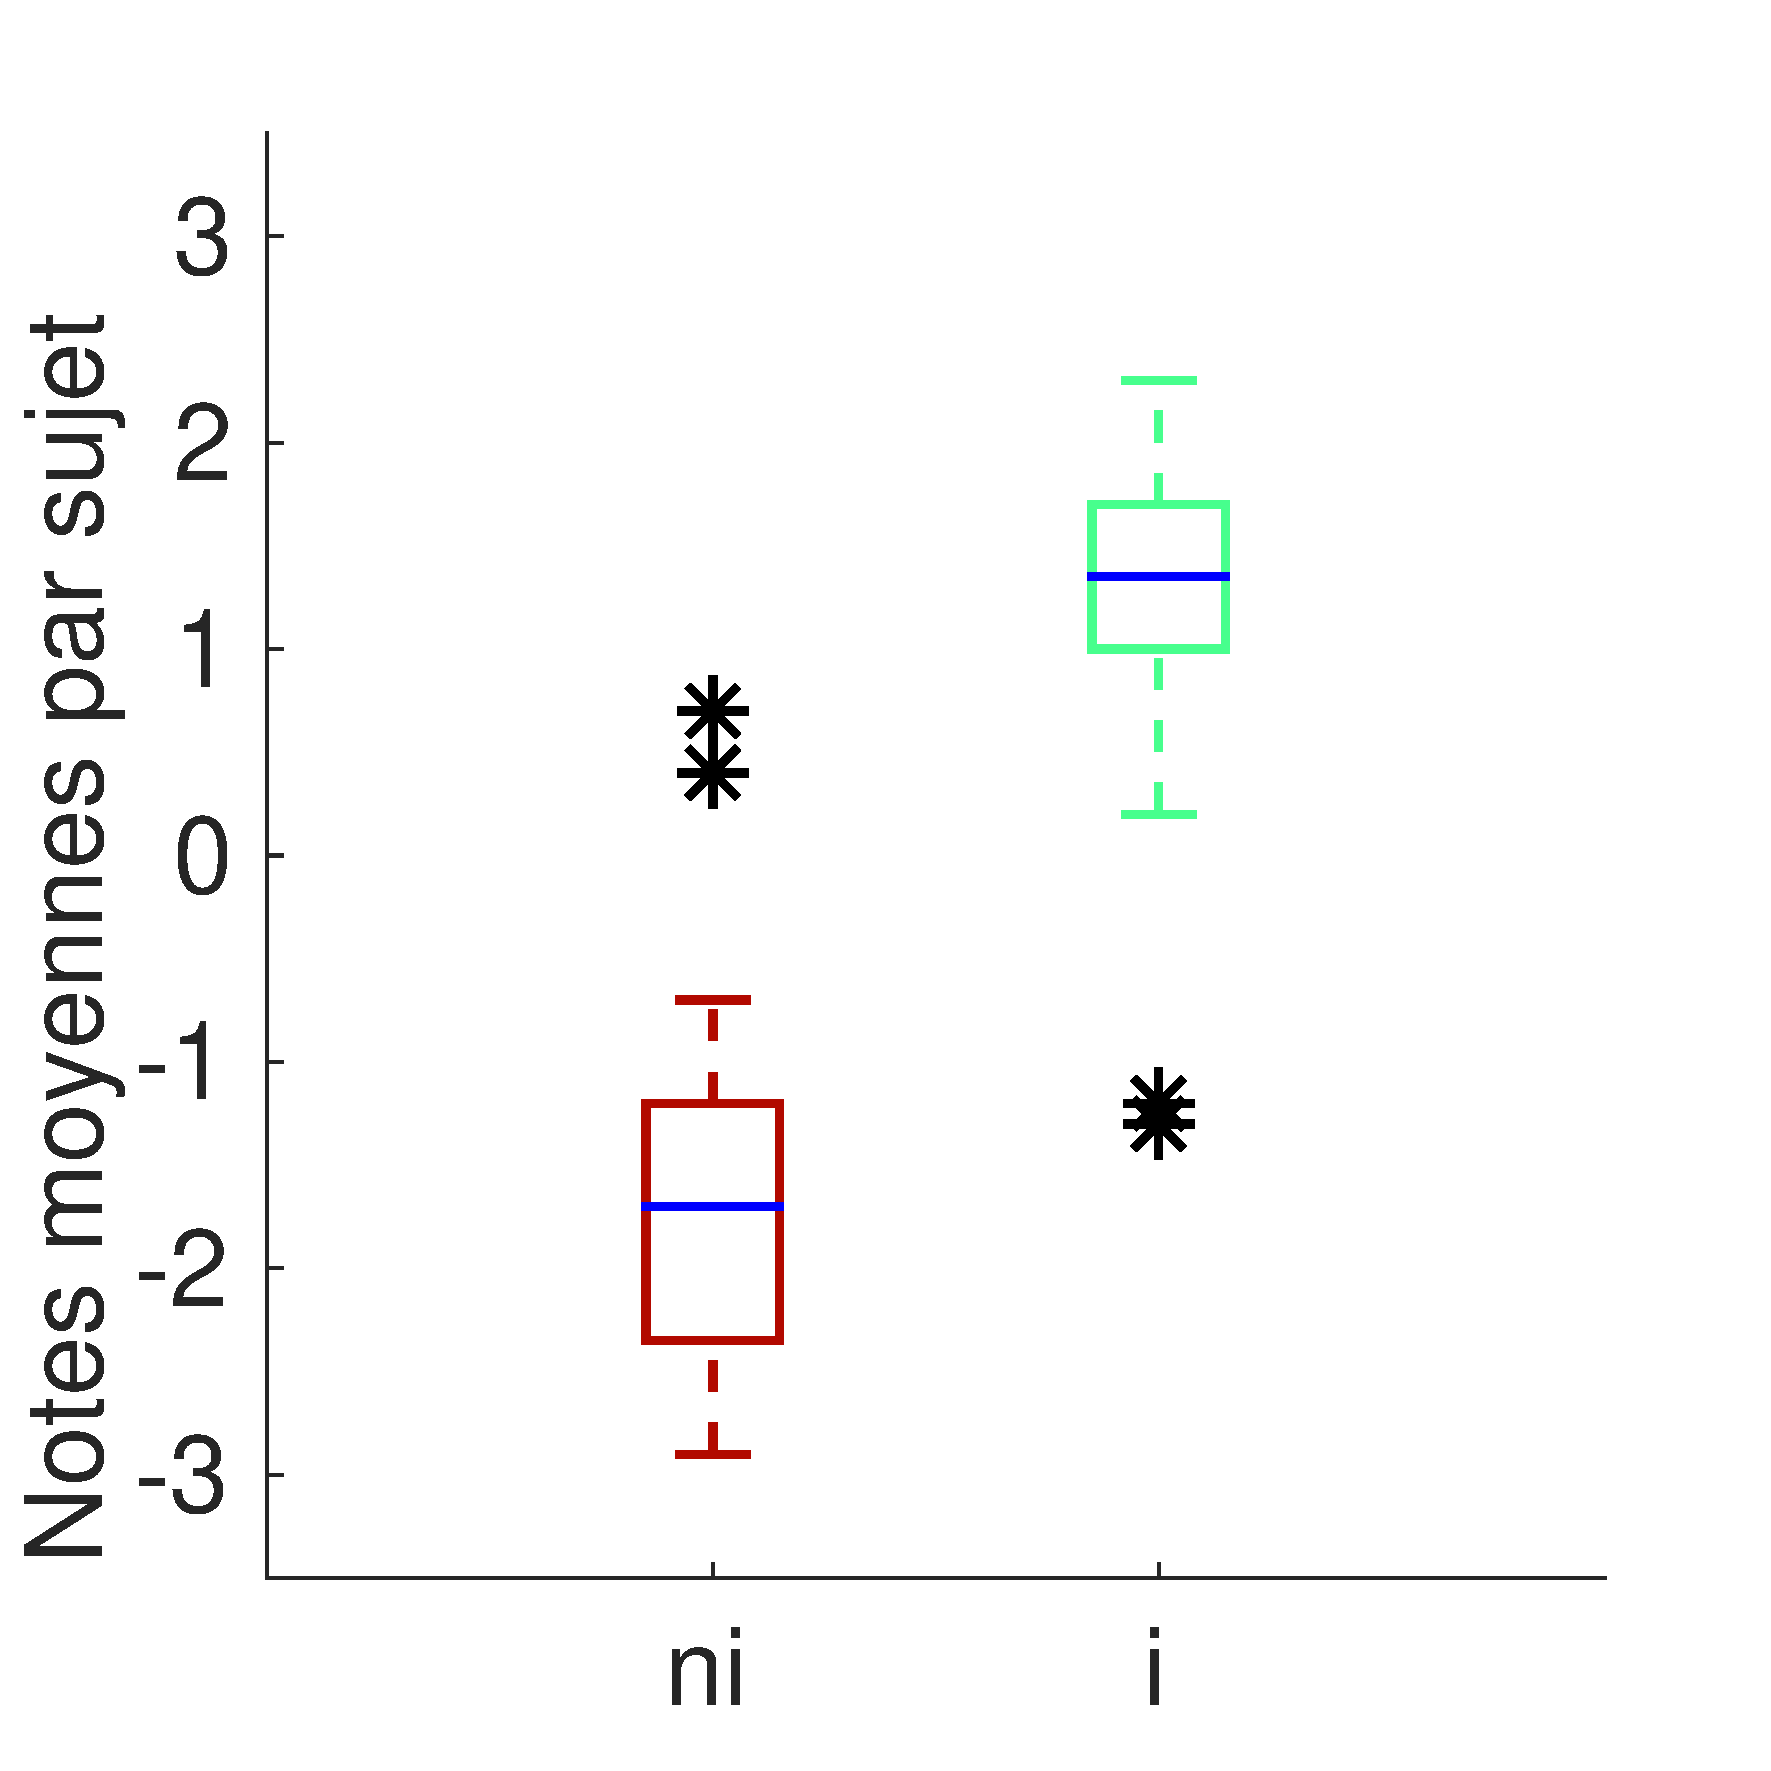
\includegraphics[width=.4\linewidth]{gfxXpUrbanSoundscape/xp2_1}\label{fig:xp2_Aa}}
        \subfloat[]
        {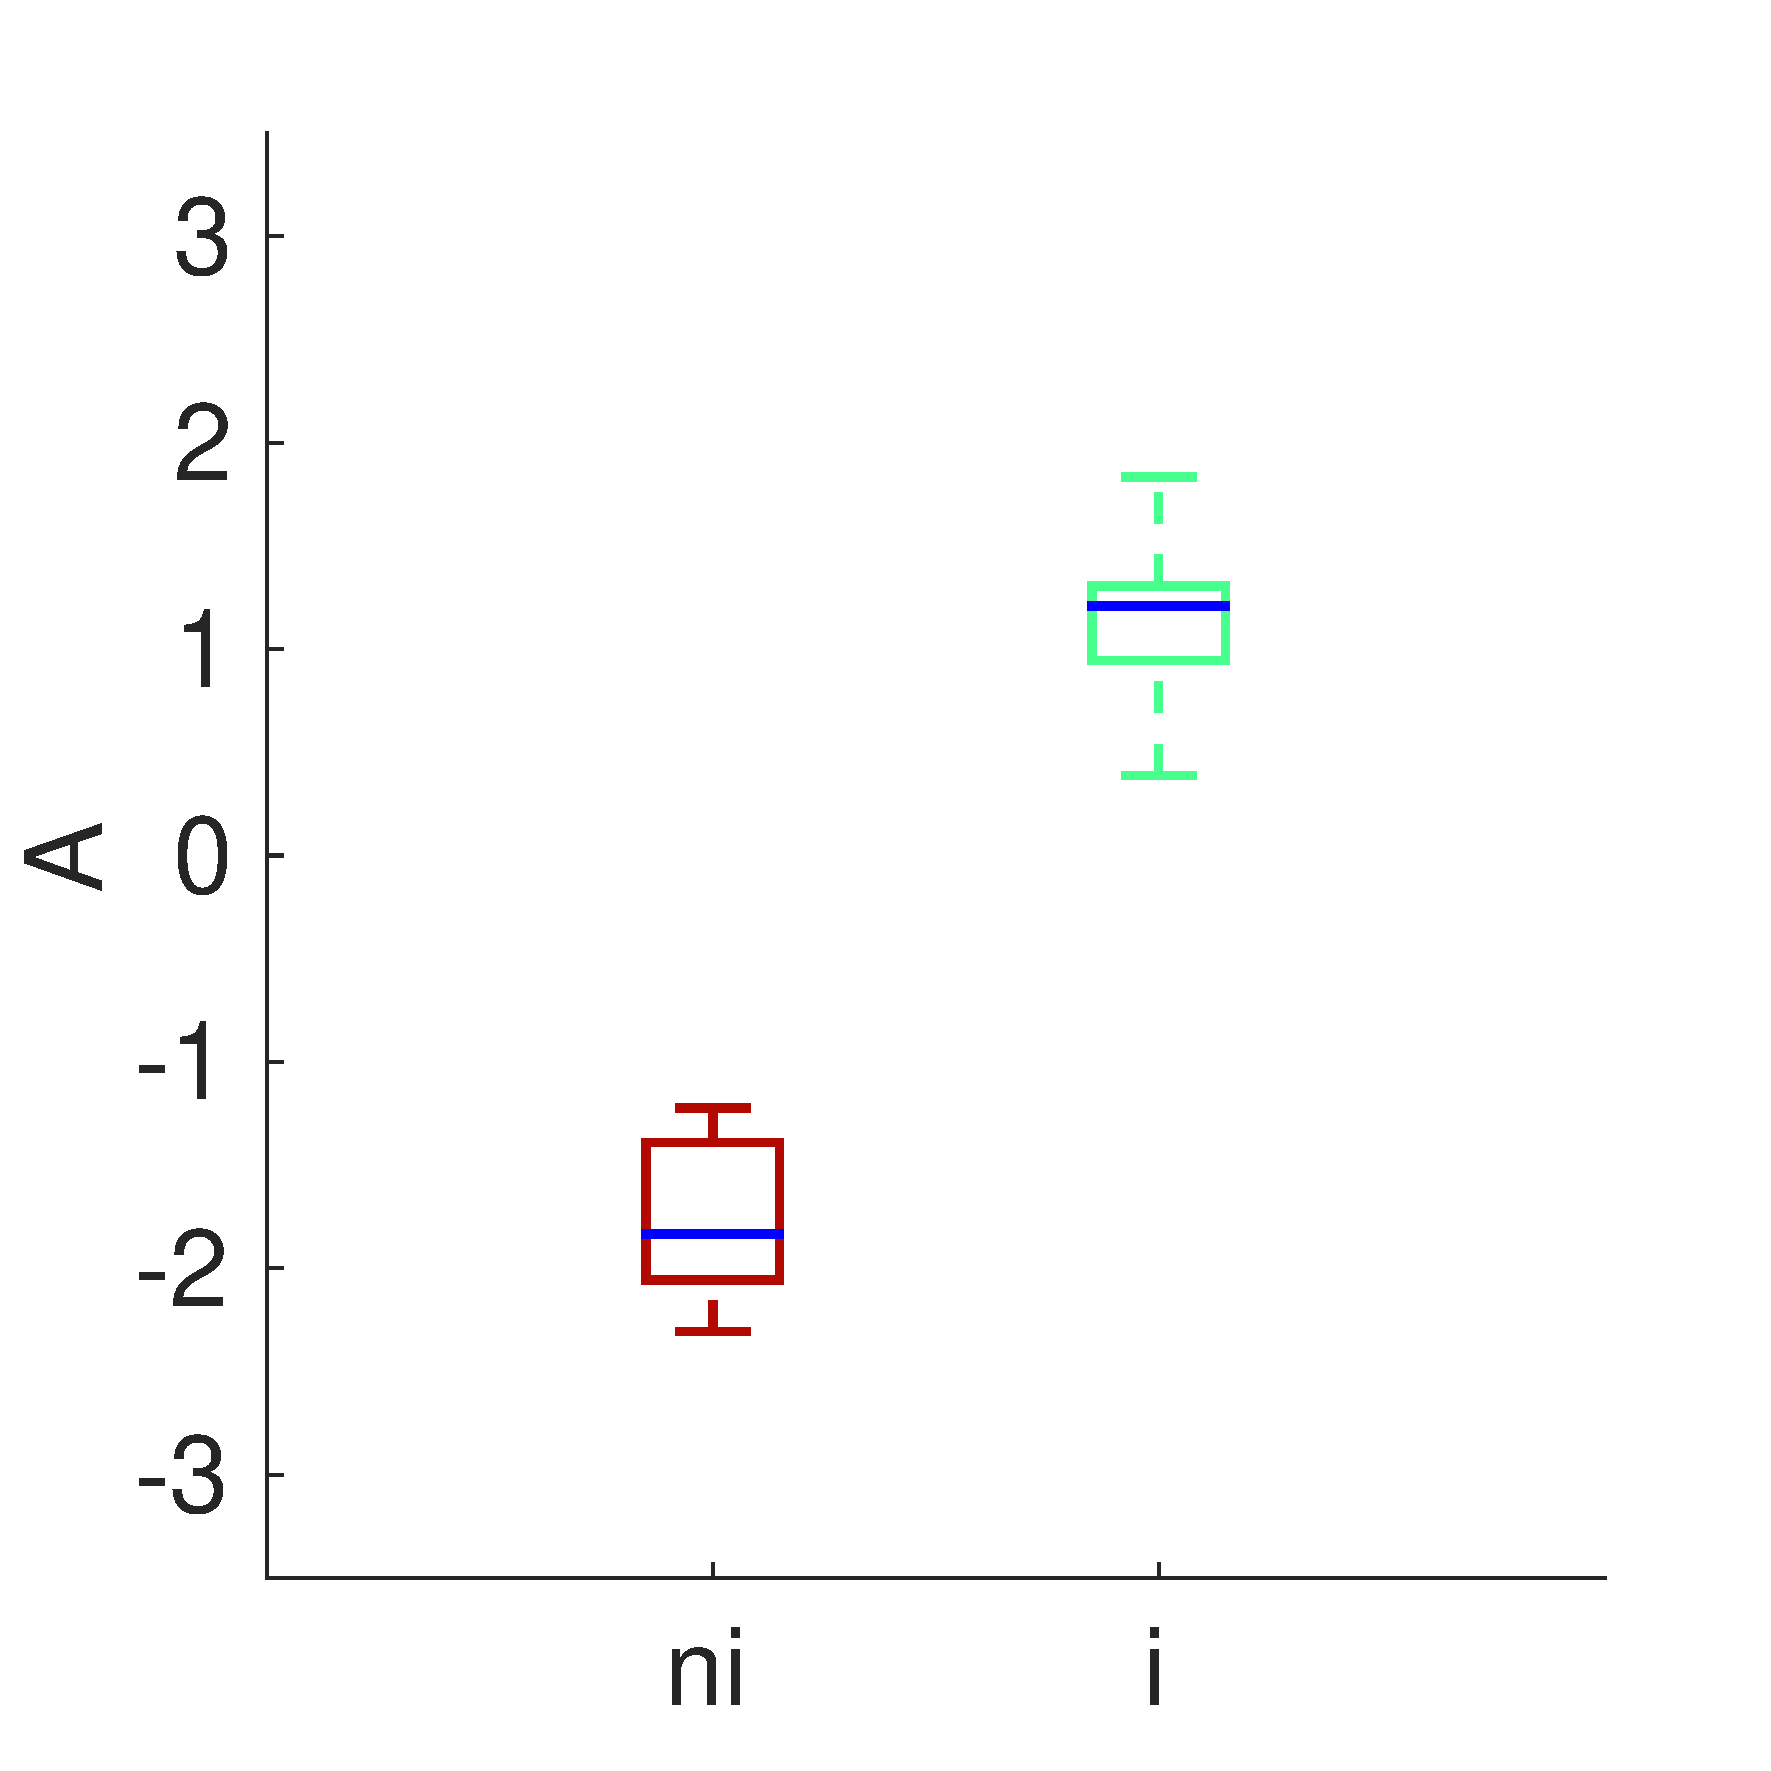
\includegraphics[width=.4\linewidth]{gfxXpUrbanSoundscape/xp2_2}\label{fig:xp2_Ab}}
       \caption[TODO]{TODO}\label{fig:xp2_A}
\end{figure}
 
\subsection{Étude comparative entre les descripteurs structurels}

En premier lieu, nous nous concentrons sur le niveau sonore. Les figures~\ref{fig:soundlevela},~\ref{fig:soundlevelb} et~\ref{fig:soundlevelc} affichent les distributions des niveaux $L$, $L(E)$ et $L(T)$. Il existe bien une différence de niveau  significative entre les i- et ni-scènes ($L$: $p<0.01$), avec un écart moyen de -7 $dB$. Cette différence affecte aussi bien les événements ($L(E)$: $p<0.01$, écart moyen: -7 $dB$) que les textures ($L(T)$: $p<0.01$, écart moyen: -6 $dB$). 

Nous vérifions, sans surprise, que le niveau des sources sonores est bien un indicateur d'agrément, les ni-scènes ayant tendance à être plus fortes, \gl{fait reporté dans un grand nombre d'études} \gl{TODO: citation}. Nous constatons encore que cette différence de niveaux s'observe de manière égale pour les événements et les textures sonores. 

Il apparaît que ce sont les événements qui impactent le plus le niveau global des scènes, l'écart entre $L$ et $L(E)$ n'étant que de 1 $dB$ pour les i-scènes et les ni-scènes. Cette observation fait écho aux résultats obtenus par Kuwano~\al \citep{kuwano_memory_2003}. Au cours de leur expérience, les auteurs demandent à leurs sujets d'évaluer une série d'environnements sonores, d'abord, de manière globale, ensuite, d'en évaluer le niveau aux instants où chacun identifie une source sonore. L'étude montre qu'il n'y a pas de différences significatives entre les jugements globaux et les moyennes des jugements instantanés. Pour en revenir à notre expérience, c'est comme si nos sujets avaient inconsciemment tenu compte de cette réalité perceptive lors de la simulation, en faisant porter le niveau sonore global par des sons courts et bien identifiés, \ie~les événements.

Nous observons, enfin, que le niveau seul ne permet pas de clairement faire la distinction entre les différents types d'environnements. En effet, $20\%$ des i-scènes ont un niveau supérieur au niveau minimal des ni-scènes, alors qu'il n'y a pas de recouvrement, si l'on considère l'agrément perçu $\mathcal{A}_{scene}$.

En second lieu, nous nous penchons sur les densités de sources sonores. Les Figures~\ref{fig:densitya} et~\ref{fig:densityb} affichent les distributions de $D$ et $D(E)$. Que l'on prenne en compte toutes les sources, ou uniquement les événements, la densité est significativement plus élevée pour les ni-scènes ($D$: $p<0.01$, $D(E)$: $p<0.01$). Nous observons un écart moyen de $+0.36$ pour $D$ (soit en moyenne 2.3 sources sonores par fenêtre de plus pour les ni-scènes), et de $+0.32$ pour $D(E)$ (soit en moyenne 2.1 sources sonores par fenêtre de plus pour les ni-scènes). Si ces écarts sont très similaires, c'est que la densité des textures $D(T)$ ne varie pas de manière significative entre les i- et ni-scènes ($D(T)$: $p<0.08$), l'écart moyen étant de $+0.17$ (soit en moyenne 0.7 sources sonores par fenêtre de plus pour les ni-scènes), et l'écart médian étant, quant à lui, nul.

Nous constatons ici que la densité peut être un indicateur de qualité, si l'on considère uniquement les événements sonores. Comme pour les niveaux sonores, la densité ne permet pas de clairement séparer les i- et ni-scènes,  $43\%$ des i-scènes ayant un $D(E)$ supérieur à la densité d'événement minimale des ni-scènes.

En dernier lieu, nous nous intéressons à la diversité. Nous affichons sur la figure~\ref{fig:diversity} $DIV(E)$ et $DiV(T)$, en séparant les différents niveaux d'abstractions. Excepté pour le niveau d'abstraction 0, la diversité de classes d'événements sonores est plus élevée pour les ni-scènes ($DIV(E)$ niveaux 1,2 et 3: $p<0.01$ ), avec en moyenne 2 classes présentes en plus. Aucune différence significative n'est observée pour les textures.

Les tendances globales observées montrent, d'une part, qu'un environnement sonore non-idéal est plus fort, plus dense, et composé d'une plus grande variété d'événements sonores, qu'un environnement sonore idéal. Elles montrent, d'autre part, que ce sont les caractéristiques des événements, plus que celles des textures, qui semblent porter la distinction entre les i- et ni-scènes. Cependant, aucun des descripteurs ne permet, à lui seul, de faire une distinction nette entre les deux types d'environnements, distinction pourtant perçue de manière non ambiguë par les sujets.

\begin{figure}[t]
        \myfloatalign
        \subfloat[]
        {\includegraphics[width=.33\linewidth]{gfxXpUrbanSoundscape/xp_soundlevel_1}\label{fig:soundlevela}}
        \subfloat[]
        {\includegraphics[width=.33\linewidth]{gfxXpUrbanSoundscape/xp_soundlevel_3}\label{fig:soundlevelb}}
        \subfloat[]
        {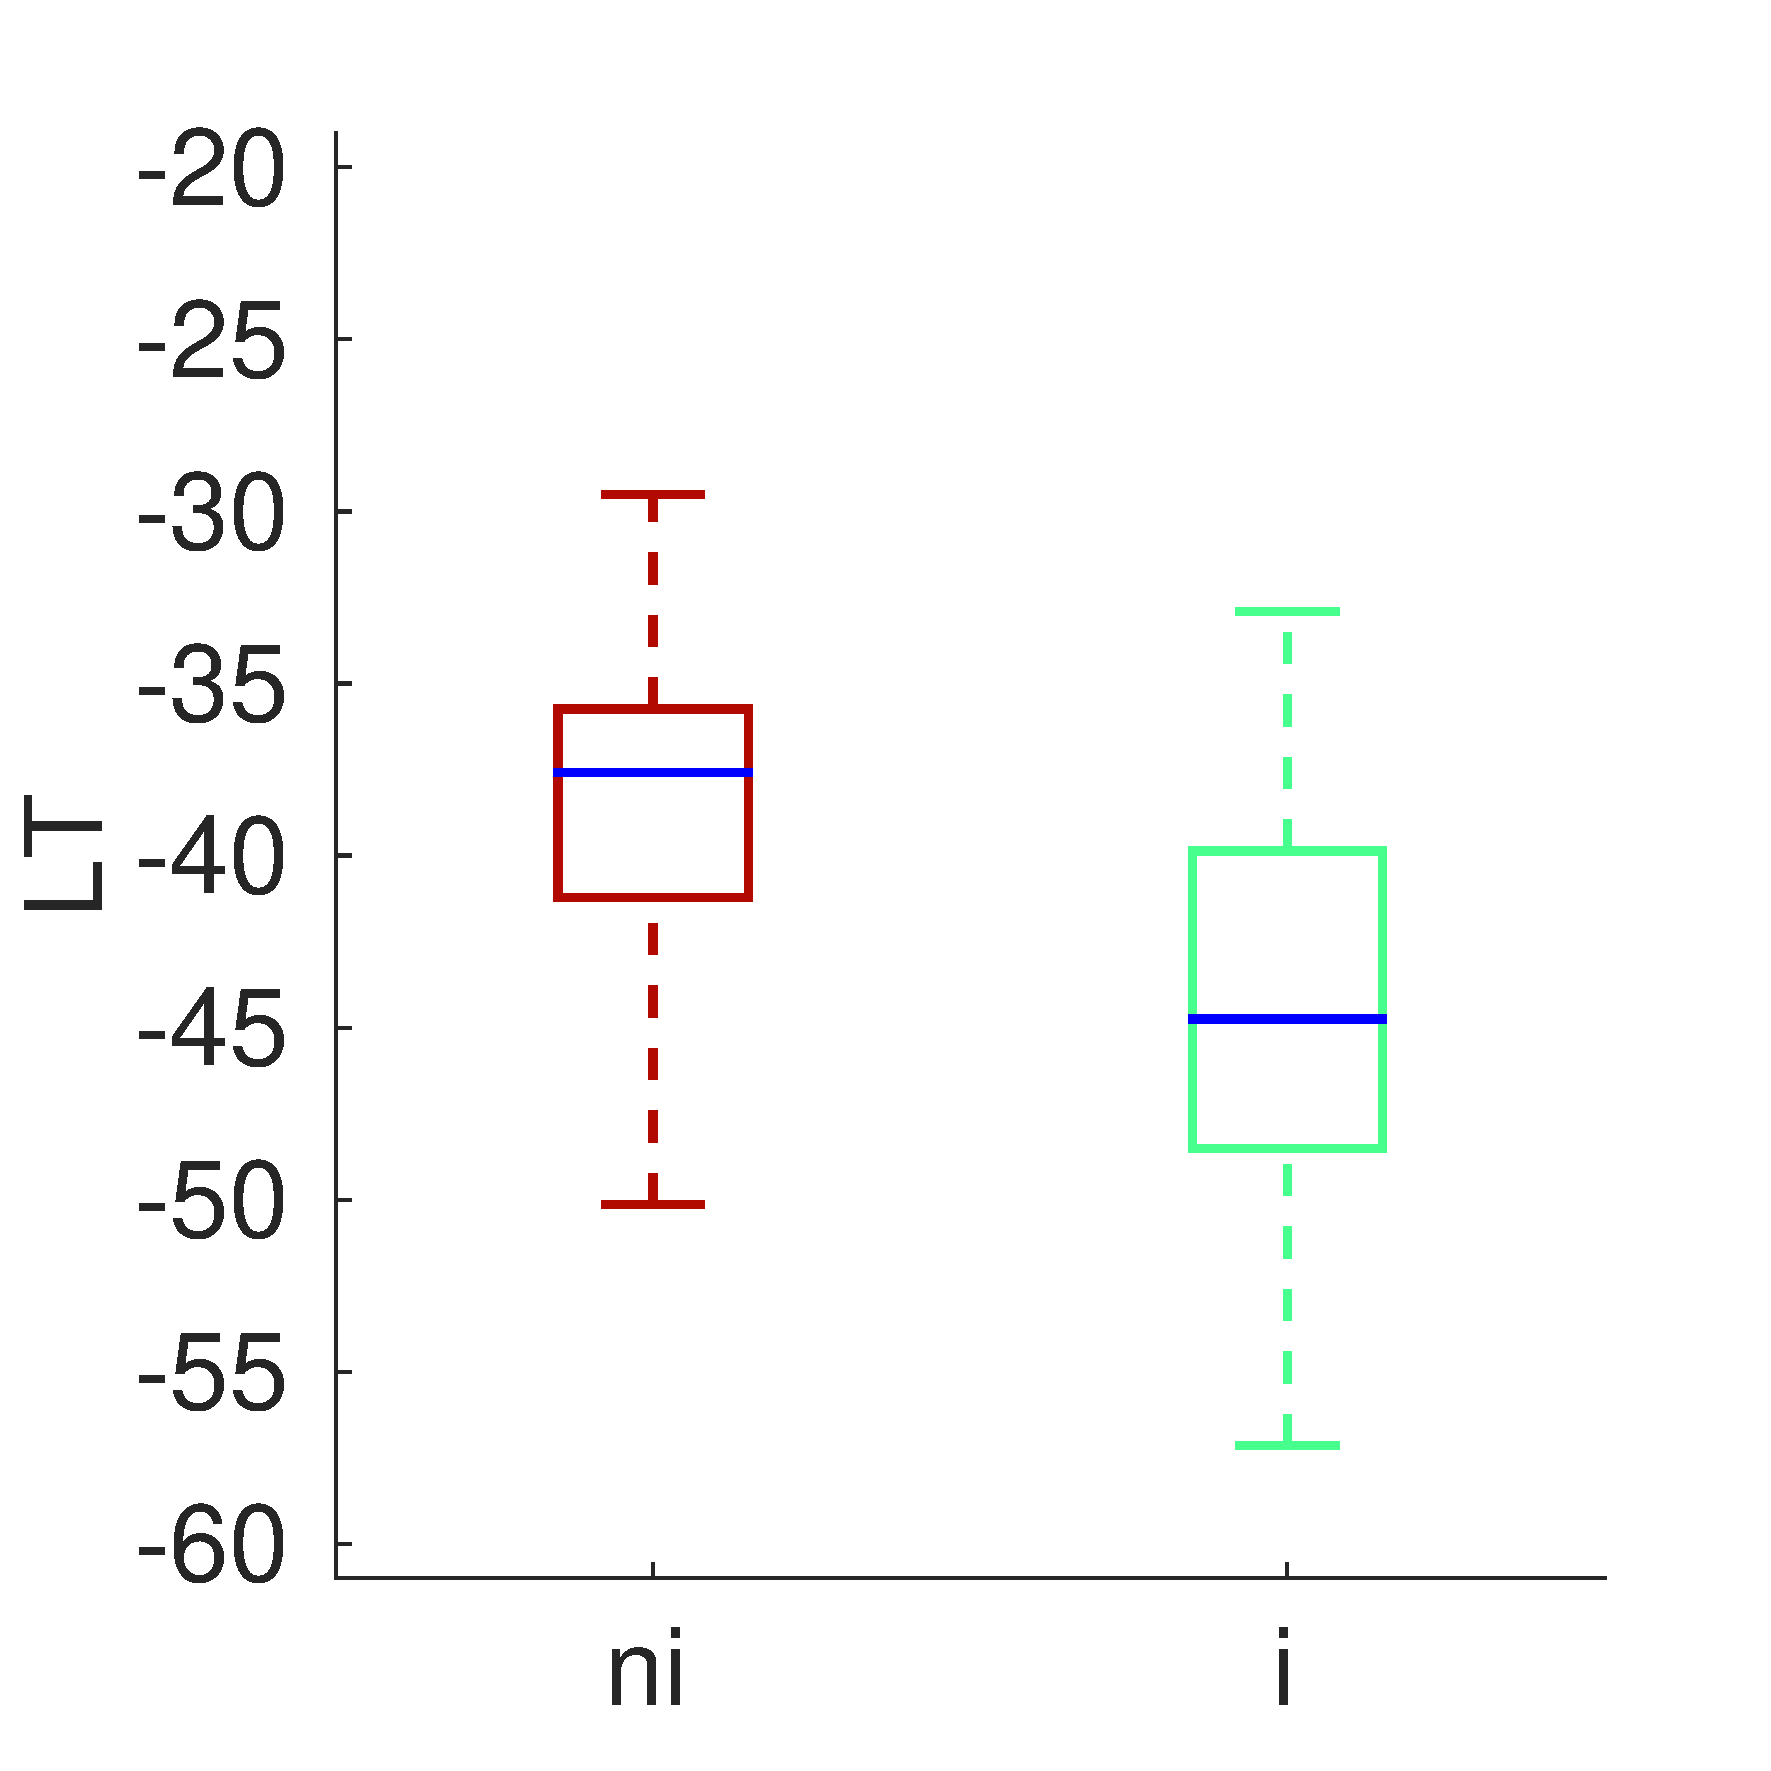
\includegraphics[width=.33\linewidth]{gfxXpUrbanSoundscape/xp_soundlevel_5}\label{fig:soundlevelc}}\par
        \subfloat[]
        {\includegraphics[width=.33\linewidth]{gfxXpUrbanSoundscape/xp_soundlevel_2}\label{fig:soundleveld}}
        \subfloat[]
        {\includegraphics[width=.33\linewidth]{gfxXpUrbanSoundscape/xp_soundlevel_4}\label{fig:soundlevele}}
        \subfloat[]
        {\includegraphics[width=.33\linewidth]{gfxXpUrbanSoundscape/xp_soundlevel_6}\label{fig:soundlevelf}}
       \caption[TODO]{TODO}\label{fig:soundlevel}
\end{figure}

\begin{figure}[t]
        \myfloatalign
        \subfloat[]
        {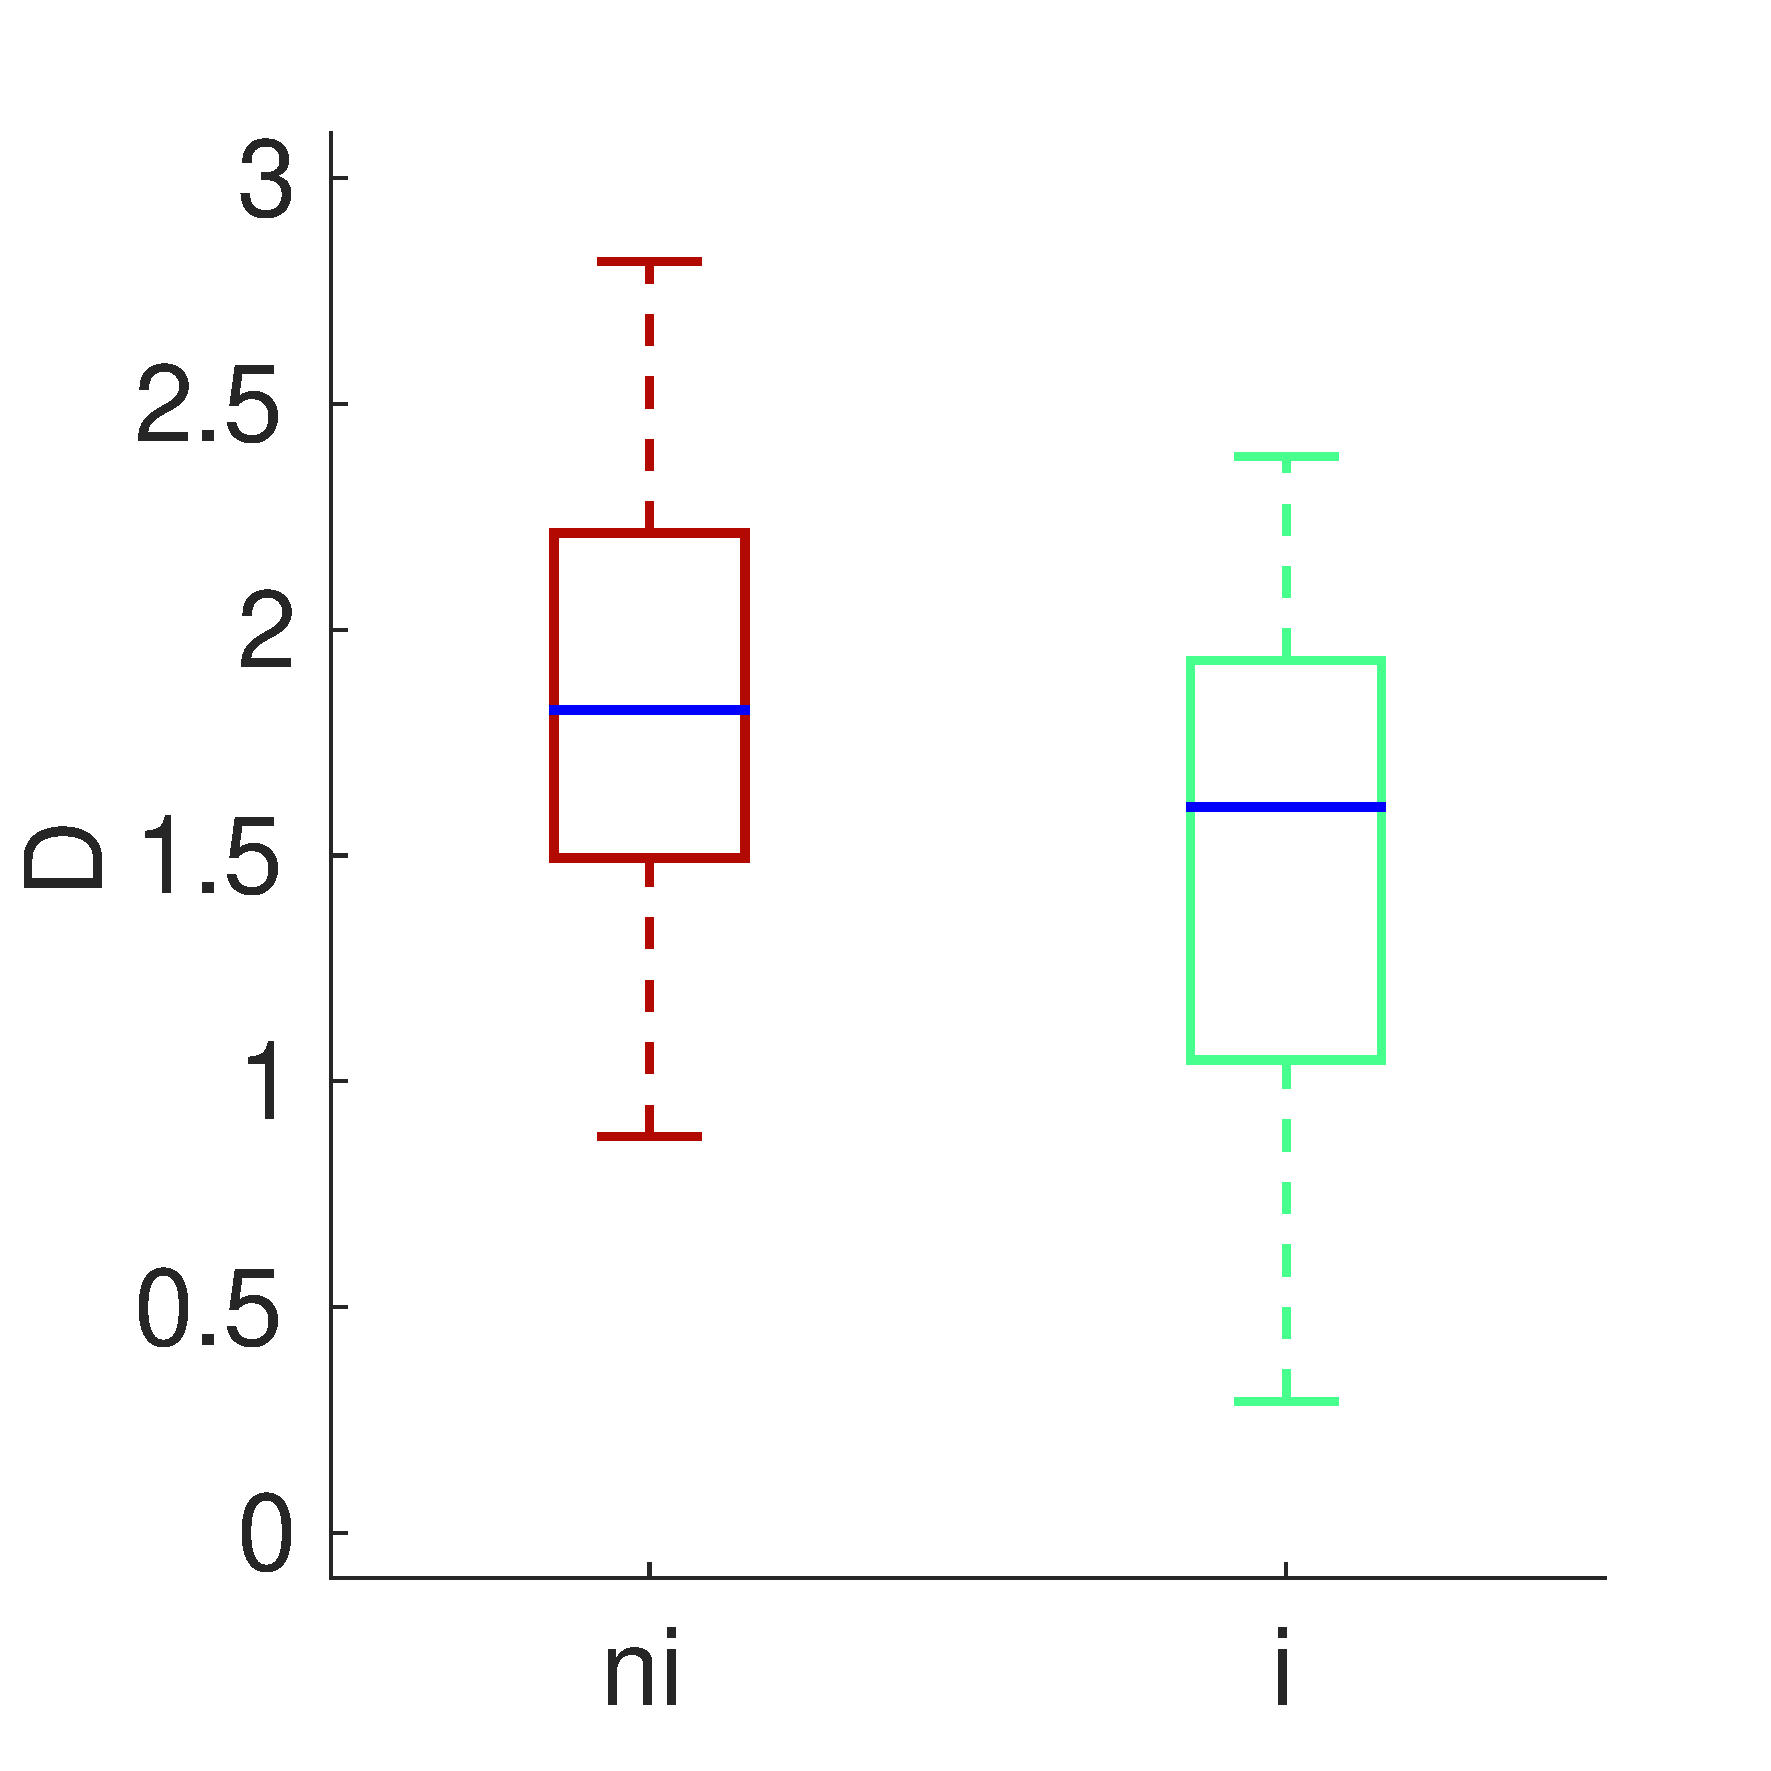
\includegraphics[width=.33\linewidth]{gfxXpUrbanSoundscape/xp_density_1}\label{fig:densitya}}
        \subfloat[]
        {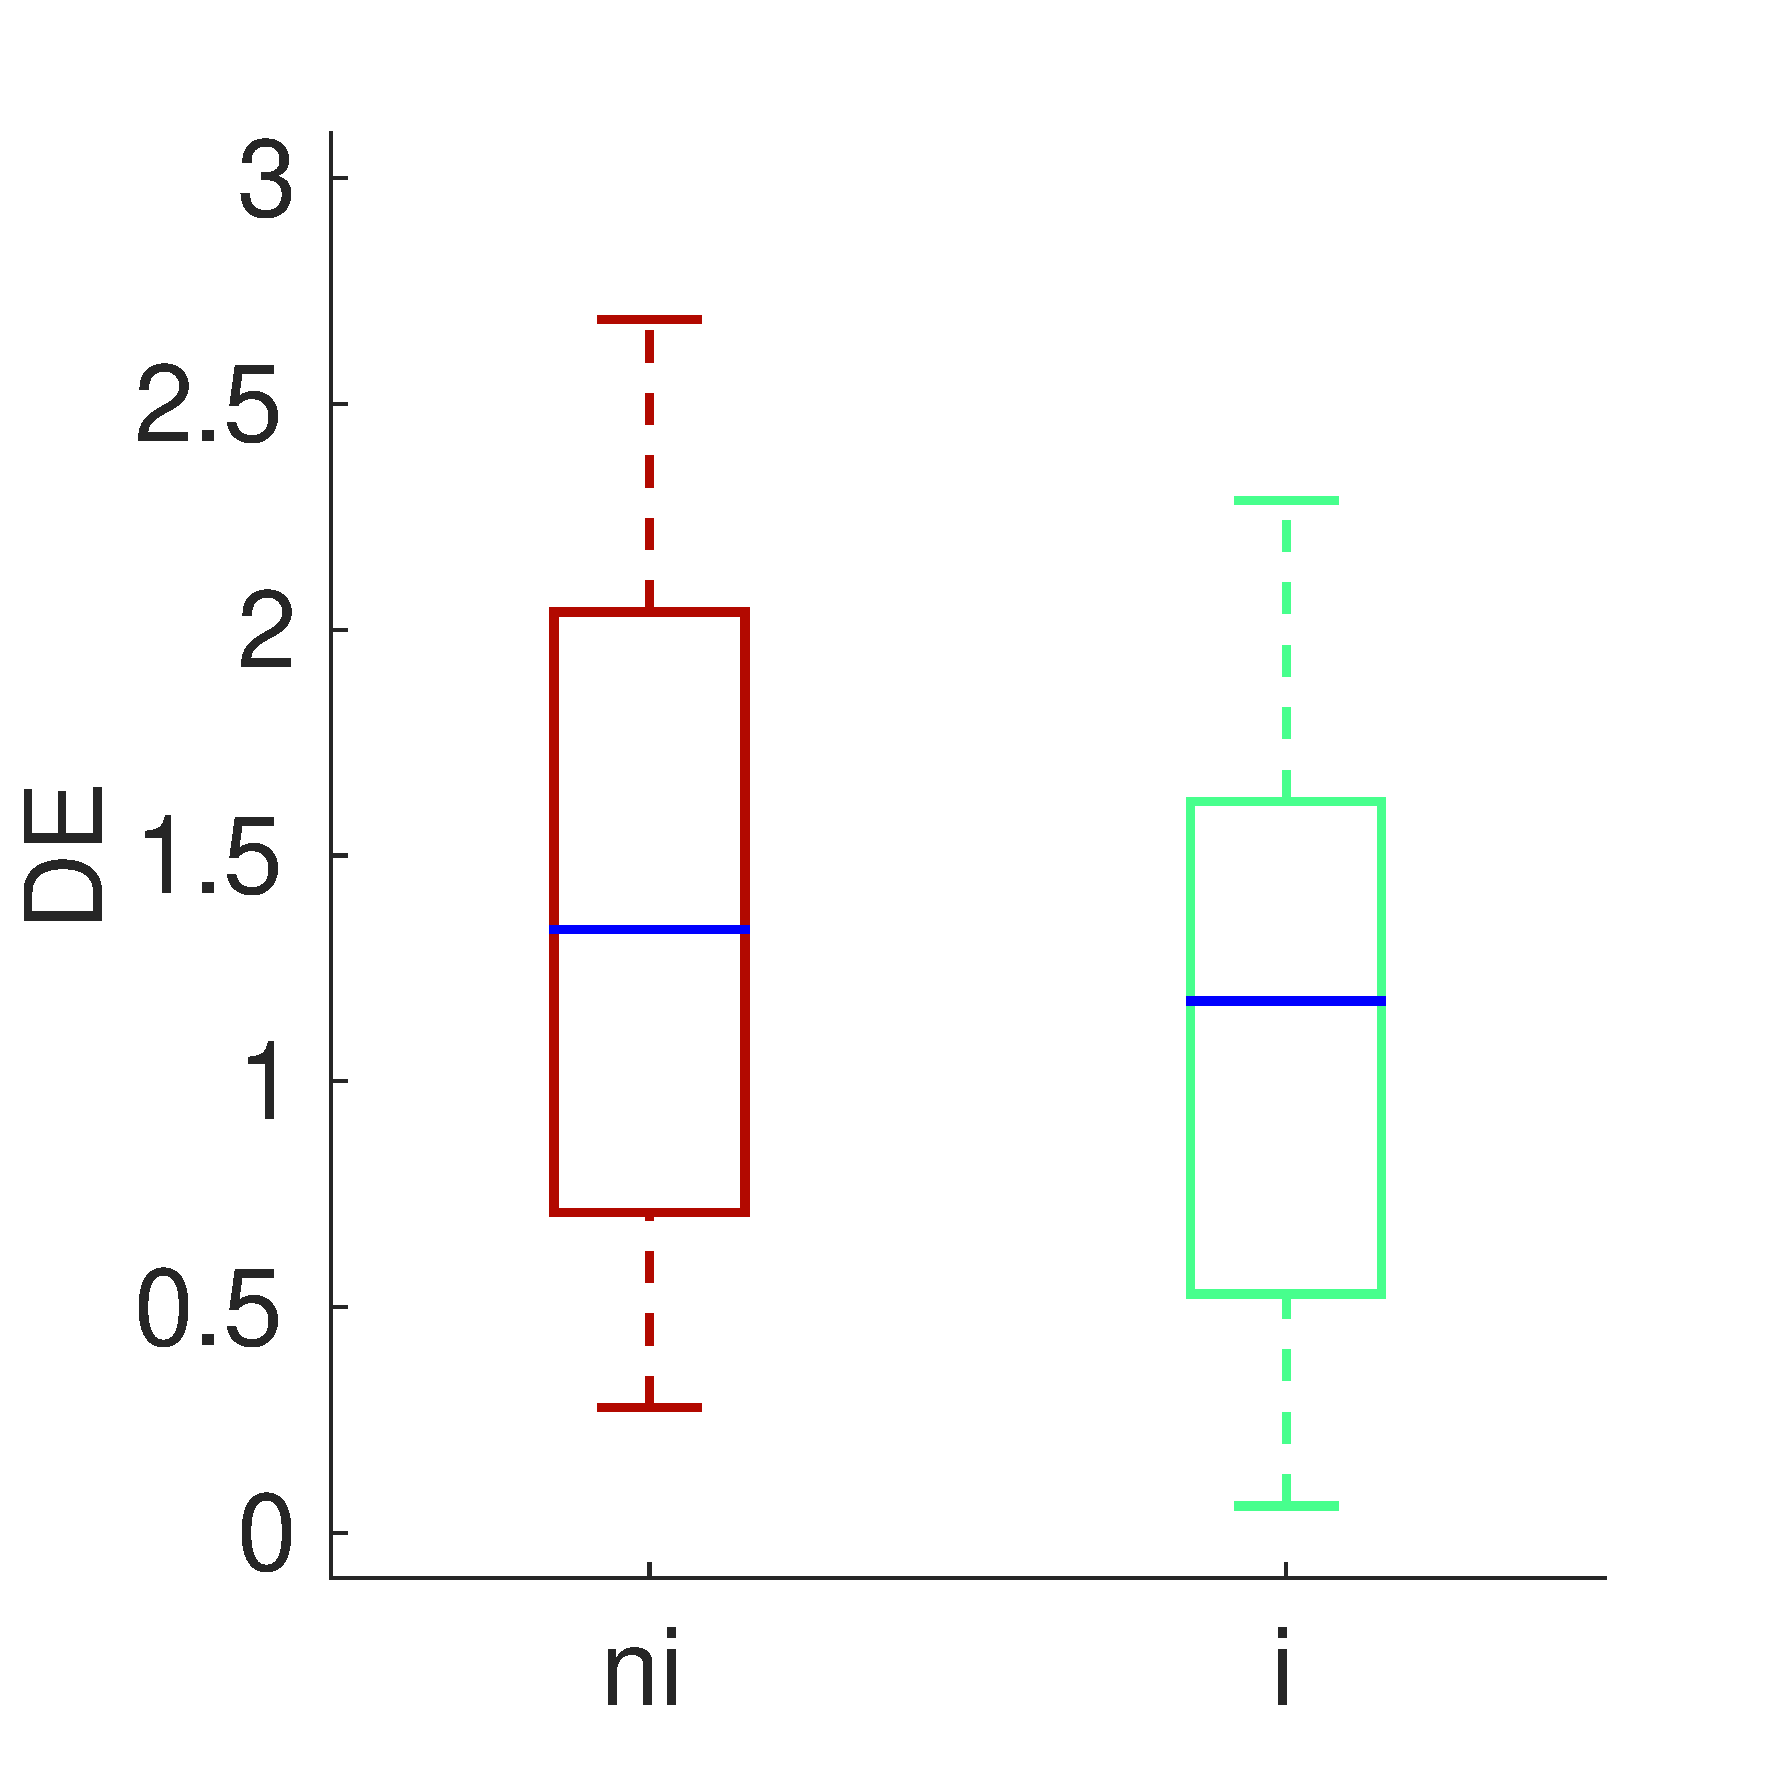
\includegraphics[width=.33\linewidth]{gfxXpUrbanSoundscape/xp_density_3}\label{fig:densityb}}\par
        \subfloat[]
        {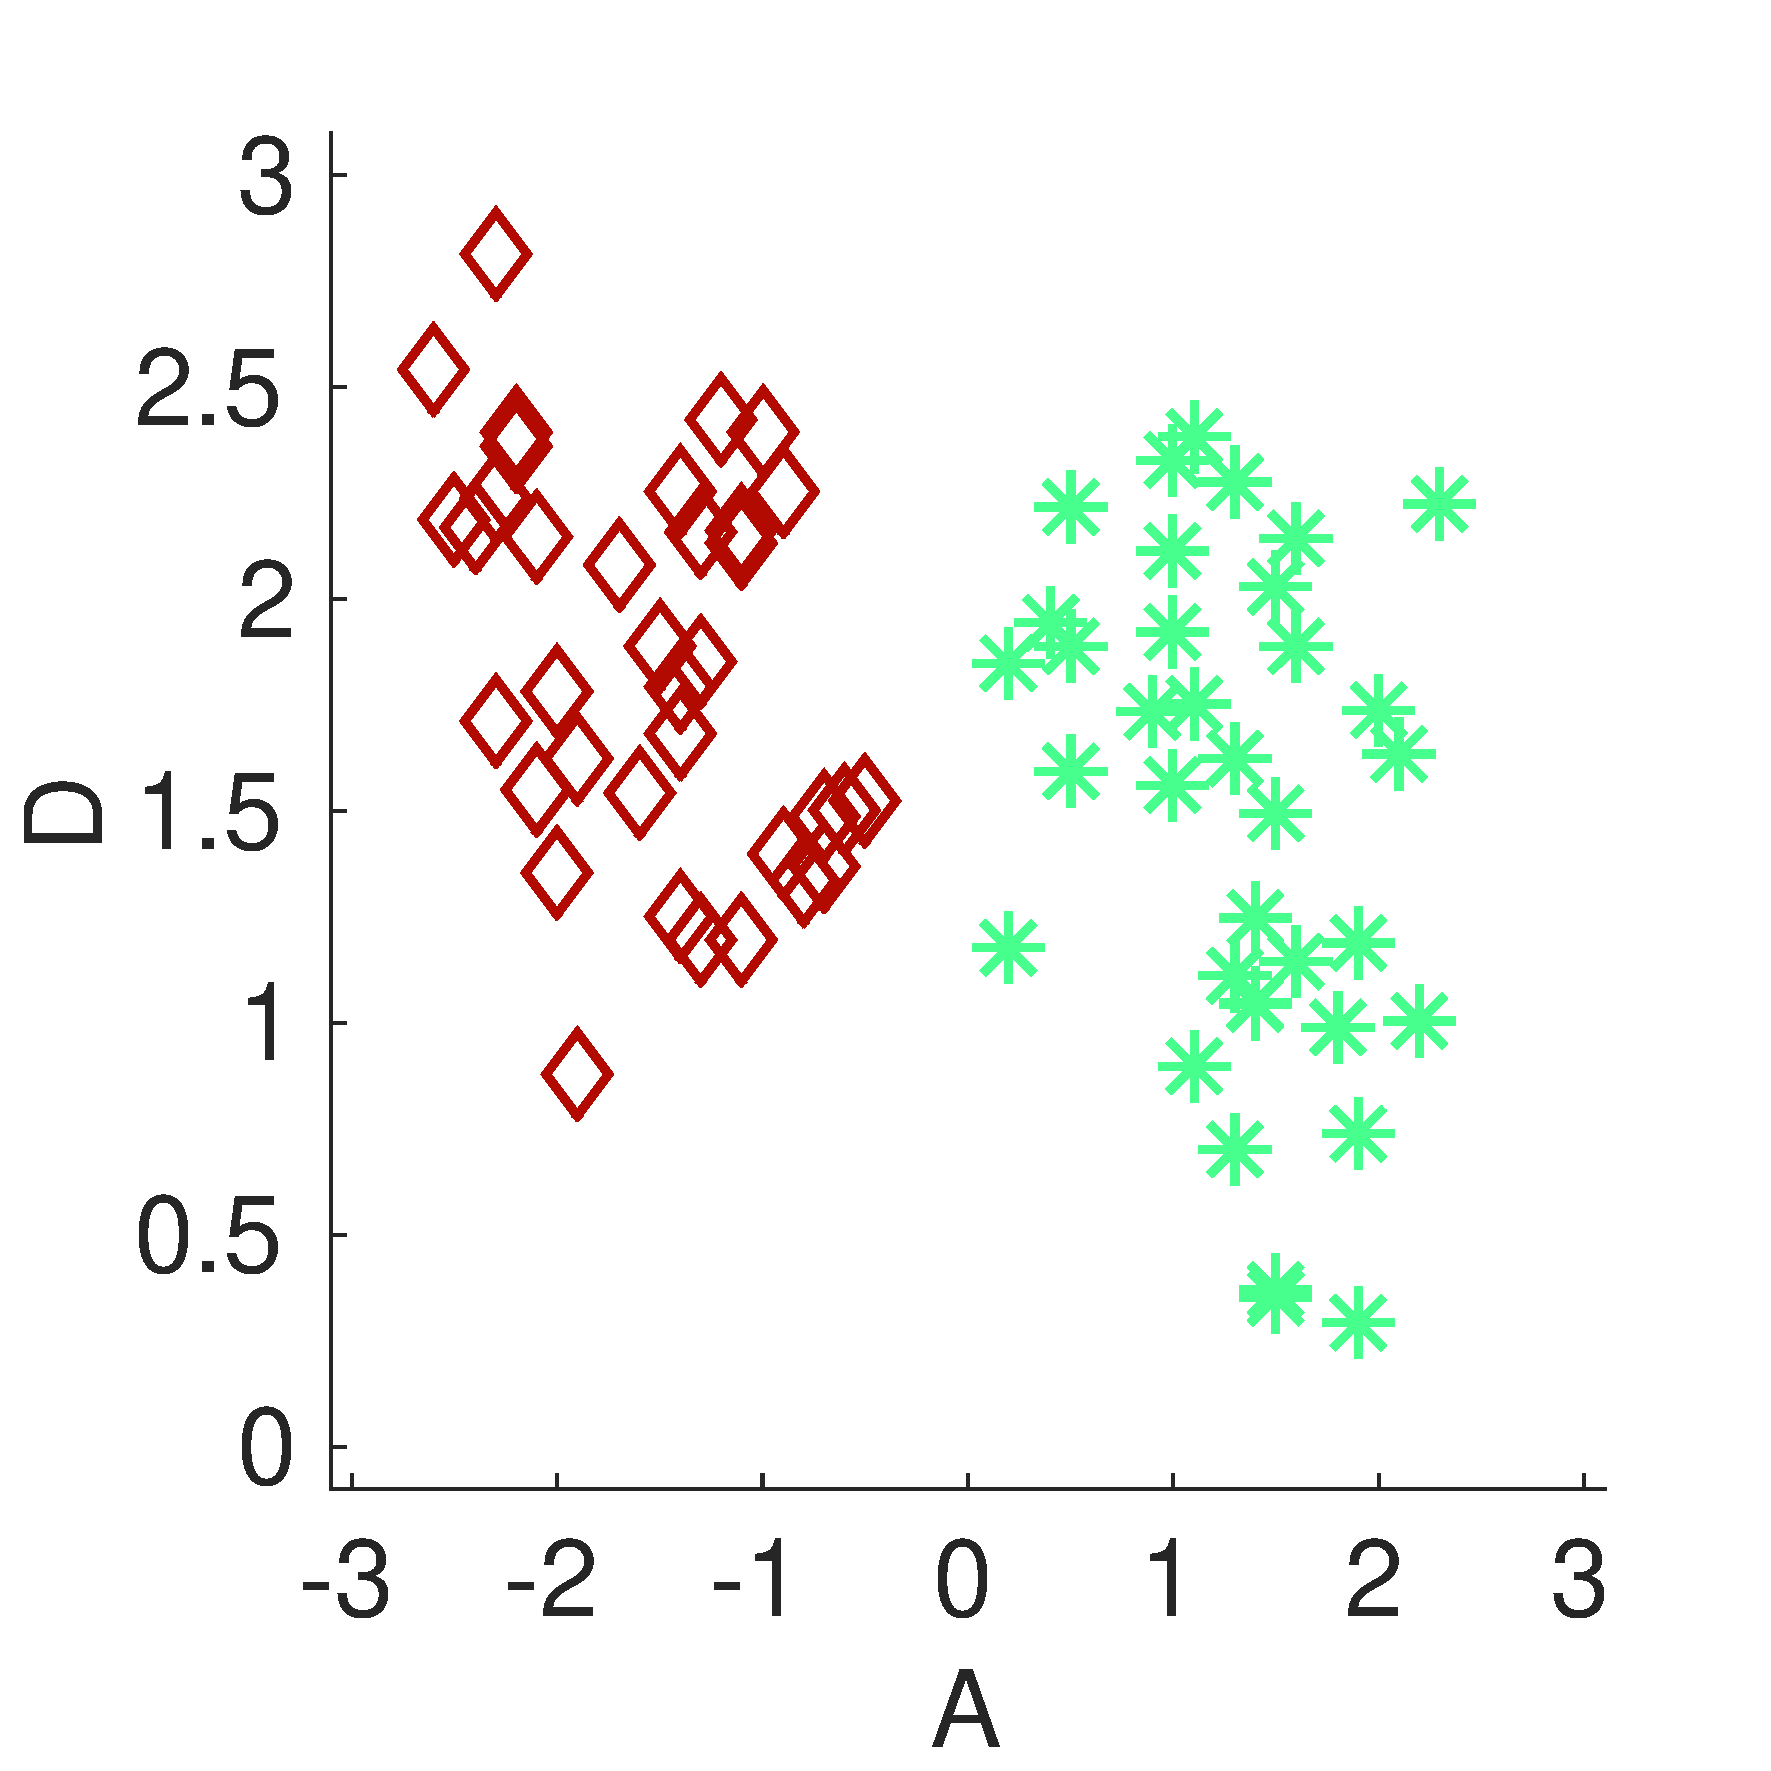
\includegraphics[width=.33\linewidth]{gfxXpUrbanSoundscape/xp_density_2}\label{fig:densityc}}
        \subfloat[]
        {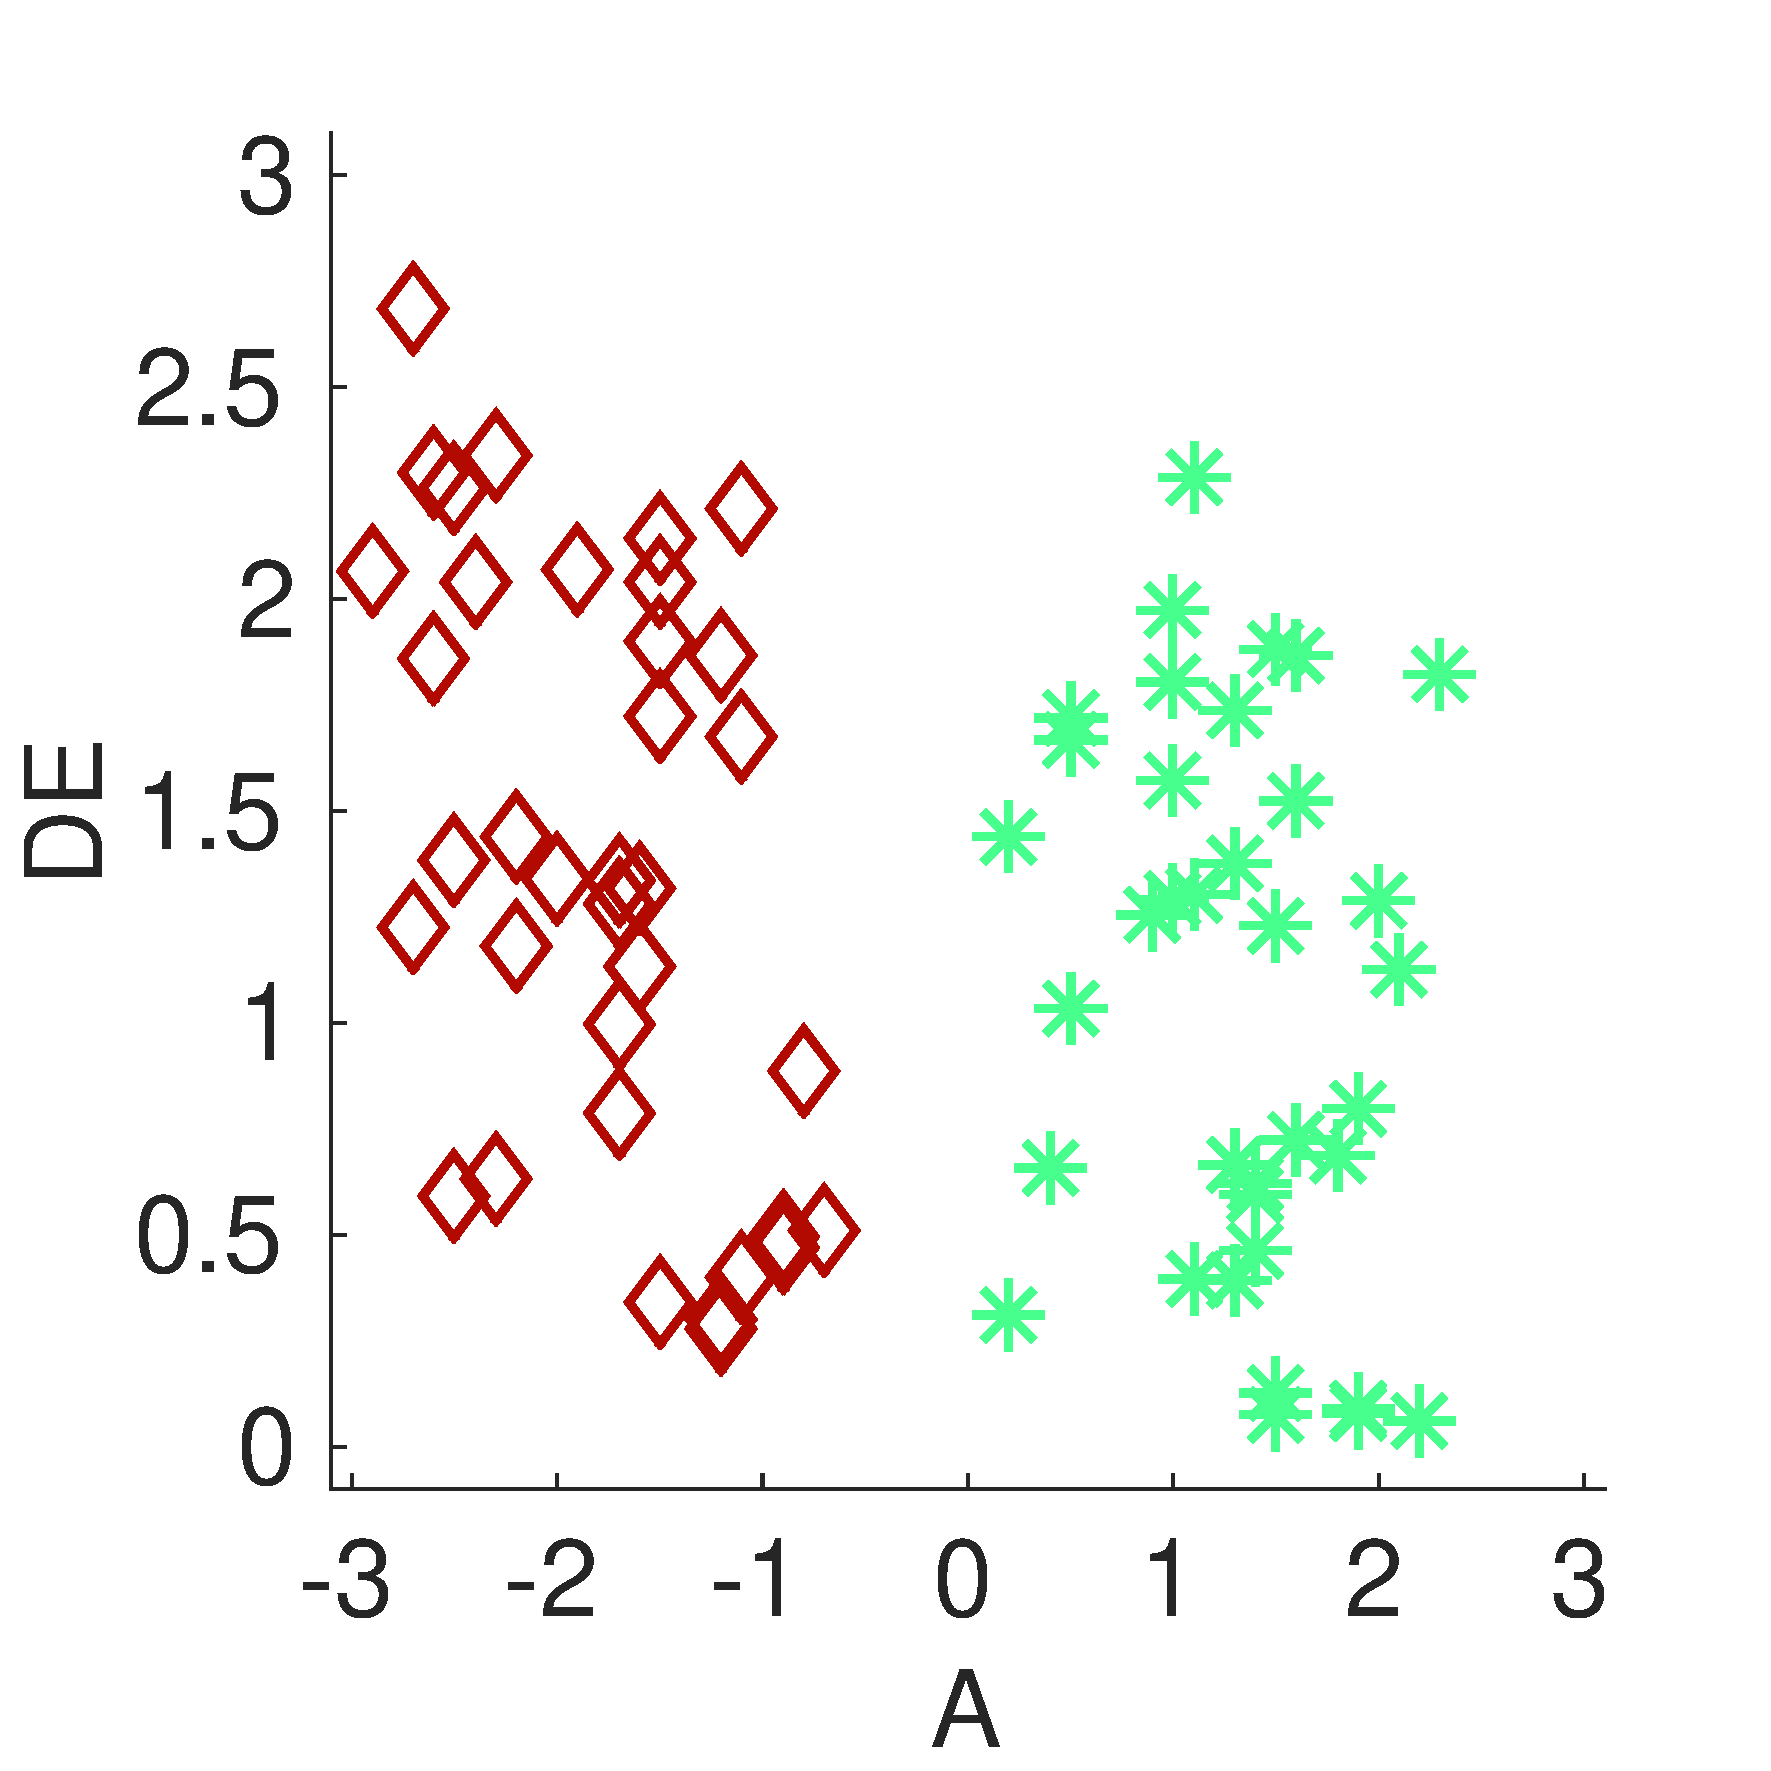
\includegraphics[width=.33\linewidth]{gfxXpUrbanSoundscape/xp_density_4}\label{fig:densityd}}
       \caption[TODO]{TODO}\label{fig:density}
\end{figure}

\begin{figure}[t]
        \myfloatalign
        \includegraphics[width=.8\linewidth]{gfxXpUrbanSoundscape/xp1_div_1}
       \caption[TODO]{TODO}\label{fig:diversity}
\end{figure}

\subsection{Influence des descripteurs structurels sur l'agrément perçu}
\label{sec:ch5_corrDesStruct}

Nous analysons, dans cette section, les relations fines qui peuvent exister entre les descripteurs structurels, d'une part, et l'agrément perçu, d'autre part. Contrairement à la section précédente, où la qualité affective des scènes est représentée de manière binaire (i \vs~ni), nous considérons, ici, l'agrément moyen $\mathcal{A}_{scene}$ comme descripteur perceptif. Il s'agit d'étudier l'existence de potentielles corrélations entre les descripteurs structurels et $\mathcal{A}_{scene}$. Les coefficients de corrélations linéaires calculés entre $\mathcal{A}_{scene}$ \vs~$L$, $L(E)$, $L(T)$, $D$, $D(E)$ et $DIV(E)$ sont présentés dans le tableau~\ref{tab:corrStructA}. Les relations entre $\mathcal{A}_{scene}$ et les descripteurs structurels sont illustrées par les figures~\ref{fig:soundleveld},~\ref{fig:soundlevele} et ~\ref{fig:soundlevelf}, pour les niveaux sonores, et les figures~\ref{fig:densityc} et~\ref{fig:densityd}, pour les densités. 

Concernant $L$, on observe une forte corrélation négative ($r=-0.77$, $p<0.01$) avec $\mathcal{A}_{scene}$, indiquant que plus le niveau sonore est élevé, plus la scène est désagréable. Cependant, la figure~\ref{fig:soundleveld} suggère que cette relation ne s'opère pas de la même manière pour les i- et ni-scènes. En effet, la corrélation entre $L$ et $\mathcal{A}_{scene}$, pour les ni-scènes, reste élevée ($r=-0.78$, $p<0.01$), mais est inexistante pour les i-scènes. 

Cette corrélation élevée, considérant l'ensemble des scènes, résulte du fait que les i-scènes ont tendance à être moins fortes que les ni-scènes, donnant ainsi l'illusion de prolonger la corrélation négative observée pour les ni-scènes.  

Nous en concluons que $L$:

\begin{itemize}
\item permet bien de faire la distinction entre les i- et ni-scènes,
\item permet de finement caractériser l'agrément perçu des ni-scènes,
\item n'est pas un indicateur pertinent de l'agrément perçu pour des environnements a priori agréables.
\end{itemize}

Les mêmes observations sont faites concernant $L(E)$ (\cf~\ref{fig:soundlevele}). Pour $L(T)$ (\cf~\ref{fig:soundlevelf}), bien que, à considérer l'ensemble des scènes, on observe une corrélation modérée, cela n'est pas vérifié quand on regarde séparément les i-scènes ($r=-0.33$, $p=0.05$) et les ni-scènes ($r=-0.00$, $p=0.99$). Là encore on peut penser que la corrélation négative observée pour l'ensemble des scènes est un artefact, résultant du fait que le niveau des textures des i-scènes a tendance à être plus bas que celui des ni-scènes. Ainsi, si les événements sonores conservent une certaine capacité de prédiction de l'agrément pour les ni-scènes, le niveau des textures n'apporte, lui, que peu d'informations, quel que soit l'environnement.

Considérant l'ensemble des scènes, nous observons une corrélation négative faible pour $D$ ($r=-0.44$, $p<0.01$) et $D(E)$ ($r=-0.34$, $p<0.01$). Une relation semblable est observée pour les ni-scènes ($D$: $r=-0.38$, $p<0.05$; $D(E)$: $r=-0.46$, $p<0.01$), mais aucune corrélation n'est observée pour les i-scènes. La densité de sources sonores semble donc avoir un faible impact sur l'agrément perçu, si l'on considère les ni-scènes, mais, comme pour les niveaux, cette densité ne semble pas avoir d'impact pour les i-scènes.

En ce qui concerne la diversité des classes d'événements, une corrélation négative faible est observée pour les niveaux d'abstraction 1, 2 et 3, en tenant compte de l'ensemble des scènes. Si l'on considère les i- et ni-scènes séparément, aucune corrélation significative n'est trouvée. Les conclusions sont similaires à celles faites pour $L(T)$: la diversité permet uniquement de faire la distinction entre les deux types d'environnements, mais ne permet pas de caractériser précisément l'agrément perçu.

En résumé, en présence d'un environnement désagréable, les niveaux sonores, en particulier ceux des événements, ainsi que, dans une moindre mesure, la densité de sources présentes, ont un impact négatif sur l'agrément. En présence d'un environnement agréable, aucun des descripteurs structurels considérés ici ne semble influer sur la perception de l'agrément. 

Ces premiers résultats pourraient montrer qu'il existe deux modes de perception, mobilisant chacun des descripteurs indépendants, modes qui s'activent en fonction de la nature de l'environnement (i ou ni).

Le fait qu'aucun des descripteurs globaux ne permettent de caractériser l'agrément des i-scènes peut nous amener à penser que toutes les sources sonores ne contribuent pas de manière égale à la perception de l'agrément, mais, que seules les caractéristiques de certaines d'entre elles ont une réelle influence. Afin d'approfondir ce point, nous analysons, dans la section suivante, les scènes d'un point de vue sémantique, \ie~en nous intéressant à la nature des sources qui les composent. \\


\begin{table}[t]
\centering
\begin{tabular}{l c c c} 
            & ensemble                     & i-scènes                   & ni-scènes    \\
\hline
$L$            & \textbf{-0.77} ($p<0.01$)    & -0.32 ($p=0.06$)           & \textbf{-0.78} ($p<0.01$)\\
$L(E)$         & \textbf{-0.75} ($p<0.01$)    & -0.20 ($p=0.24$)           & \textbf{-0.75} ($p<0.01$)\\
$L(T)$         & \textbf{-0.53} ($p<0.01$)    & -0.33 ($p=0.05$)           &  -0.00 ($p=0.99$) \\
$D$            & \textbf{-0.43} ($p<0.01$)    & -0.31 ($p=0.07$)           & \textbf{-0.38} ($p<0.05$)\\
$D(E)$         & \textbf{-0.34} ($p<0.01$)    & -0.22 ($p=0.21$)           & \textbf{-0.46} ($p<0.01$)\\
$DIV(E)$ 0     &          -0.07 ($p=0.52$)    & -0.25 ($p=0.15$)           & -0.23 ($p=0.23$)\\
$DIV(E)$ 1     & \textbf{-0.47} ($p<0.01$)    & -0.25 ($p=0.14$)           & -0.26 ($p=0.13$)\\
$DIV(E)$ 2     & \textbf{-0.41} ($p<0.01$)    & -0.21 ($p=0.22$)           & -0.25 ($p=0.14$)\\
$DIV(E)$ 3     & \textbf{-0.37} ($p<0.01$)    & -0.18 ($p=0.30$)           & -0.18 ($p=0.16$)\\
\hline
\end{tabular}
\vspace{0.5mm}
\caption{Coefficients de corrélation linéaire calculés entre l'agrément perçu moyen $\mathcal{A}_{scene}$ \vs~TODO}
\label{tab:corrStructA}
\end{table}

\subsection{Étude comparative entre les descripteurs sémantiques}

\subsubsection{Analyse qualitative}
\label{sec:ch5_anaQualiSem}

Nous analysons la composition des scènes en comptant le nombre de sujets ayant utilisé une classe de sons pour simuler un type d'environnements. Les résultats sont présentés à la figure~\ref{fig:soundsourcea} pour les événements, et à la figure~\ref{fig:soundsourceb} pour les textures. Par souci d'espace, nous choisissons un niveau d'abstraction intermédiaire entre le niveau 0 et 1, noté $0+$, pour représenter les classes (\cf~Figure~\ref{fig:taxonomie}).

Nous observons une différence notable dans le choix des classes entre les i- et ni-scènes. La répartition des classes est très proche de celle obtenue dans une étude similaire sur les environnements sonores urbains idéaux \citep{guastavino2006ideal}, \ie~les classes suggérant la présence humaine et la nature sont très présentes dans les i-scènes, a contrario, les classes désignant des sons mécaniques et/ou de travaux sont principalement utilisées pour les ni-scènes.

Ces résultats confirment un fait déjà observé: la nature sémantique des sources sonores joue un rôle prédominant dans l'appréciation de l'environnement \citep{raimbault2005urban,dubois2006cognitive}.

Nous notons quelques différences avec \citep{guastavino2006ideal}: les résultats obtenus par Guastavino montrent que les sons de \emph{transports publics} sont caractéristiques des environnements sonores urbains idéaux. Les auteurs attribuent cela au fait que la perception de l'agrément est, entre autre, soumise à un contexte socio-culturel. Dans notre représentation du monde, les sons de transports publics sont positivement connotés, et ont ainsi tendance à être mieux acceptés que les sons de véhicules privés.

Dans une certaine mesure, nos résultats contredisent ce fait. La figure~\ref{fig:soundsourcea} montre, en effet, que les classes d'événements de \emph{transports publics} (\emph{bus} et \emph{train}, \cf~Figure~\ref{fig:soundsourcec}) ont été utilisées par les sujets, pour des i-scènes, dans $28\%$ des cas, et pour des ni-scènes, dans $42\%$ des cas. Les résultats ne remettent pas en question le fait que les sons de \emph{transports publics} soient bien acceptés: $25\%$ des sujets ont utilisé la classe \emph{bus} pour les i-scènes, un chiffre comparable à celui de la classe \emph{Vélo}, et bien supérieur à celui de toute autre classe de véhicules privés. Cependant les classes \emph{transports publics} sont également bien présentes dans les ni-scènes, plus que les classes \emph{voiture} ou \emph{camion} par exemple. La classe \emph{transports publics} ne peut donc pas être considérée comme typique d'un environnement sonore urbain idéal.

Cette différence peut s'expliquer par la nature des deux protocoles expérimentaux utilisés. Comme nous l'avons fait, Guastavino demande à ses sujets de décrire un environnement en se basant sur leurs mémoires. Mais, contrairement à nous, ils ne disposent pas de supports sonores. Le fait que nos sujets soient confrontés à la réalité acoustique des sons, pour recréer leurs environnements, peut avoir pour effet de diminuer l'impact du contexte socio-culturel. D'autres études utilisant des sons comme stimuli montrent que la classe \emph{bus} peut avoir un effet négatif sur l'appréciation de l'environnement \citep{lavandier2006contribution}.

\begin{figure}[t]
        \myfloatalign
        \subfloat[]
        {\includegraphics[width=.8\linewidth]{gfxXpUrbanSoundscape/xp1_class_1}\label{fig:soundsourcea}} \par
        \subfloat[]
        {\includegraphics[width=.4\linewidth]{gfxXpUrbanSoundscape/xp1_class_2}\label{fig:soundsourceb}} 
        \subfloat[]
        {\includegraphics[width=.4\linewidth]{gfxXpUrbanSoundscape/xp1_class_3}\label{fig:soundsourcec}} 
       \caption[TODO]{TODO}\label{fig:soundsource}
\end{figure}

\subsubsection{Marqueurs sonores}

Nous avons mis en évidence que, qualitativement, la composition des sources sonores des scènes diffère selon les types d'environnements (i ou ni). Nous essayons de voir maintenant si, parmi ces classes, certaines sont typiques d'un environnement en particulier. Pour ce faire, nous utilisons le V-test (\cf~Section~\ref{sec:ch5_methodoEtStat1}), en considérant séparément chaque niveau d'abstraction. Les résultats sont présentés dans le tableau~\ref{tab:markers}.

Concernant les événements sonores, 9 marqueurs sont identifiés sur l'ensemble des niveaux d'abstraction. Comme la figure~\ref{fig:soundsource} le laissait présager, les classes relatives à l'activité humaine (\emph{pas homme béton}, \emph{sonnette vélo}), et à la nature (\emph{animaux, oiseaux}, \emph{chants d'oiseaux}) sont des marqueurs de i-scènes. Nous notons également la présence de la classe \emph{cloche} dans les marqueurs d'un environnement idéal. Ce fait est possiblement dû au \emph{background} socio-culturel des sujets, dans leur grande majorité, des citoyens européens. En effet, selon Schafer, un son reconnu par un individu comme faisant partie intégrante de son environnement est bien accepté. Les marqueurs de ni-scènes sont des classes faisant référence à des sons de travaux (\emph{travaux}), ou suggérant un trafic dense (\emph{klaxon}, \emph{sirène}).

Concernant les textures sonores, 5 marqueurs sont identifiés. Pour les i-scènes, il s'agit de classes faisant référence à des ambiances amorphes, calmes, (\emph{cour-intérieur/parc} et \emph{parc}). Pour les ni-scènes, il s'agit, comme pour les événements, de classes faisant référence à des bruits de travaux (\emph{travaux} et \emph{véhicule de travaux}), ainsi que d'une classe faisant référence au trafic (\emph{carrefour}).


\gl{Bien que l'ensemble des marqueurs identifiés soient intuitifs, aucune des classes d'événements faisant directement référence aux bruits de véhicules motorisés n'est un marqueur, exception faite de la classe de texture \emph{carrefour}}. Pour représenter un trafic désagréable, les sujets ont porté leurs choix sur les classes \emph{klaxon} et \emph{sirène}. On peut supposer que les sons isolés de véhicules sont compris comme faisant partie intégrante de l'environnement urbain, et ne sont donc pas particulièrement associés à un environnement désagréable. \\ 

\gl{TODO: ici analyse des caractéristiques des classes trafics} \\
\gl{TODO: ici reprendre les conclusions de \citep{lavandier2006contribution} et \citep{ricciardi2015sound}}

\begin{table}[t]
 \setlength{\tabcolsep}{0.2pt}
 \centering
  {\renewcommand{\arraystretch}{0.9}
\begin{tabular}{c c c c} 
Niveau        & \multicolumn{2}{c}{Marqueurs sonores événements} \\
d'abstraction & i-scènes & ni-scènes \\
\hline
0  &                               &  construction work (3.78)  \\
\hline
  & church bell  (4.5)             & horn  (3.9) \\
1 & bell bike    (4.3)             & siren (3.9)\\
  & animal       (4.2)             &       \\
   \hline
  & birds        (4.8)             & horn  (4.0)\\
2 & church bell  (4.4)             & siren (4.0)\\
  & bell bike    (4.2)             &       \\
   \hline
  & birds singing (4.8)            & horn  (4.1)\\
  & church bell   (4.3)            & siren (4.0)\\
3 & bell bike     (4.2)            &       \\
  & male footsteps                 &  \\
  &   concrete (3.6)               &  \\
  &                                & \\ 
  & \multicolumn{2}{c}{Marqueurs sonores textures}      \\
  & i-scènes & ni-scènes \\
\hline
0 &     courtyard/park (4.1)       &  construction work (3.9)  \\
\hline
1 &     park (3.65)                &  crossroads (3.6)  \\
  &                                &  vehicle work (3.3)  \\
\hline
2 &     park (3.64)                &  crossroads (3.56)  \\
\hline
\end{tabular}
}
\vspace{0.5mm}
\caption[Classes d'événements identifiées comme étant des marqueurs sonores]{Classes d'événements identifiées comme étant des marqueurs sonores. Dans chaque cellule, les marqueurs sont ordonnés par ordre décroissant de valeur $V$.}
\label{tab:markers}
\end{table}

\subsection{Étude des espaces de représentation induits par les descripteurs sémantiques}

Dans cette partie, nous évaluons la capacité d'une représentation sémantique à séparer les deux types d'environnements. Pour ce faire, nous calculons une précision au rang 5 ($p@5$) sur l'espace induit par les descripteurs sémantiques $S$, et ce pour chaque niveau d'abstraction (\cf~Section~\ref{sec:ch5_methodoEtStat1}). Les vecteurs $S$ sont construits en utilisant toutes les classes ($ET$), les classes d'événements ($E$), les classes de textures ($T$), les classes d'événements ne considérant que les marqueurs sonores ($E_m$), les classes d'événements ne considérant pas les marqueurs sonores $E_{w/o,m}$. Les résultats sont affichés sur la figure~\ref{fig:pa5}.

En ce qui concerne $ET$, la $p@5$ est de $76\%$ pour le niveau d'abstraction 0, et reste supérieure à $86\%$ à partir du niveau d'abstraction 1. Ces résultats confirment qu'il est possible de clairement distinguer les deux types d'environnements en se basant seulement sur la présence ou l'absence des classes de sons. Nous notons également que, plus le niveau d'abstraction est élevé, plus la capacité de séparer les environnements est importante. En d'autres termes, plus nous sommes précis dans notre description de la composition des scènes, plus nous sommes à même d'établir une distinction claire entre les i- et ni-scènes.

En considérant séparément $E$ et $T$, il apparaît que 1) la $p@5$ obtenue avec $E$ est similaire à celle obtenue avec $ET$, et 2) que la $p@5$ obtenue avec $T$ est systématiquement inférieure d'environ $10$ à $15\%$ à celle de $E$. Ces résultats indiquent que l'information sémantique permettant de séparer les deux environnements est principalement portée par les événements. Ces résultats font, par ailleurs, écho aux travaux de  \citep{maffiolo_caracterisation_1999}, qui montrent que nous analysons de manière descriptive (en identifiant les sources) les scènes événementielles, \ie~composées d'événements sonores (\cf~Section~\ref{sec:ch3_catsoundscape}).

Enfin, il apparaît que la $p@5$ obtenue avec $E_{m}$ est similaire, voire supérieure à celles de $E$ et $ET$, et ce bien qu'une information partielle soit utilisée dans ce cas pour décrire les scènes. La dimension des vecteurs de description $S$ pour $E_m$ est en effet inférieure à la dimension des vecteurs $S$ pour $E$, qui est elle même inférieure à celle obtenue dans le cas où toutes les classes sont utilisées ($ET$). De plus, dans le cas où les marqueurs ne sont pas pris en compte pour la description ($E_{w/o,m}$), les résultats chutent, passant même en dessous de ceux obtenus en ne considérant que les textures. Cela confirme que la majorité de l'information sémantique permettant de faire la distinction entre i-scènes et ni-scènes est incluse dans les marqueurs.

En résumé, nous déduisons de cette analyse les points suivants:

\begin{enumerate}
\item contrairement à ce que nous avions constaté avec les descripteurs structurels, une description sémantique de la composition des scènes, en terme de présence/absence de sources sonores, permet de bien distinguer les deux types d'environnements (i ou ni);
\item l'information sémantique est majoritairement portée par les classes d'événements sonores;
\item parmi les classes d'événements, seule une partie, \ie~les marqueurs sonores, sont nécessaires afin de faire la distinction entre les i- et ni-scènes.
\end{enumerate}

Maintenant que nous avons isolé les classes typiques des i- et ni-scènes, et vérifié que la distinction entre ces environnements dépendait de la présence de ces classes, il reste à voir si une description structurelle des scènes, basée uniquement sur ces marqueurs sonores, permet de caractériser l'agrément perçu, mieux qu'une description structurelle globale. \\

\gl{analyse marqueur texture ?}\\
\gl{HCA sur $S$, + ANOVA sur $\mathcal{A}_{scene}$}

\begin{figure}[t]
        \myfloatalign
        \includegraphics[width=.8\linewidth]{gfxXpUrbanSoundscape/pa5_1}
       \caption[TODO]{TODO}\label{fig:pa5}
\end{figure}

\subsection{L'influence spécifique des marqueurs sonores sur l'agrément perçu}

\begin{table}[t]
\centering
\begin{tabular}{l r r} 
                  &   i-scenes                  & ni-scenes \\
\hline
$L_m$              & 0.03  ($p=0.88$)           & \textbf{-0.75} ($p<0.01$) \\
$L(E)_m$           & 0.08  ($p=0.66$)           & \textbf{-0.71} ($p<0.01$) \\
$L(T)_m$           & -0.11 ($p=0.66$)           & -0.17 ($p=0.37$) \\
$L_b$              & \textbf{-0.52} ($p<0.01$)  & -0.32 ($p=0.06$) \\
$L(E)_b$           & \textbf{-0.51} ($p<0.01$)  & -0.30 ($p=0.07$) \\
$L(T)_b$           & -0.32 ($p=0.05$)           & \textbf{-0.73} ($p<0.01$) \\
$L_m-L_b$          & \textbf{0.67} ($p<0.01$)   & -0.31 ($p=0.07$) \\
$L(E)_m-L(E)_b$    & \textbf{0.66} ($p<0.01$)   & -0.28 ($p=0.10$) \\
$L(T)_m-L(T)_b$    & 0.16 ($p=0.54$)            & 0.21 ($p=0.28$) \\
$D_m$              & 0.03 ($p=0.85$)            & -0.31 ($p=0.07$) \\
$D(E)_m$           & 0.09 ($p=0.62$)            & \textbf{-0.44} ($p<0.01$) \\
\hline
\end{tabular}
\vspace{0.5mm}
\caption{Coefficients de corrélation linéaire calculés entre l'agrément perçu moyen $\mathcal{A}_{scene}$ \vs~TODO.}
\label{tab:corrMarkers}
\end{table}

Comme pour la  section~\ref{sec:ch5_corrDesStruct}, nous évaluons les corrélations entre $\mathcal{A}_{scene}$ et les descripteurs structurels. Pour cette section, les descripteurs structurels sont calculés en tenant compte des marqueurs sonores précédemment identifiés. Nous définissons $X_m$ le descripteur $X$ calculé en ne prenant en compte que les sons des marqueurs. A l'inverse, nous définissons $X_b$ ($b$: pour ``\,bruit\,'') le descripteur $X$ calculé en prenant en compte toutes les classes de sons excepté les marqueurs. Lorsque le descripteur caractérise une i-scène (idem pour une ni-scène), nous ne considérons, pour le calcul, que les marqueurs identifiés pour les i-scènes (ou pour les ni-scènes), que nous nommons i-marqueurs (ou ni-marqueurs). Les résultats sont affichés sur le tableau~\ref{tab:corrMarkers}.

Considérons dans un premier temps les densités (\cf~Figures~\ref{fig:densityMarker}). Les résultats pour $D_m$ et $D(E)_m$ sont similaires à ceux observés précédemment pour $D$ et $D(E)$, a l'exception de $D_m$  qui ne présente plus une corrélation significative pour les ni-scènes. Ces résultats tendent à confirmer que la densité est un indicateur d'agrément de faible importance, qu'on la considère globalement, ou en prenant en compte les contributions séparées de différentes sources. \\

\gl{TODO: Rajouter $D_b$} \\

Concernant les niveaux sonores (\cf~Figures~\ref{fig:soundlevelMarker}), là encore les mêmes tendances sont observées entre $L_m$, $L(E)_m$ et $L(T)_m$, d'une part, et $L$, $L(E)$ et $L(T)$, d'autre part. Que l'on considère uniquement les marqueurs, ou l'ensemble des classes, il s'avère que :

\begin{enumerate}
\item Il existe une différence significative entre les niveaux des i- et ni-scènes ($L_m$, $L(E)_m$ et $L(T)_m$: $p<0.01$) 
\item Le niveau sonore des scènes est majoritairement porté par les événements sonores.
\item Le niveau sonore des événements a une influence sur la perception de l'agrément pour les ni-scènes, mais pas pour les i-scènes.
\item Le niveau sonore des textures ne joue aucun rôle dans la perception de l'agrément
\end{enumerate}

En conclusion, le niveau des ni-marqueurs a une influence négative sur l'agrément pour les ni-scènes, en revanche le niveau des i-marqueurs n’impacte pas l'agrément perçu pour les i-scènes.

En considérant maintenant les classes non marqueurs  (\cf~Figures~\ref{fig:soundlevelNoise}), nous remarquons, sur les i-scènes, une corrélation négative modérée/faible pour $L_b$  ($r=-52$, $p<0.01$) et $L(E)_b$ ($r=-51$, $p<0.01$). C'est la première fois qu'un indicateur objectif nous permet de préciser l'agrément des environnements agréables. Ceci nous amène à conclure que le niveau des classes de sons n'étant pas typiques d'un environnement agréable a un impact négatif sur l'agrément. 

Par ailleurs, alors que $L(T)$ ne présentait pas de corrélation pour les ni-scènes, une corrélation négative forte est observée pour $L(T)_b$ ($r-0.73$, $p<0.01$). Ce fait indique que des classes de textures, utilisées pour simuler aussi bien les i-scènes que les ni-scènes, n'affectent pas l'agrément perçu de la même manière. Pour une même classe \emph{foule}, le niveau perçu dans un cadre idéal n'affectera pas la perception de l'agrément, alors que dans un cadre non-idéal, il impactera négativement le ressenti \gl{TODO: chiffre}.

Pour finir, nous considérons un dernier groupe de descripteurs, nommément $L_m-L_b$, $L(E)_m-L(E)_b$ et $L(T)_m-L(T)_b$ (\cf~Figures~\ref{fig:soundlevelMarkerDiff}). Ces descripteurs expriment la différence entre les niveaux des marqueurs, et ceux des autres classes de sons. Ils traduisent l'émergence des marqueurs par rapport à la mixture sonore.

Pour les i-scènes, une corrélation modéré et positive est observée pour $L_m-L_b$ ($r=0.67$, $p<0.01$) et $L(E)_m-L(E)_b$ ($r=0.66$, $p<0.01$). Pour les ni-scènes, aucune corrélation n'est observée. Dans le cas des i-scènes, ce n'est donc pas le niveau absolu des marqueurs qui importe, mais leur niveau relatif, par rapport aux autres sons qui composent la scène. On observe donc pour les environnements idéaux un double mécanisme perceptif: 

\begin{itemize}
\item plus le niveau absolu des sons n'étant pas des i-marqueurs est élevé, plus l'agrément est faible,
\item plus le niveau relatif des i-marqueurs, par rapport aux autres sons, est élevé, plus l'agrément est élevé.
\end{itemize}

Pour les ni-scènes, le fait que nous observions des corrélations pour $L_m$ et $L(E)_m$, et aucune pour $L_m-L_b$ et $L(E)_m-L(E)_b$, montre que c'est bien le niveau absolu qui importe.

\begin{figure}[t]
        \myfloatalign
        \subfloat[]
        {\includegraphics[width=.33\linewidth]{gfxXpUrbanSoundscape/xp_density_7}\label{fig:densityMarkera}}
        \subfloat[]
        {\includegraphics[width=.33\linewidth]{gfxXpUrbanSoundscape/xp_density_9}\label{fig:densityMarkerb}}\par
        \subfloat[]
        {\includegraphics[width=.33\linewidth]{gfxXpUrbanSoundscape/xp_density_8}\label{fig:densityMarkerc}}
        \subfloat[]
        {\includegraphics[width=.33\linewidth]{gfxXpUrbanSoundscape/xp_density_10}\label{fig:densityMarkerd}}
       \caption[TODO]{TODO}\label{fig:densityMarker}
\end{figure}

\begin{figure}[t]
        \myfloatalign
        \subfloat[]
        {\includegraphics[width=.33\linewidth]{gfxXpUrbanSoundscape/xp_soundlevel_7}\label{fig:soundlevelMarkera}}
        \subfloat[]
        {\includegraphics[width=.33\linewidth]{gfxXpUrbanSoundscape/xp_soundlevel_11}\label{fig:soundlevelMarkerb}}
        \subfloat[]
        {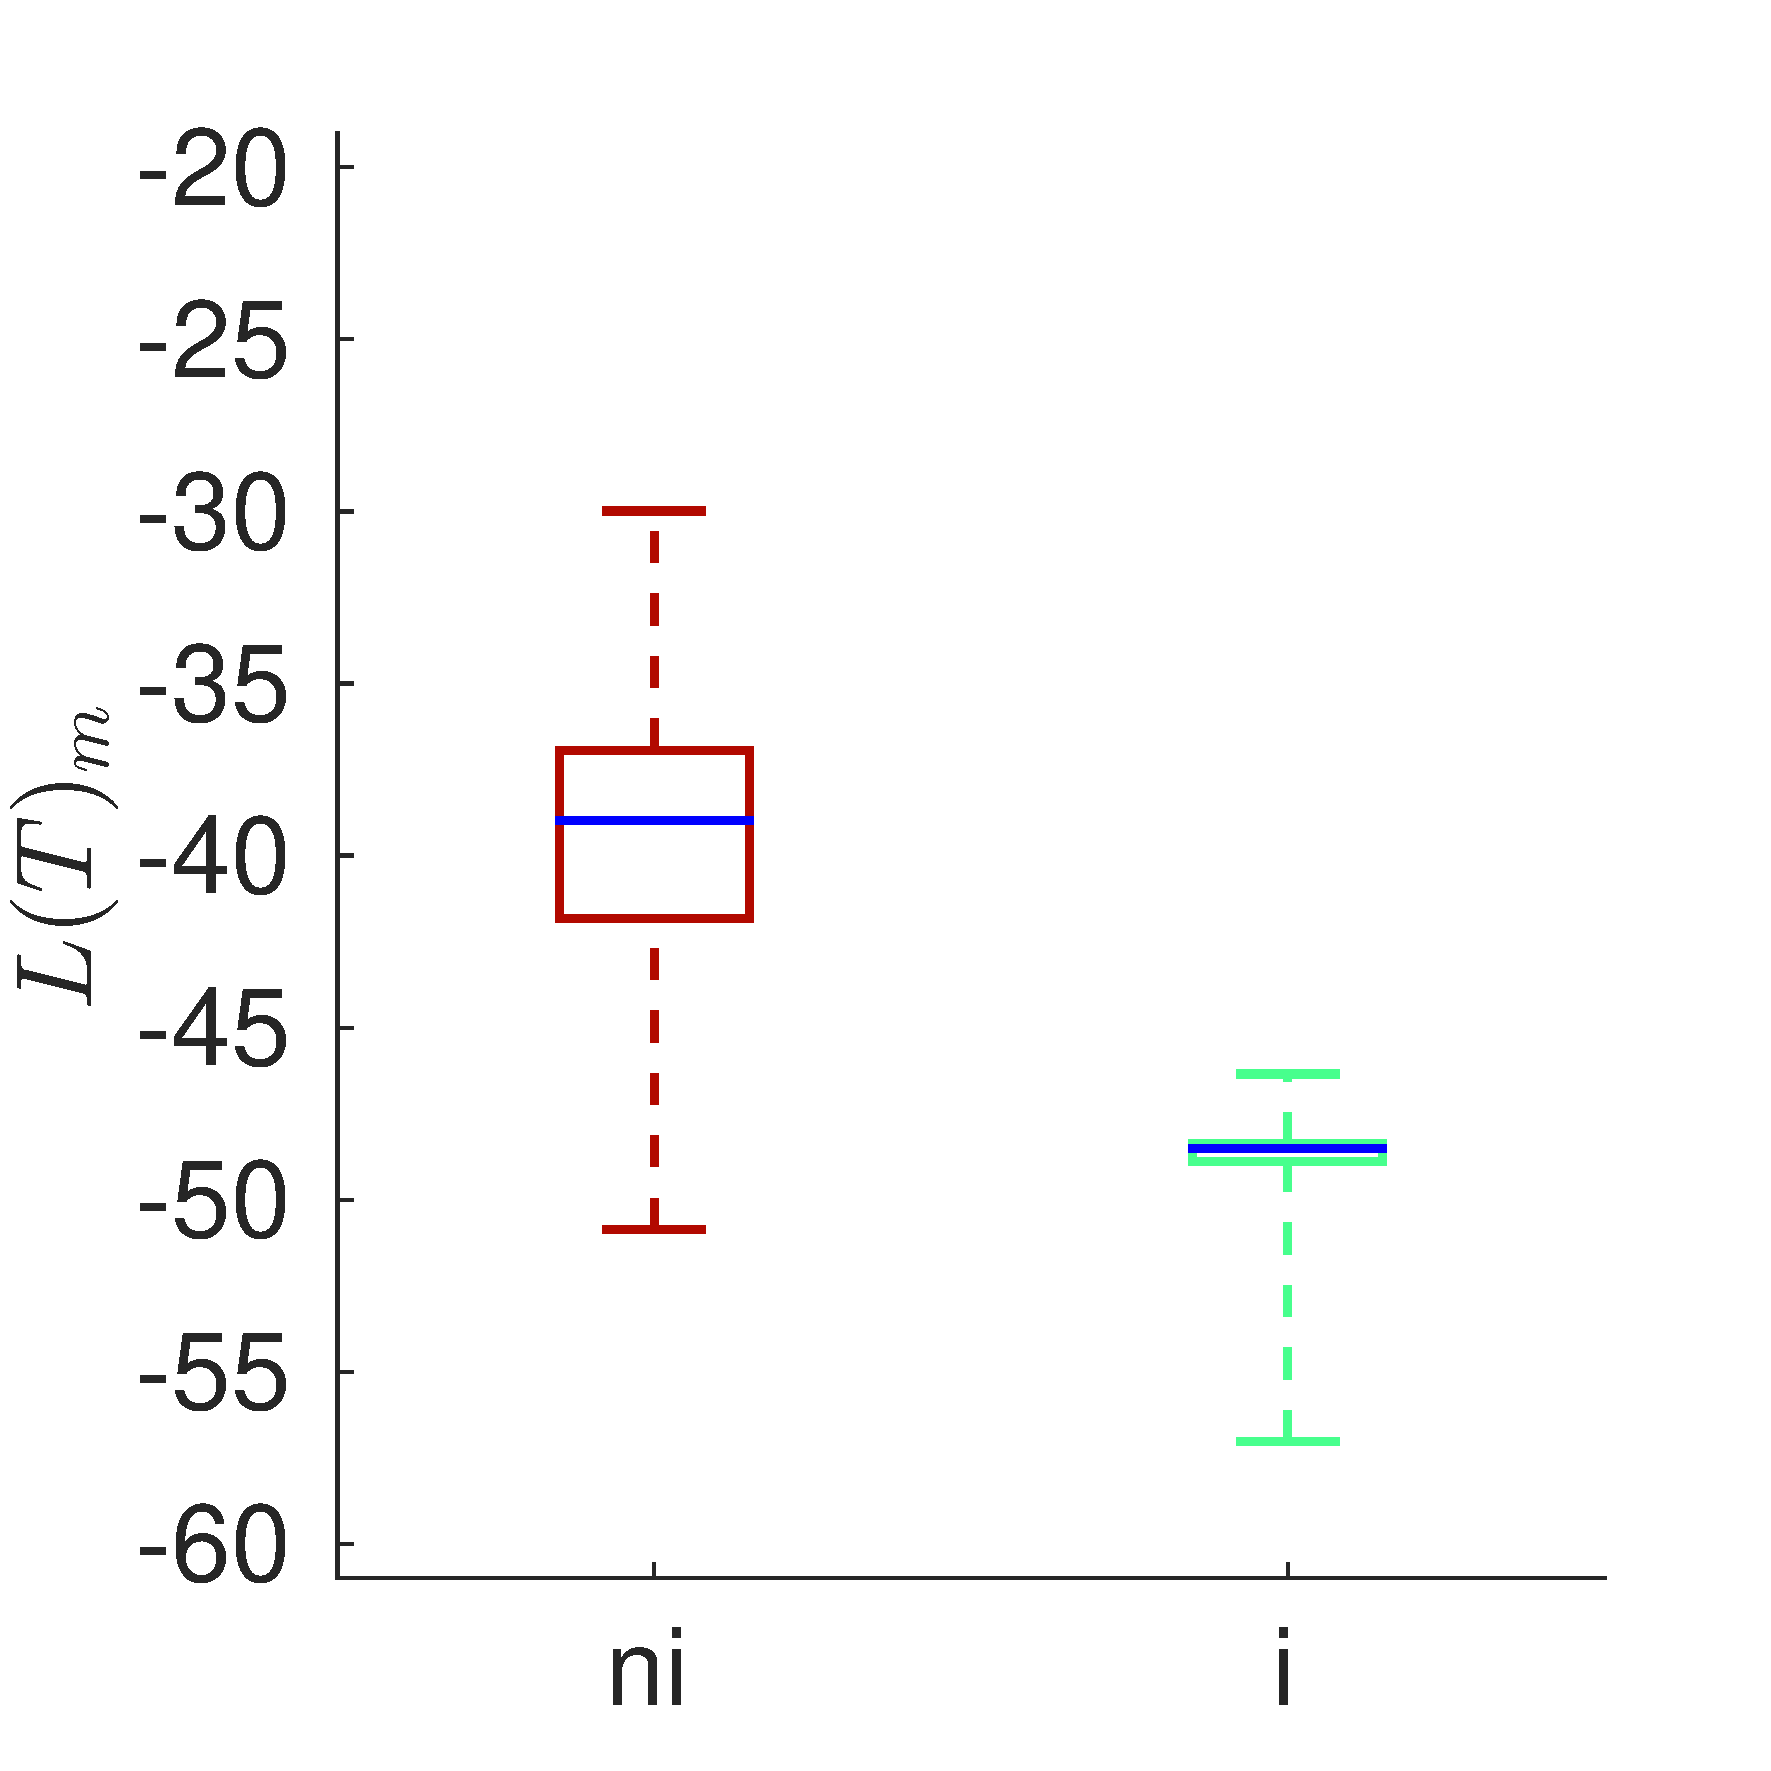
\includegraphics[width=.33\linewidth]{gfxXpUrbanSoundscape/xp_soundlevel_15}\label{fig:soundlevelMarkerc}}\par
        \subfloat[]
        {\includegraphics[width=.33\linewidth]{gfxXpUrbanSoundscape/xp_soundlevel_8}\label{fig:soundlevelMarkerd}}
        \subfloat[]
        {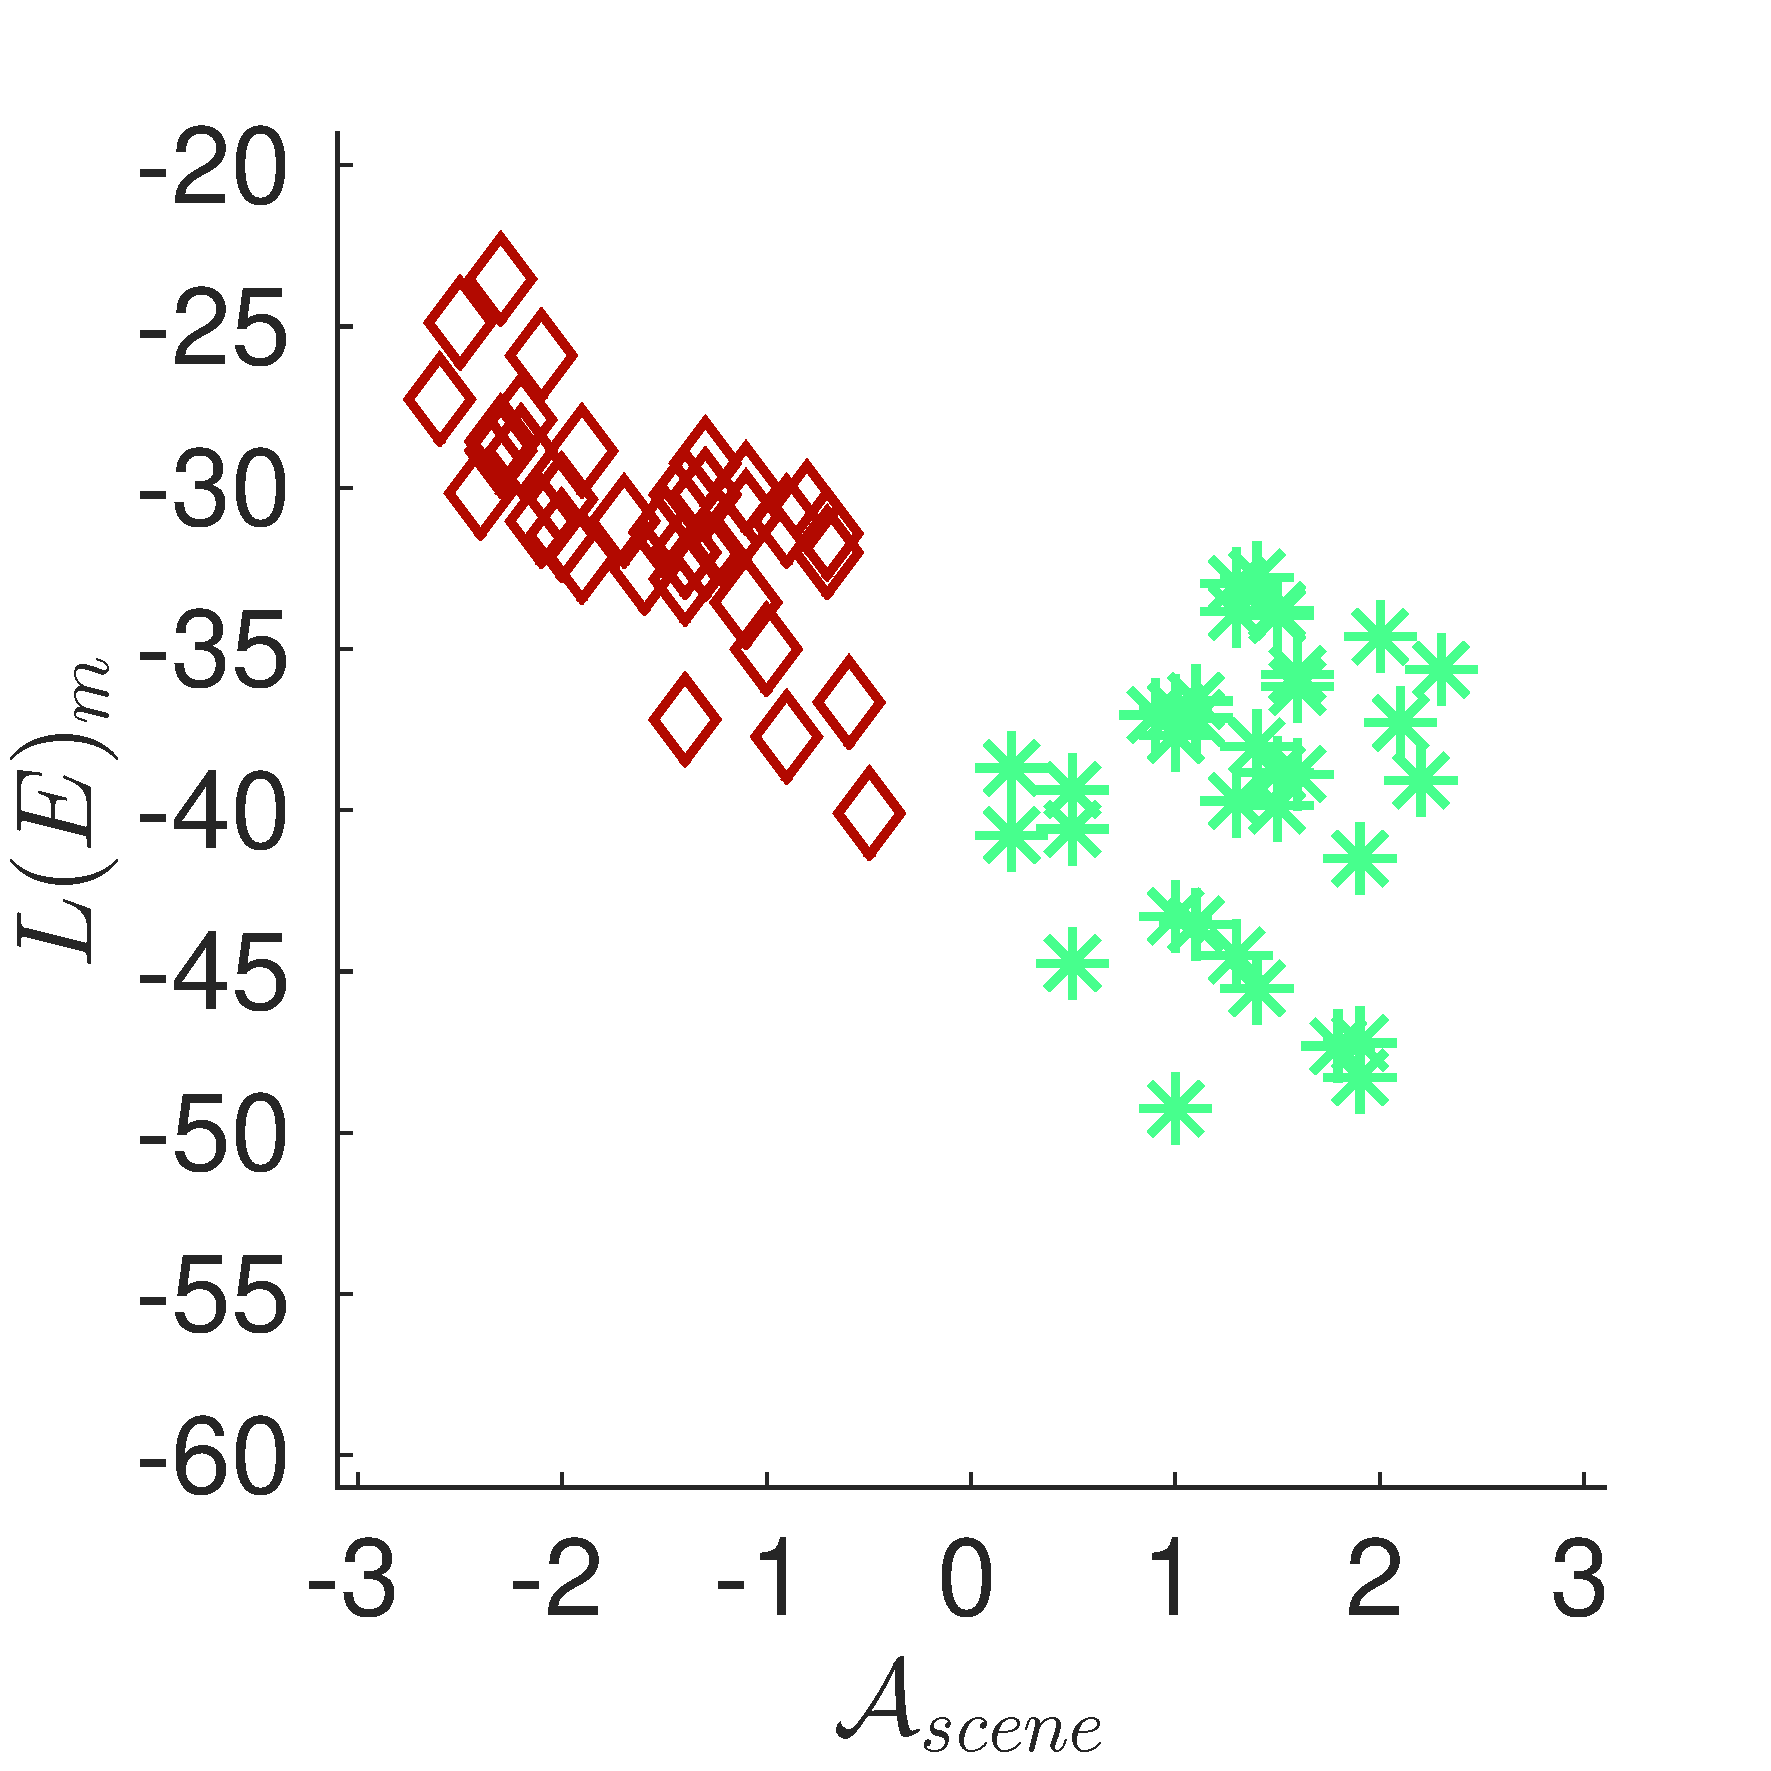
\includegraphics[width=.33\linewidth]{gfxXpUrbanSoundscape/xp_soundlevel_12}\label{fig:soundlevelMarkere}}
        \subfloat[]
        {\includegraphics[width=.33\linewidth]{gfxXpUrbanSoundscape/xp_soundlevel_16}\label{fig:soundlevelMarkerf}}       
        \caption[TODO]{TODO}\label{fig:soundlevelMarker}
\end{figure}

\begin{figure}[t]
        \myfloatalign 
        \subfloat[]
        {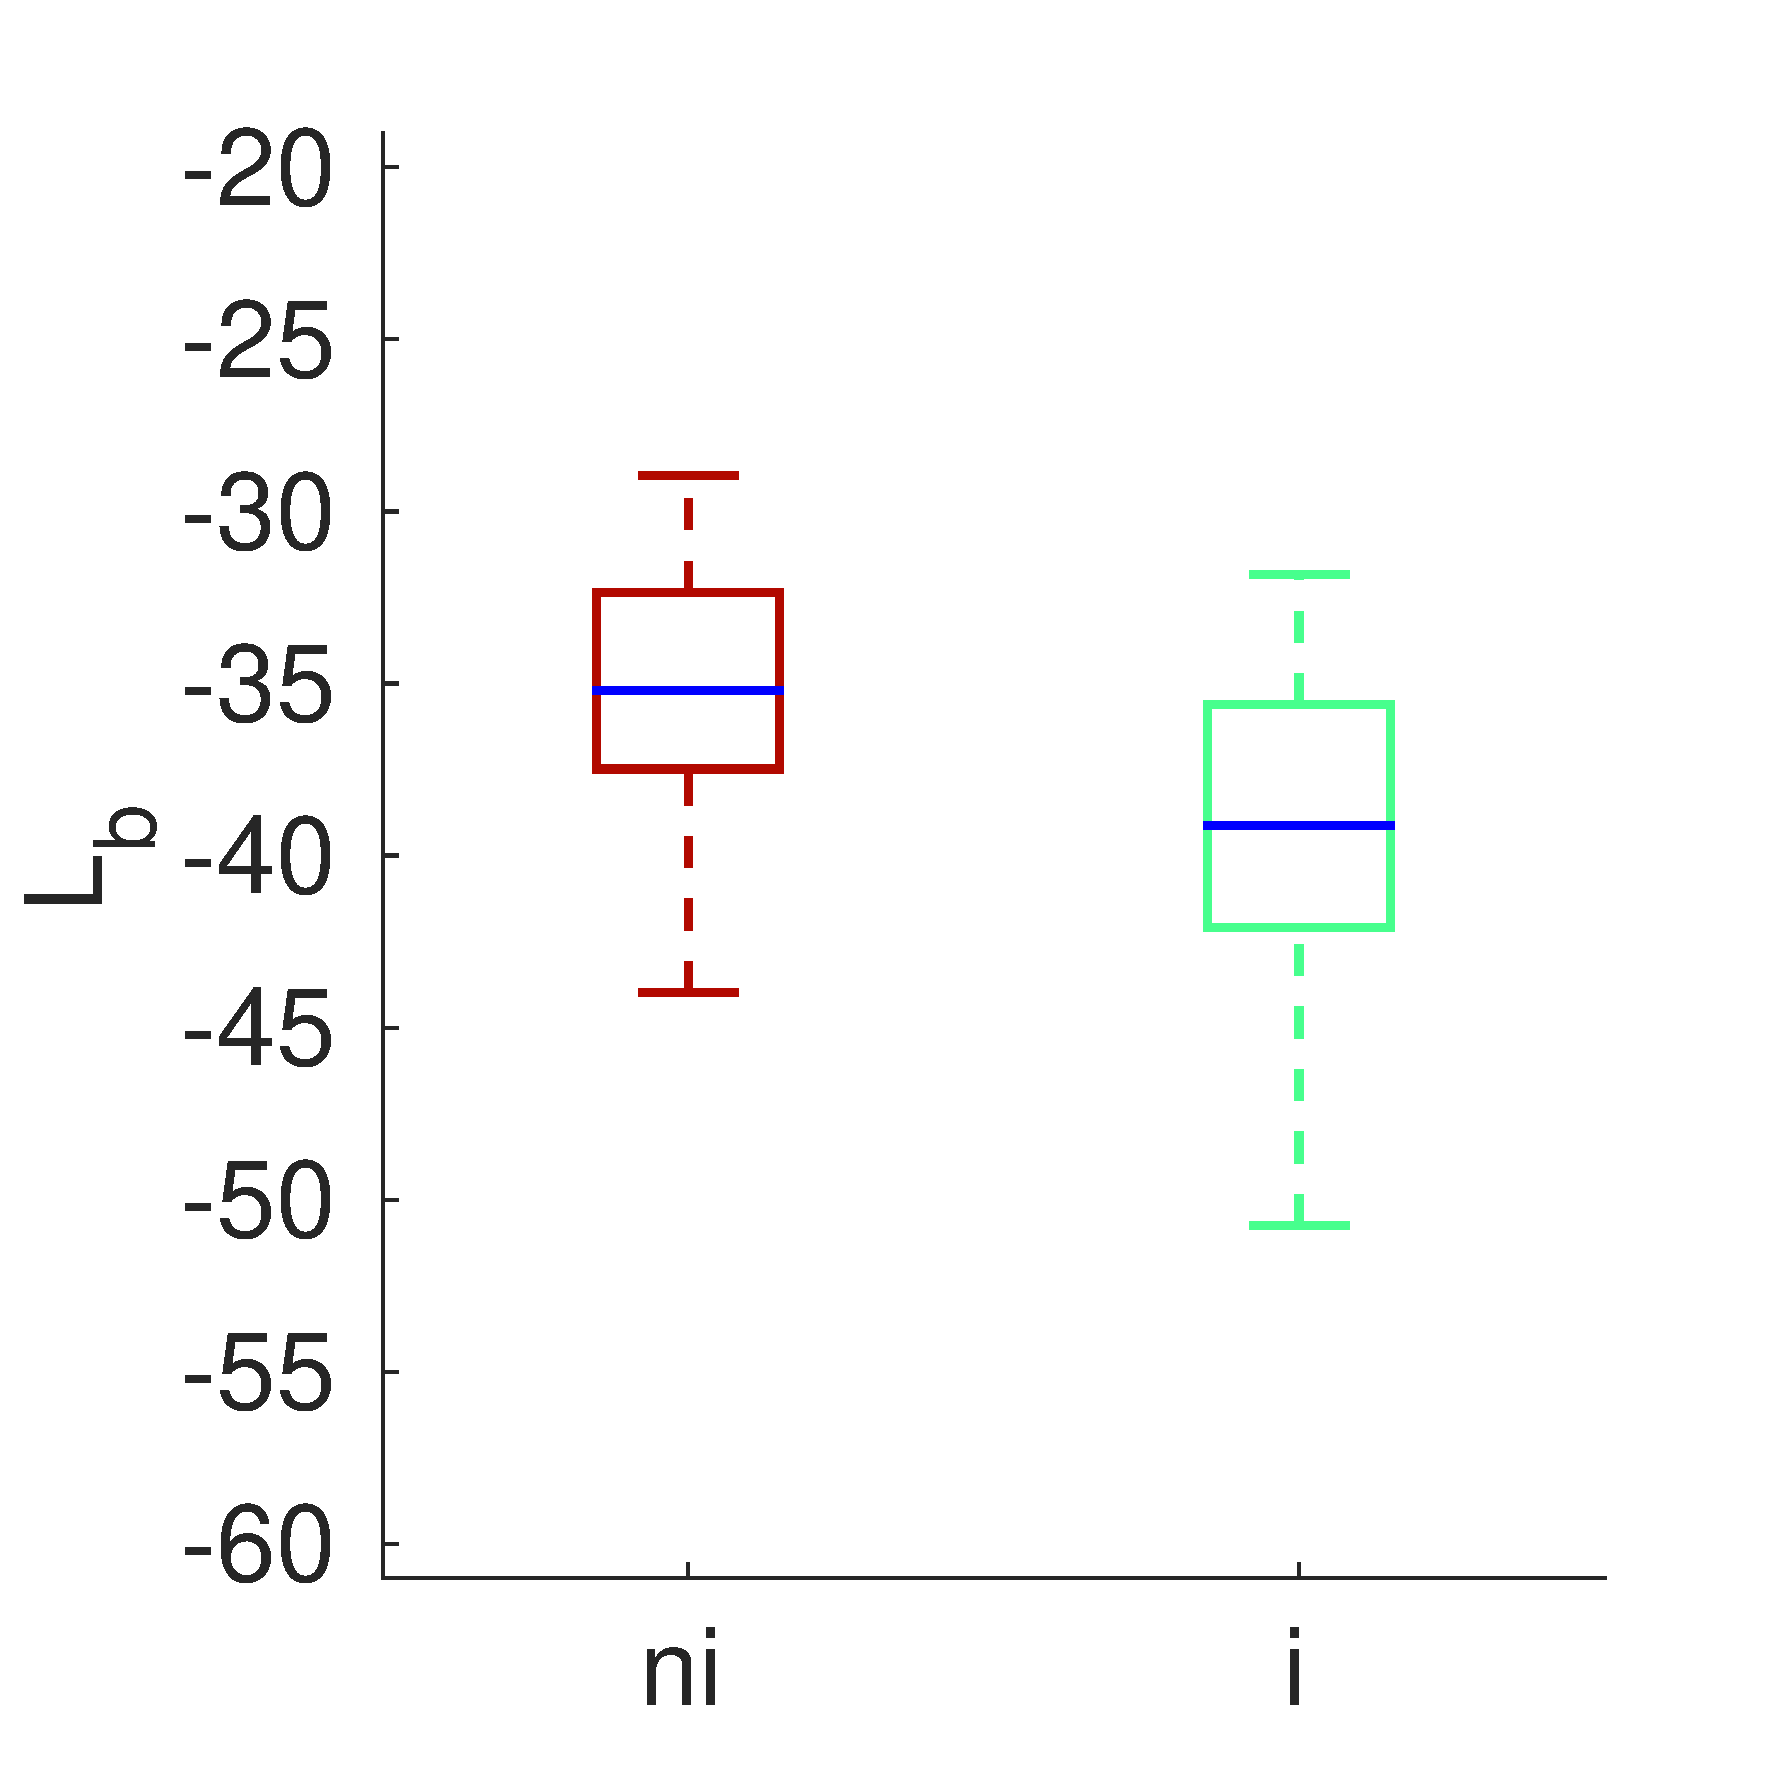
\includegraphics[width=.33\linewidth]{gfxXpUrbanSoundscape/xp_soundlevel_9}\label{fig:soundlevelNoisea}}
        \subfloat[]
        {\includegraphics[width=.33\linewidth]{gfxXpUrbanSoundscape/xp_soundlevel_13}\label{fig:soundlevelNoiseb}}
        \subfloat[]
        {\includegraphics[width=.33\linewidth]{gfxXpUrbanSoundscape/xp_soundlevel_17}\label{fig:soundlevelNoisec}}\par
        \subfloat[]
        {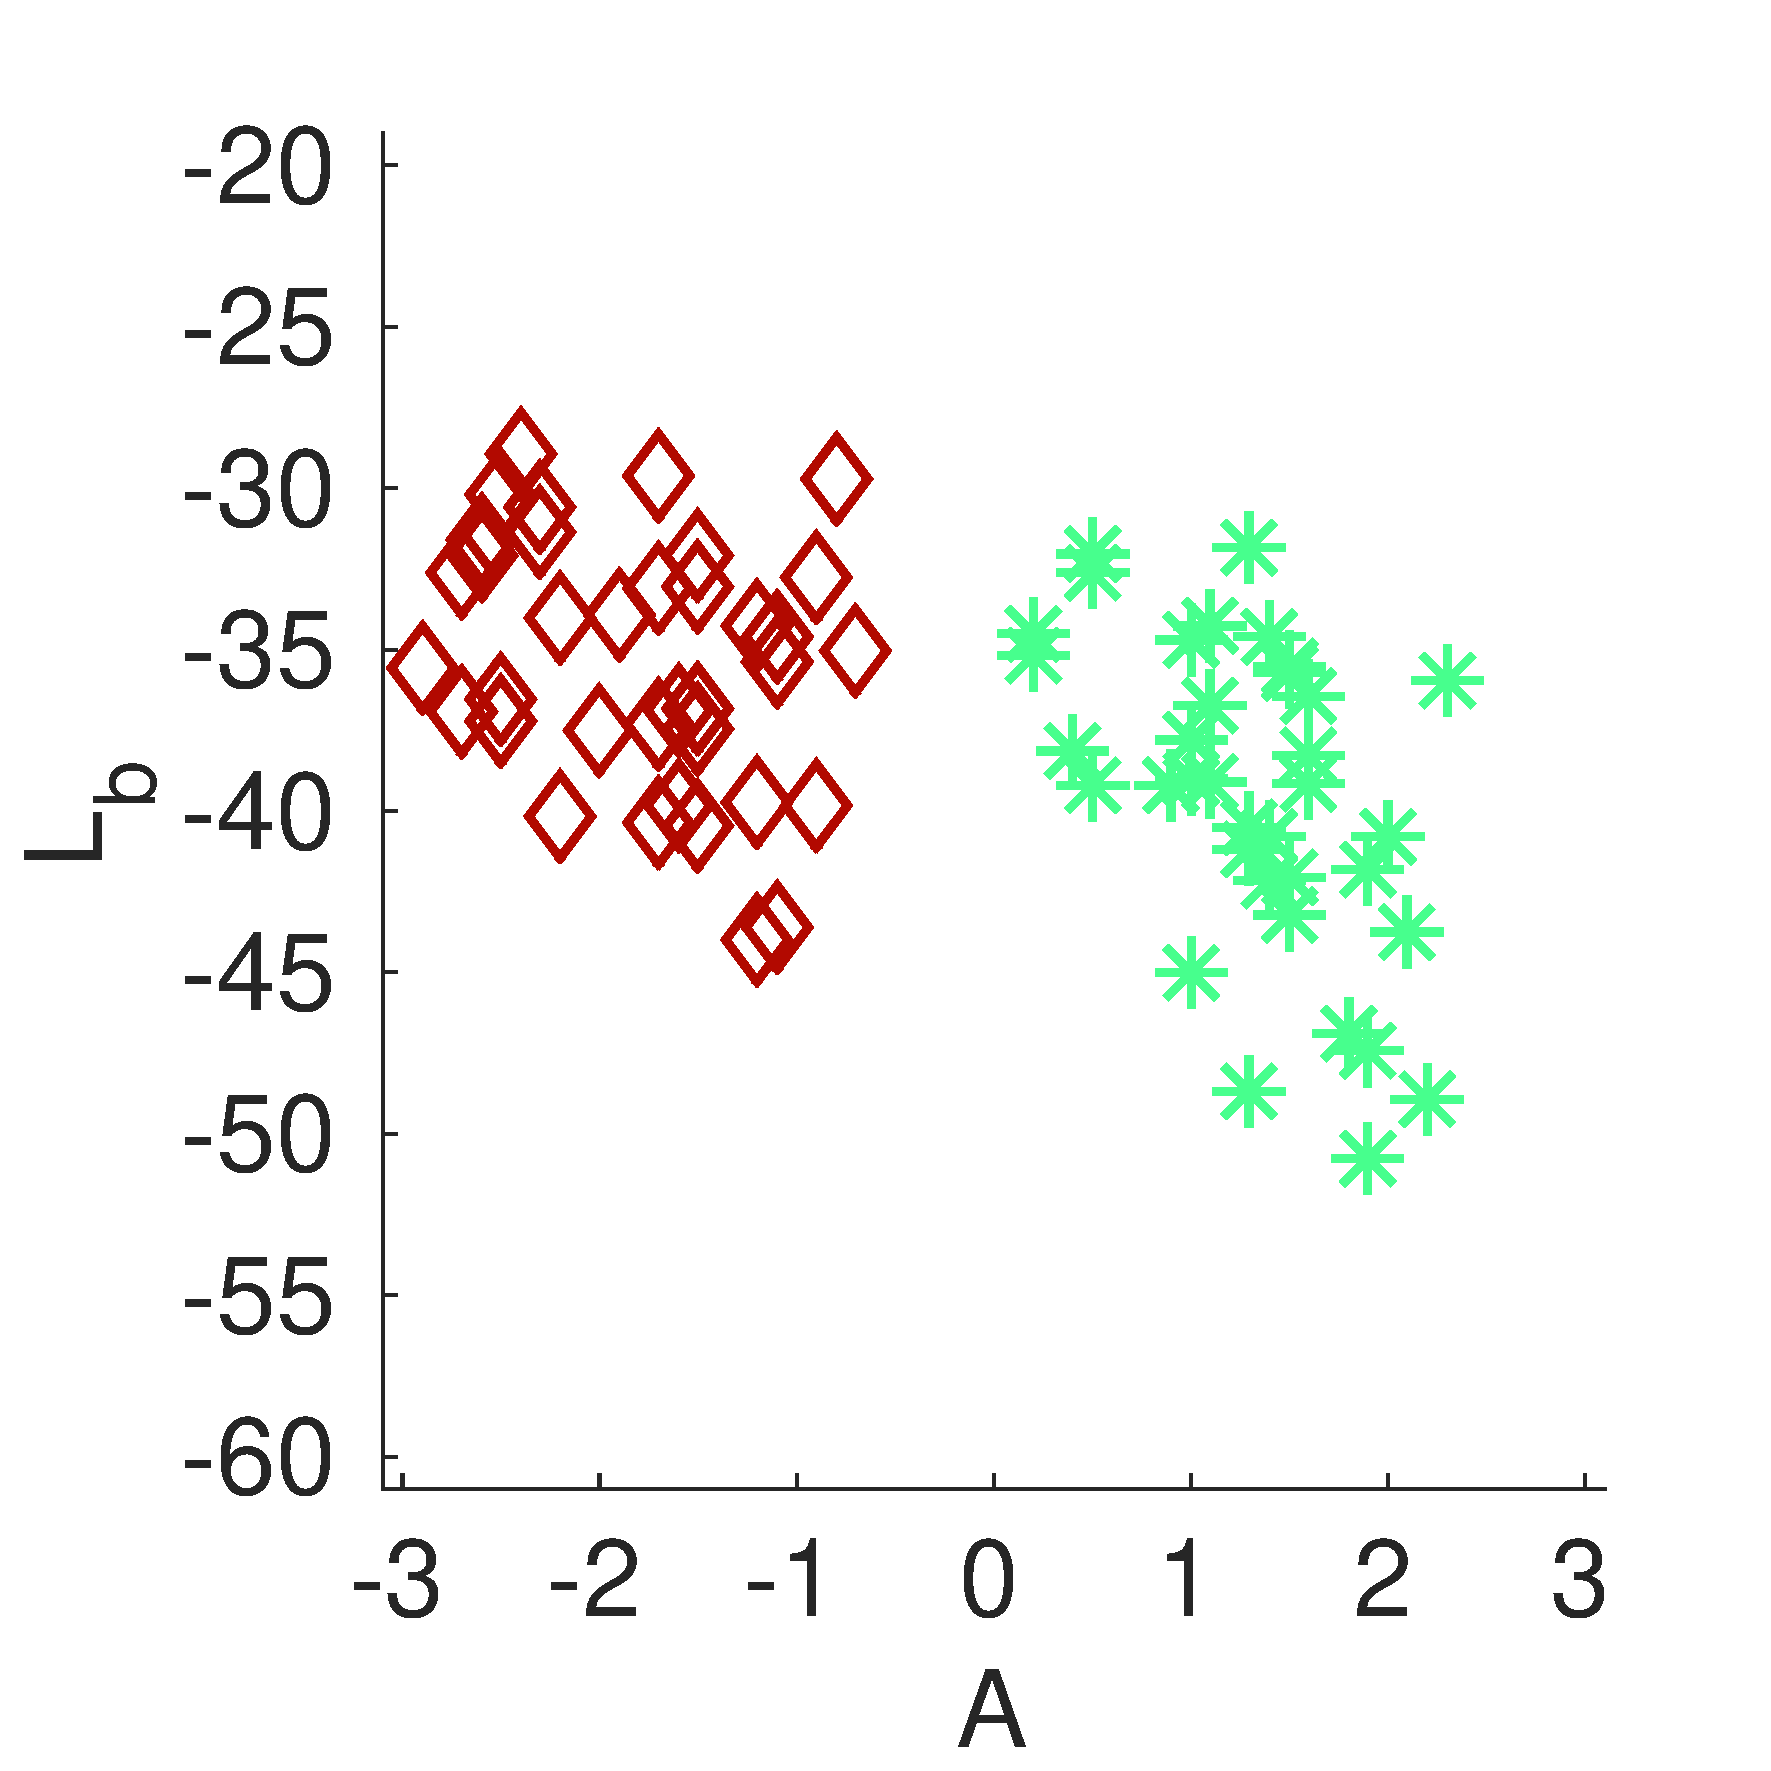
\includegraphics[width=.33\linewidth]{gfxXpUrbanSoundscape/xp_soundlevel_10}\label{fig:soundlevelNoised}}
        \subfloat[]
        {\includegraphics[width=.33\linewidth]{gfxXpUrbanSoundscape/xp_soundlevel_14}\label{fig:soundlevelNoisee}}
        \subfloat[]
        {\includegraphics[width=.33\linewidth]{gfxXpUrbanSoundscape/xp_soundlevel_18}\label{fig:soundlevelNoisef}}
       \caption[TODO]{TODO}\label{fig:soundlevelNoise}
\end{figure}

\begin{figure}[t]
        \myfloatalign 
        \subfloat[]
        {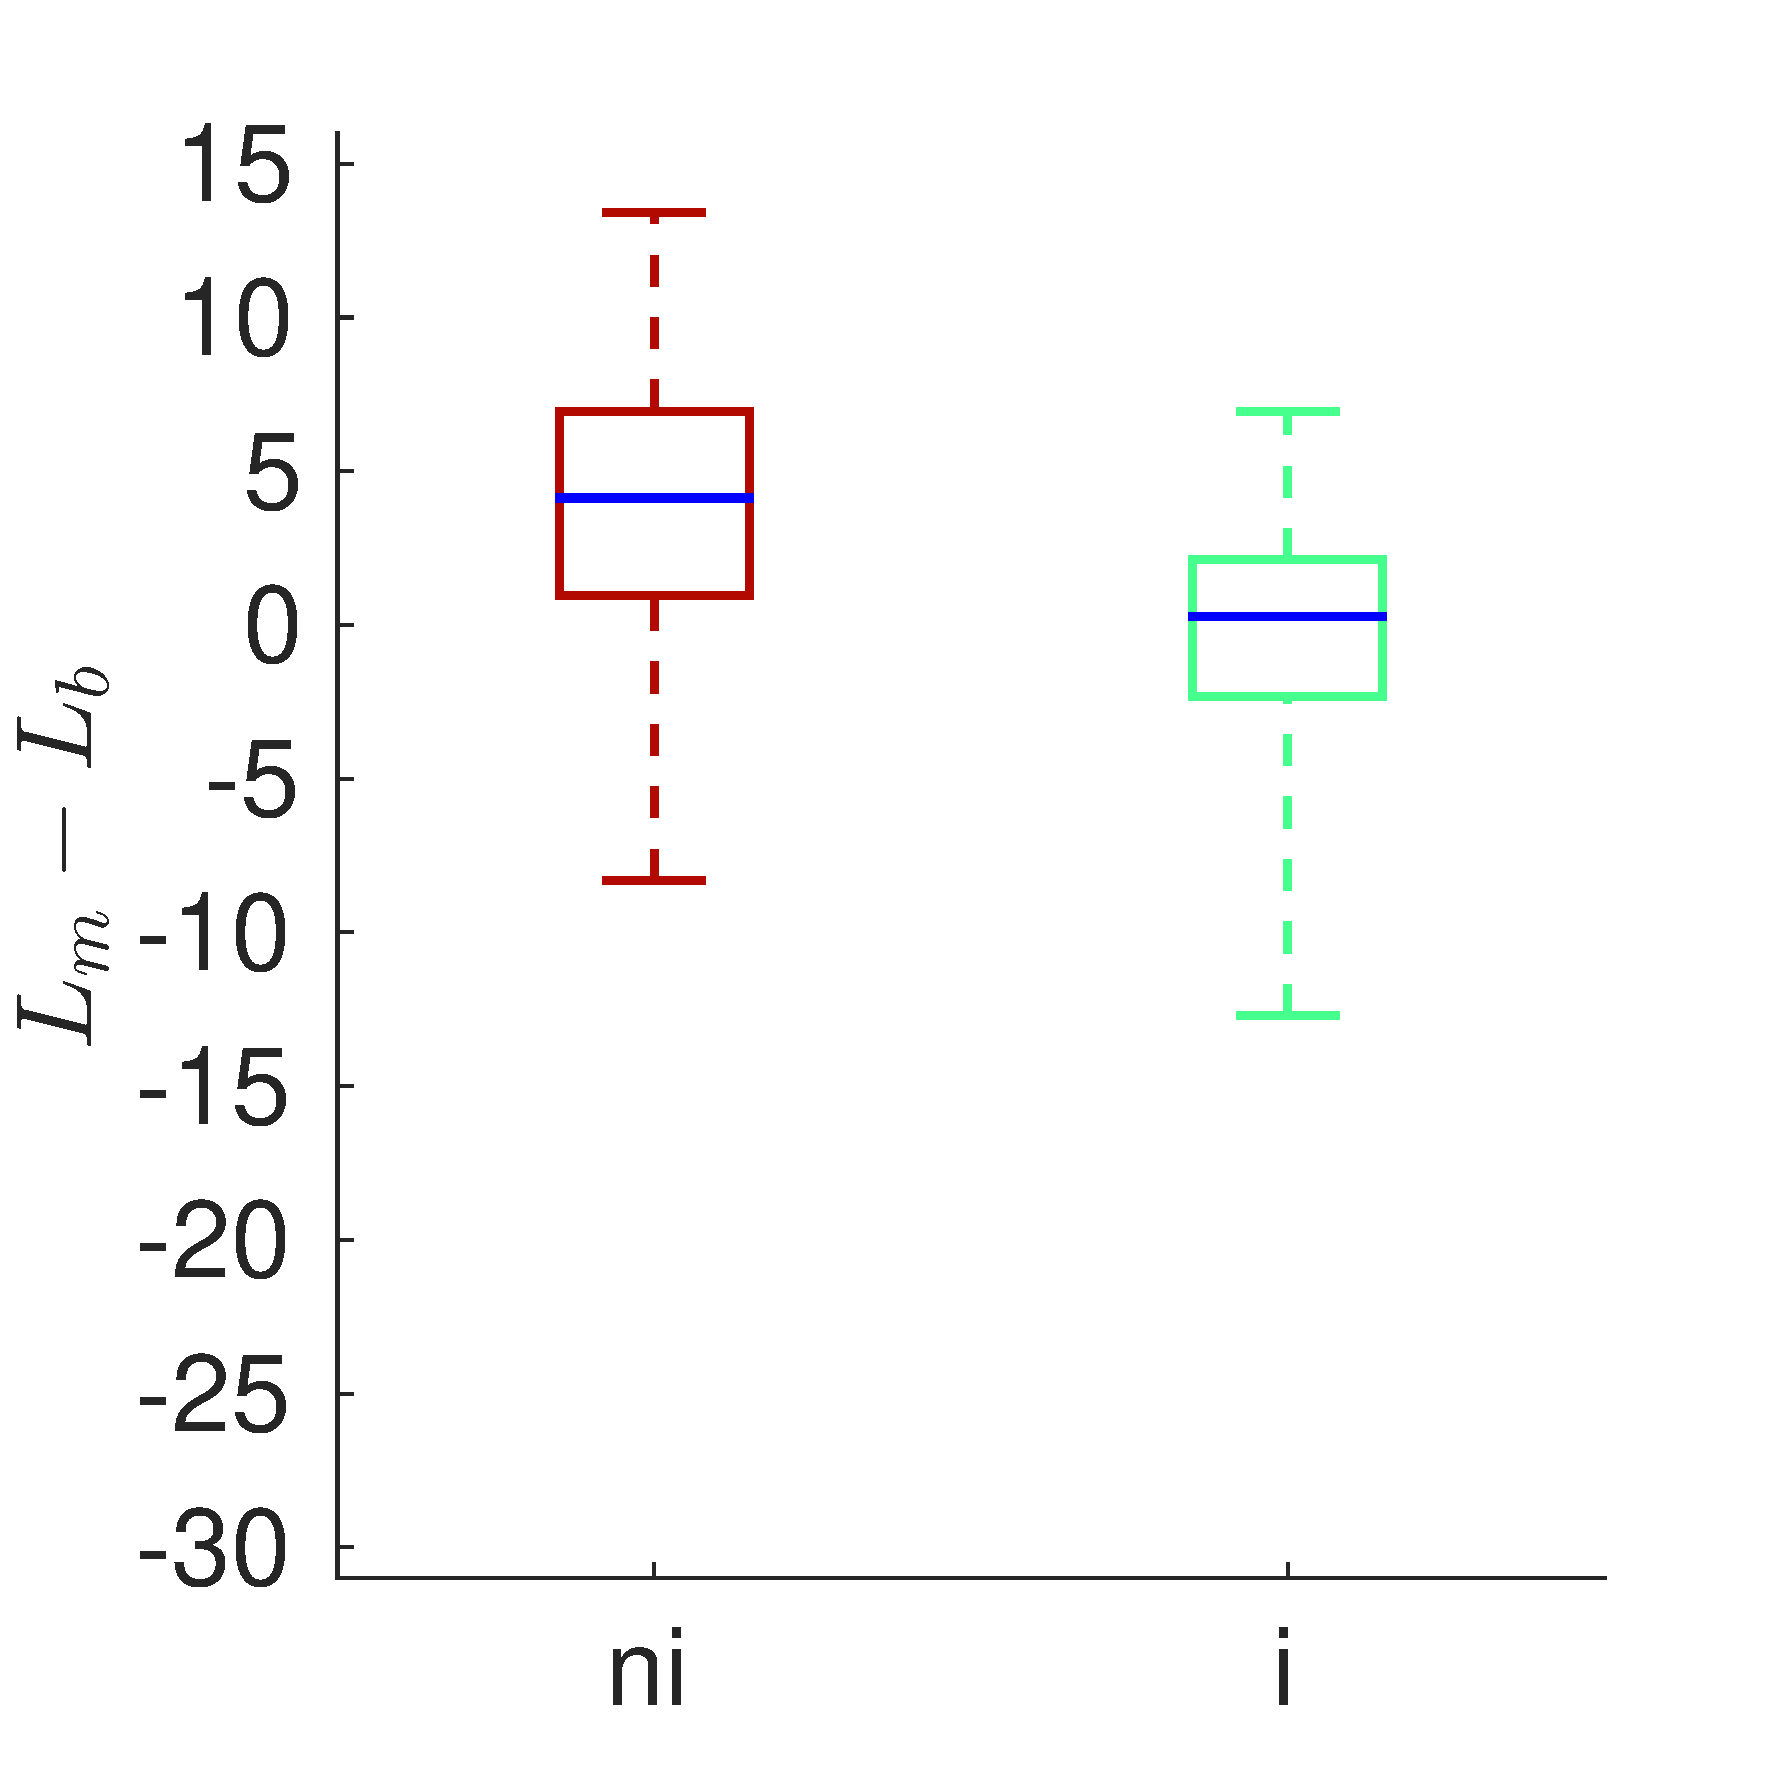
\includegraphics[width=.33\linewidth]{gfxXpUrbanSoundscape/xp_soundlevel_19}\label{fig:soundlevelMarkerDiffa}}
        \subfloat[]
        {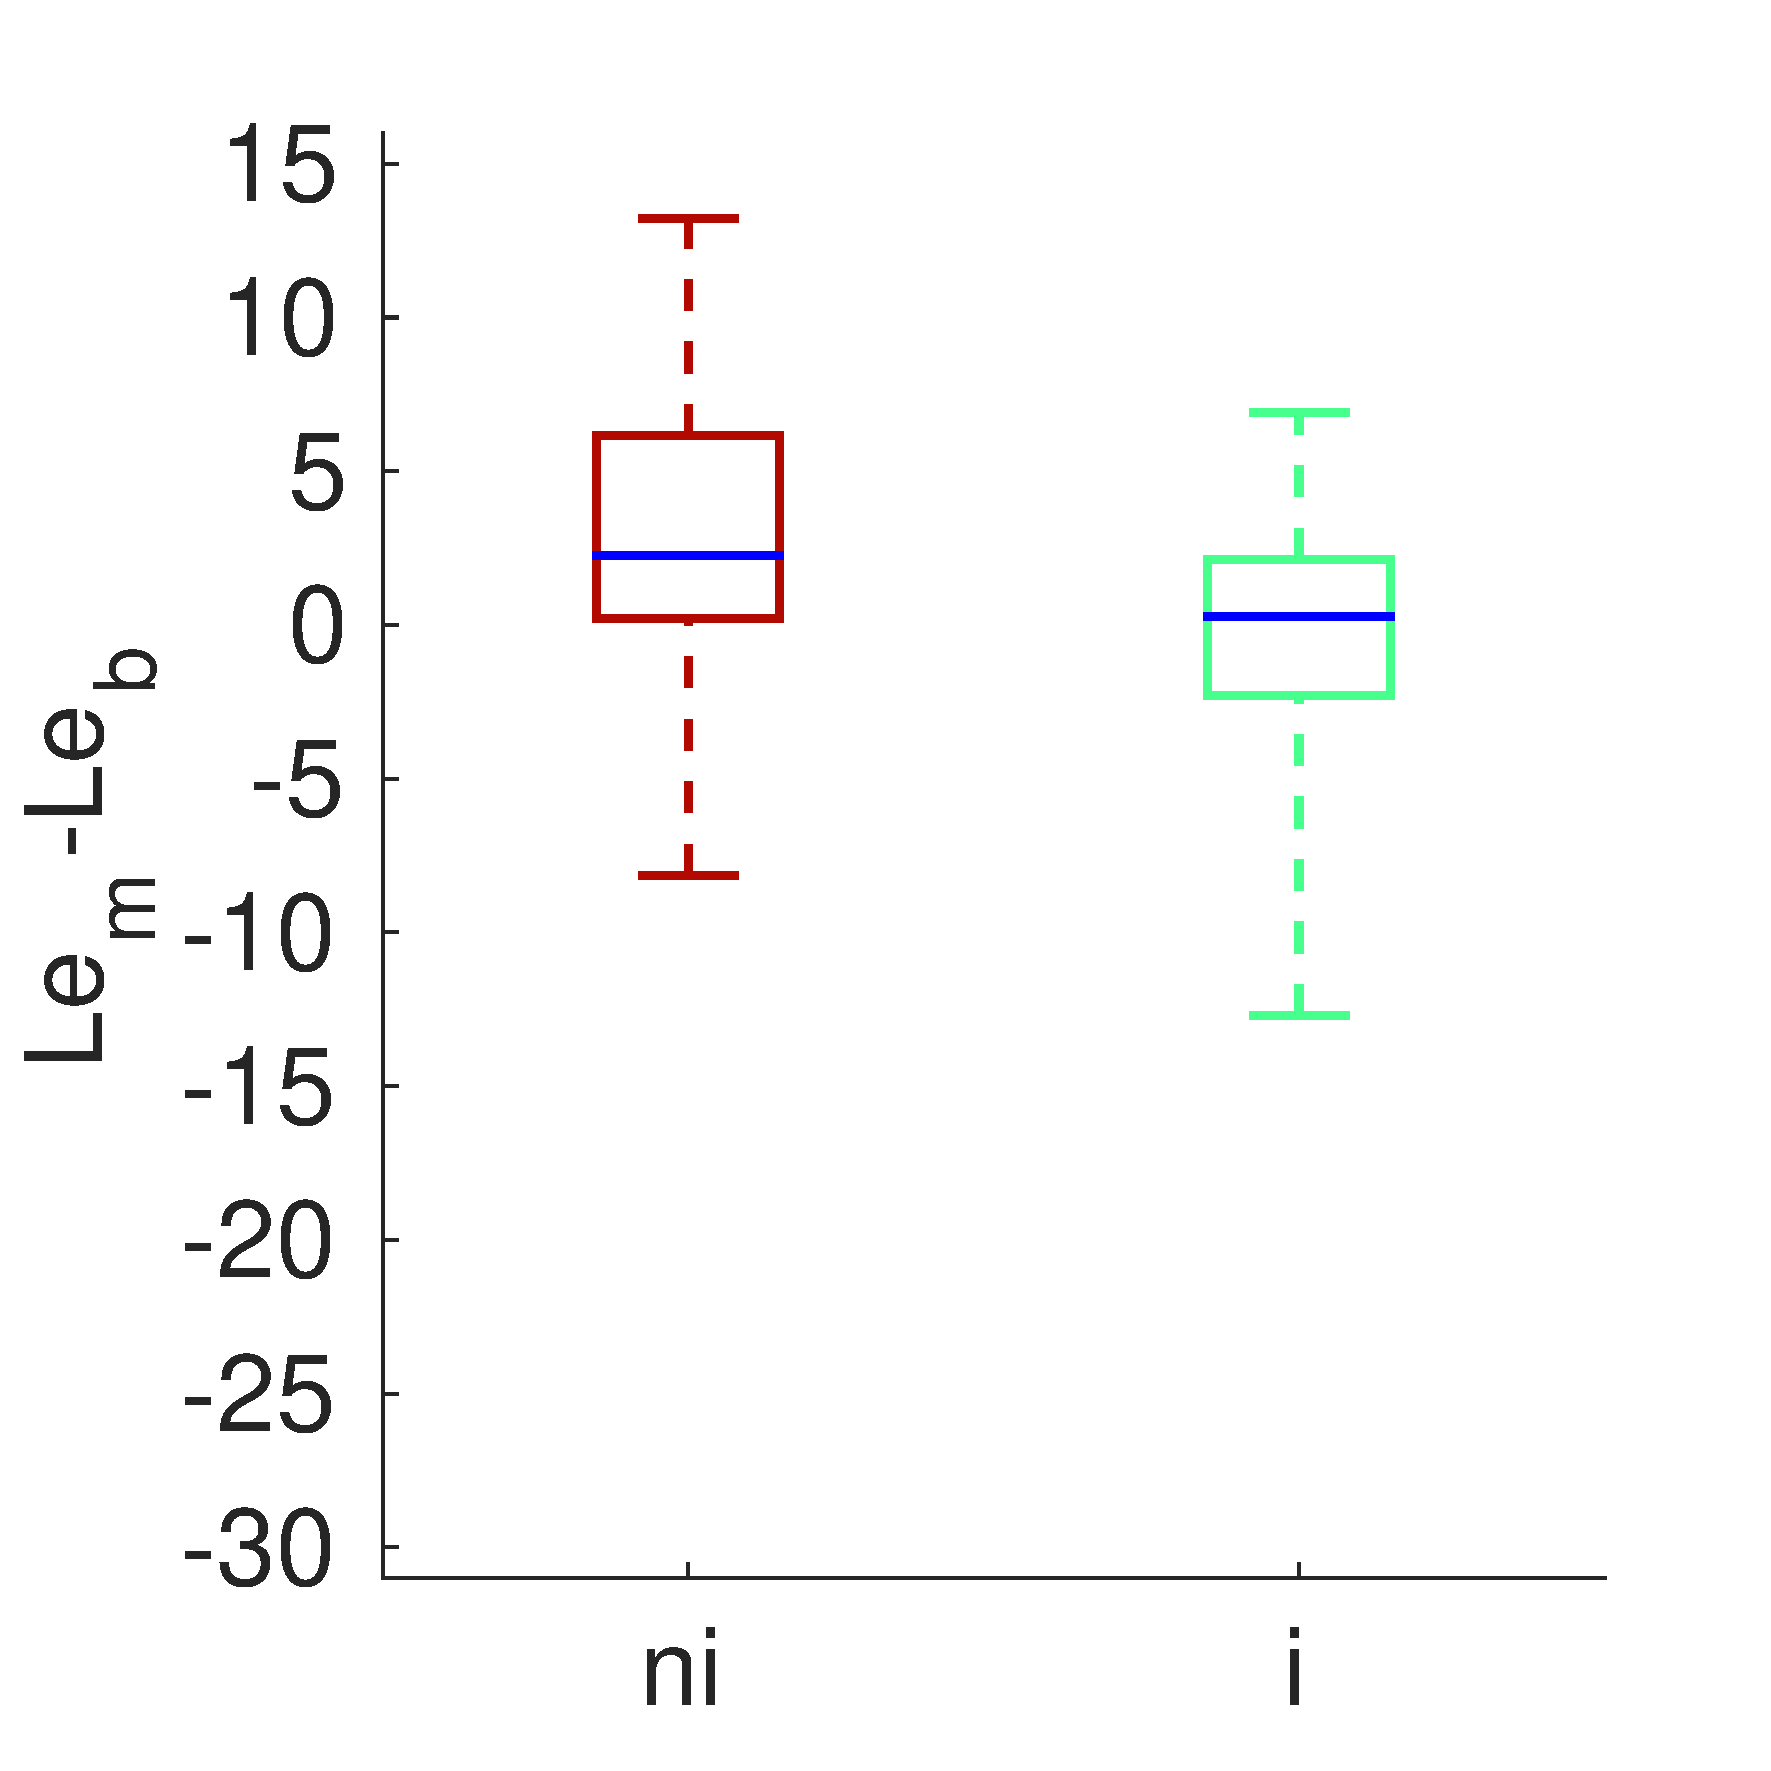
\includegraphics[width=.33\linewidth]{gfxXpUrbanSoundscape/xp_soundlevel_21}\label{fig:soundlevelMarkerDiffb}}
        \subfloat[]
        {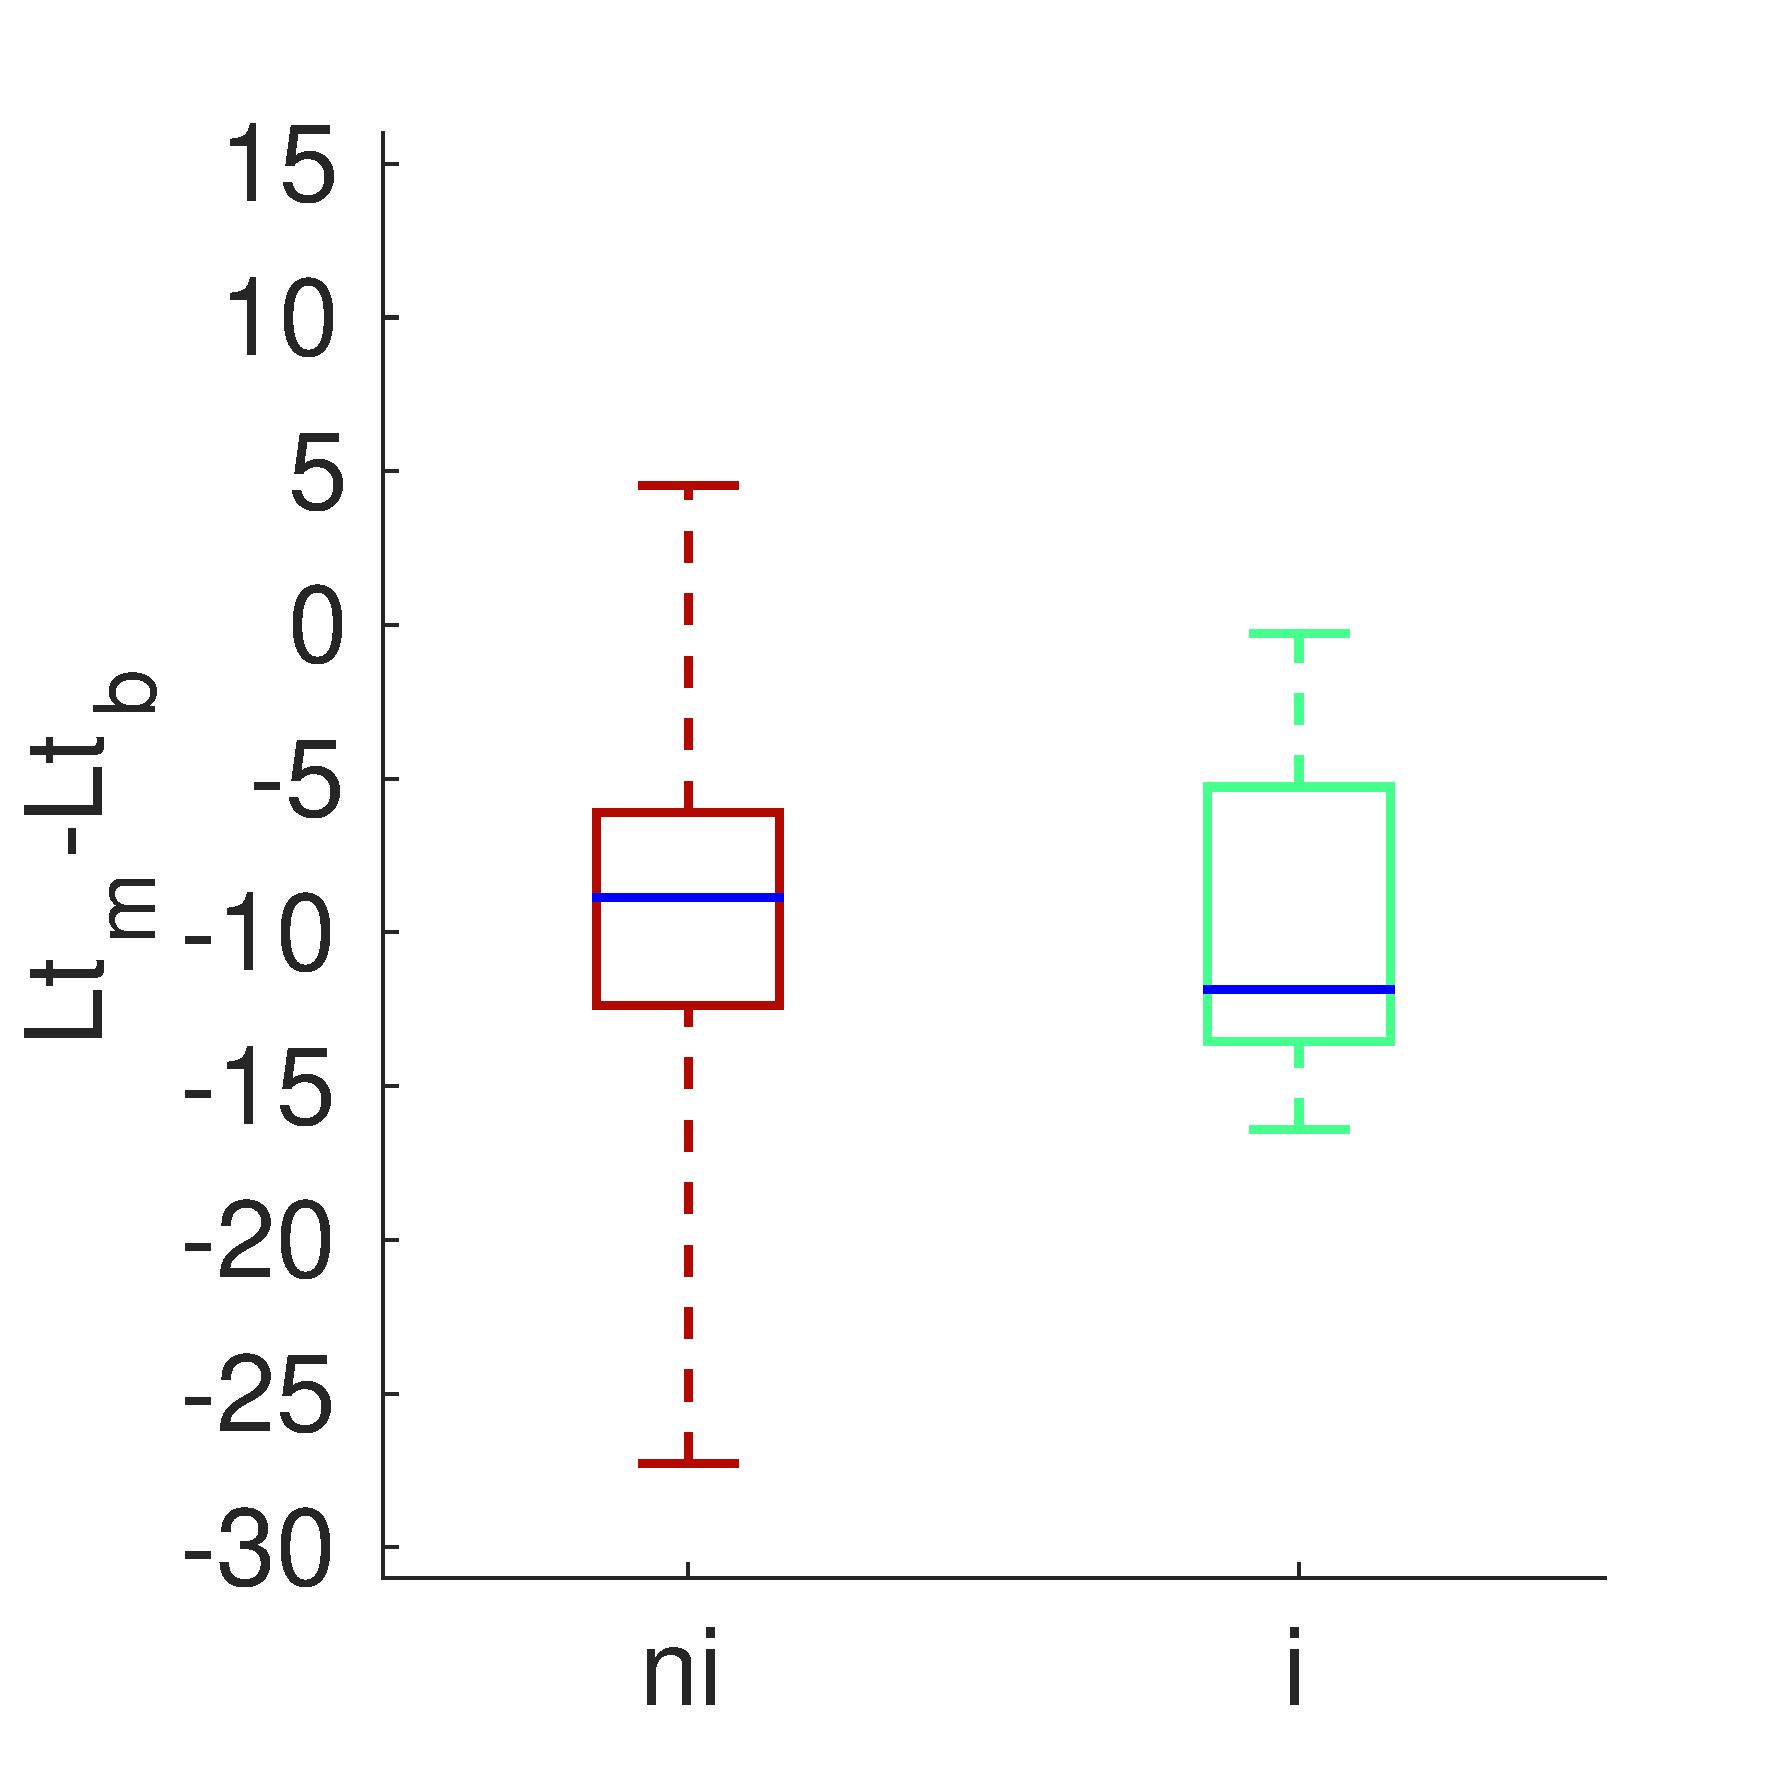
\includegraphics[width=.33\linewidth]{gfxXpUrbanSoundscape/xp_soundlevel_23}\label{fig:soundlevelMarkerDiffc}}\par
        \subfloat[]
        {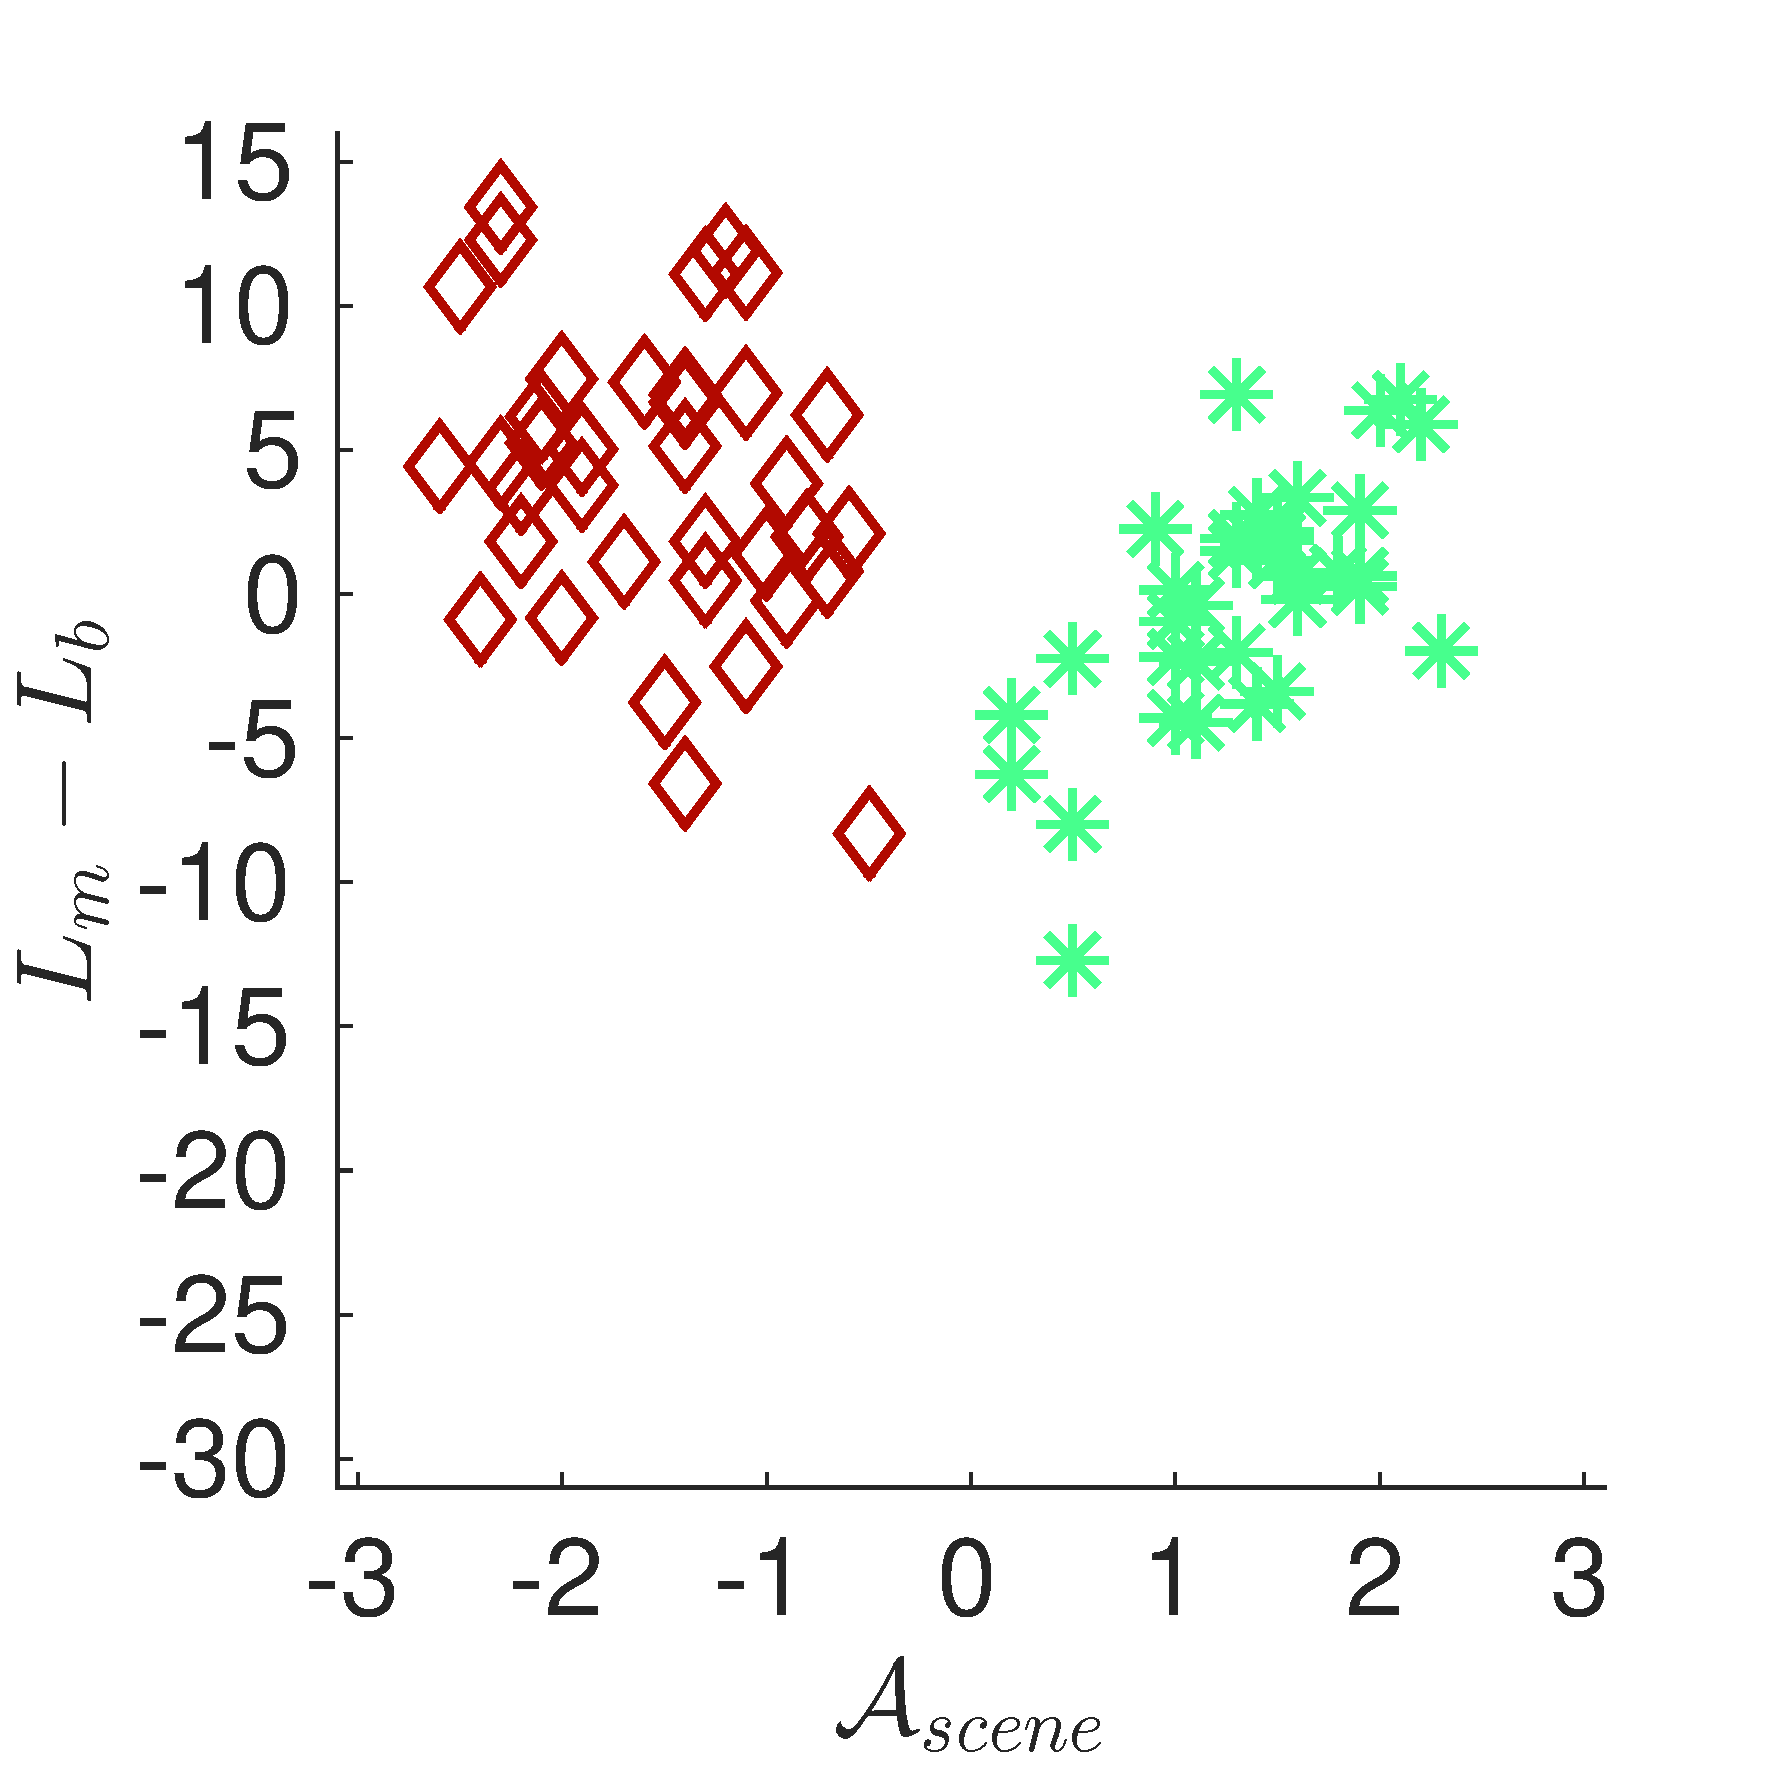
\includegraphics[width=.33\linewidth]{gfxXpUrbanSoundscape/xp_soundlevel_20}\label{fig:soundlevelMarkerDiffd}}
        \subfloat[]
        {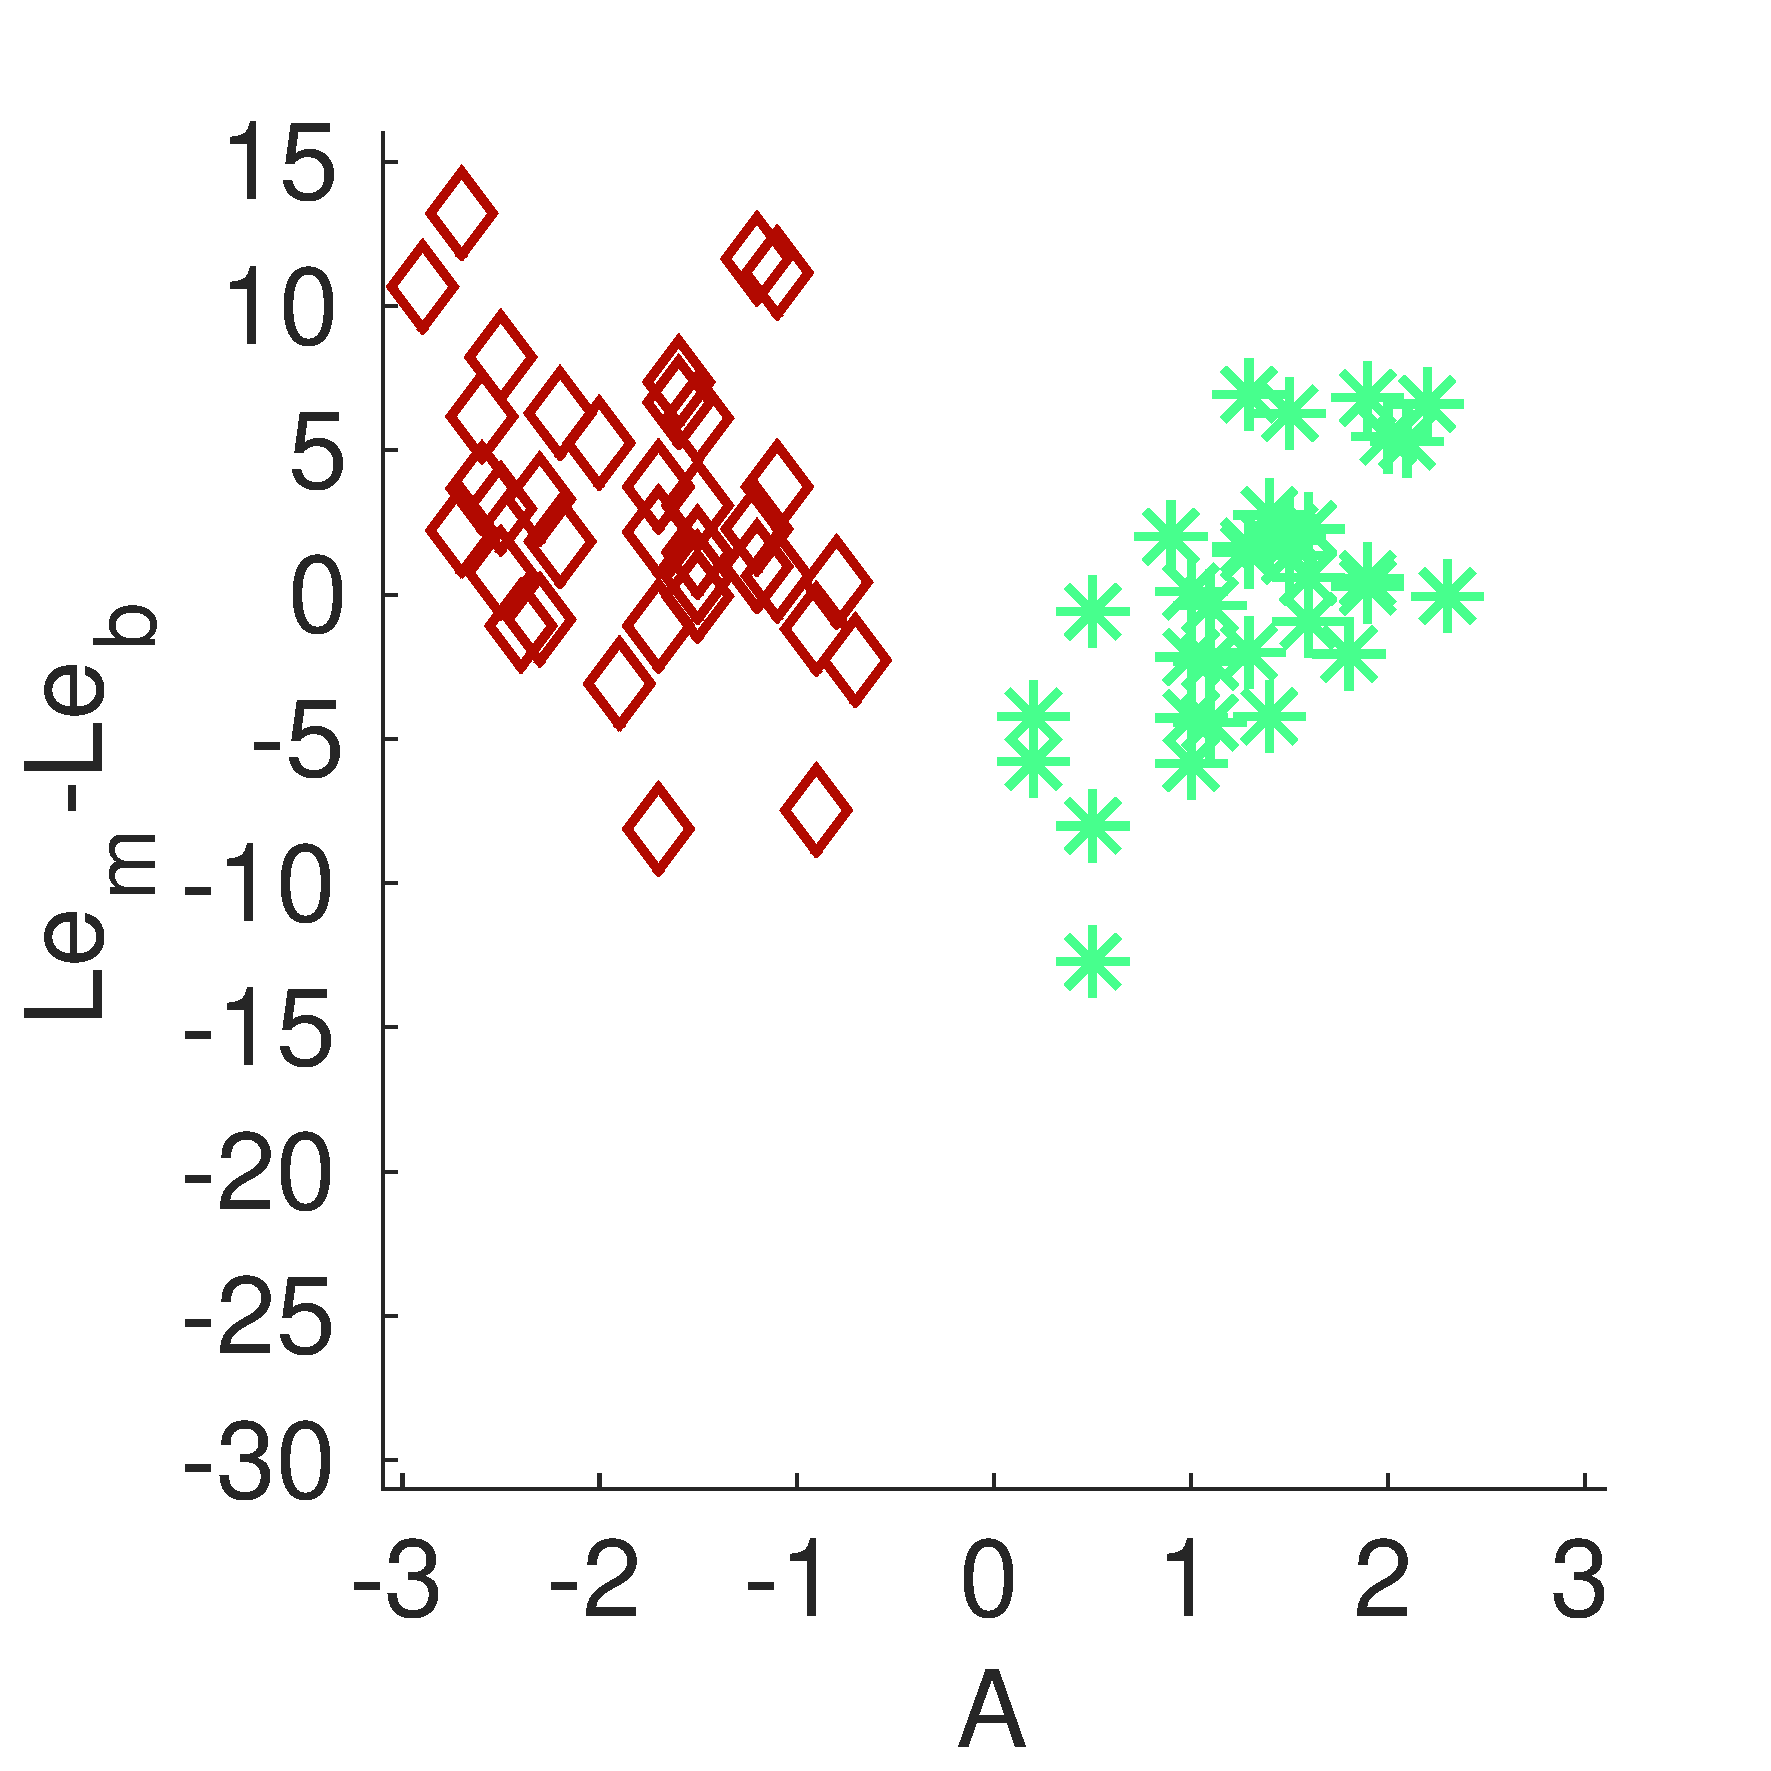
\includegraphics[width=.33\linewidth]{gfxXpUrbanSoundscape/xp_soundlevel_22}\label{fig:soundlevelMarkerDiffe}}
        \subfloat[]
        {\includegraphics[width=.33\linewidth]{gfxXpUrbanSoundscape/xp_soundlevel_24}\label{fig:soundlevelMarkerDifff}}
       \caption[TODO]{TODO}\label{fig:soundlevelMarkerDiff}
\end{figure}




\subsection{Discussions}

Dans cette expérience, nous identifions 6 indicateurs structurels globaux permettant de distinguer, de manière globale, les environnements sonores idéaux et non-idéaux.

\begin{itemize}
\item niveau sonore: calculé sur tous les sons $L$, les événements $L(E)$ et les textures $L(T)$; 
\item densité: calculée de manière globale $D$ et sur les événements $D(E)$;
\item diversité: calculée uniquement sur les événements $DIV(E)$.
\end{itemize}

Parmi ces indicateurs structurels, seuls $L$ et $LE$ permettent de prédire l'agrément. Nous notons cependant que cette prédiction ne vaut que pour les ni-scènes. 

Nous observons qu'une description sémantique des scènes, basée sur la présence/absence des classes de sons, permet de bien prédire la nature de l'environnement. Par ailleurs, il apparaît qu'il est possible d'obtenir une prédiction similaire, voire meilleure, en ne considérant qu'un sous groupe de classes d'événements,\ie~les marqueurs sonores.

Parmi les descripteurs structurels spécifiques, calculés en tenant compte des marqueurs sonores, plusieurs permettent maintenant de faire la distinction entre les i-scènes et ni-scènes:

\begin{itemize}
\item \gl{TODO}.
\end{itemize}

Parmi ces descripteurs, 8 semblent impacter l'agrément perçu: 

\begin{itemize}
\item $L_b$ et $L(E)_b$ ont un impact négatif sur les i-scènes;
\item $L(E)_m-L(E)_b$ et $L_m-L_b$ ont un impact positif sur les i-scènes;
\item $L_m$, $L(E)_m$, $L(T)_b$ et $D(E)_m$ ont un impact négatif les ni-scènes.
\end{itemize}

De cette analyse, nous retenons les points suivants:

\begin{itemize}
\item \emph{distinguer les i- et ni-scènes}: Les descripteurs sémantiques, ainsi que certains descripteurs structurels globaux, permettent de faire la distinction entre les i-scènes et les ni-scènes. La description sémantique semble être plus performante;
\item \emph{événements ou textures}: Que ce soit pour les descripteurs sémantiques ou structurels, c'est majoritairement les événements qui permettent de distinguer les deux types d'environnements, les textures n'apportant, au mieux, qu'une information limitée;
\item \emph{prédire l'agrément}: Si l'on considère une description fine de l'agrément, il semble que la manière de percevoir la qualité de l'environnement diffère en fonction de la nature de ce dernier (i ou ni). Il n'apparaît pas envisageable de considérer un même jeu de descripteurs pour prédire, à la fois, l'agrément des i-scènes, et l'agrément des ni-scènes. Pour les ni-scènes, ce sont le niveau global ($L$ et $L(E)$), la densité globale ($D$ et $D(E)$), et/ou le niveau des marqueurs sonores ($L_m$ et $L$), qui impactent négativement l'agrément. On note ici que prendre en compte les contributions de différentes sources n'améliore pas la capacité de prédiction de l'agrément, par rapport à une analyse holistique de l'environnement. Pour les i-scènes, par contre, prédire l'agrément requiert d'étudier, de manière séparée, les caractéristiques des marqueurs sonores, et celles de l'ensemble des autres sons. Ainsi, le niveau des marqueurs relatifs au bruit est positivement corrélé à l'agrément, alors que le niveau du bruit est, lui, négativement corrélé.  
\end{itemize}

L'existence de deux modes de perception, mobilisant différents types de descripteurs, et dépendant de la nature du stimuli, est un phénomène qui a déjà été observé pour la perception des textures (\cf~Section~\ref{sec:ch3_eventTexture}). Le cerveau adapte sa manière de traiter l'information (résumé statistique pour les textures, description fine pour les événements) suite à une prise de décision antérieure quant à la nature du stimuli (à savoir ``\,est-ce un événement ou une texture ?\,''). De la même manière, les indicateurs actifs dans le jugement de l'agrément dépendent, eux aussi, d'une identification préalable de la nature hédonique globale de l'environnement (idéale ou non idéale).

Ces résultats peuvent potentiellement influer sur les stratégies à adopter pour améliorer la qualité de l’environnement sonore:

\begin{itemize}
\item dans le cadre de scènes non-idéales, il s'agit de diminuer le niveau sonore, soit de manière globale, soit en agissant sur certaines sources (\emph{sirène}, \emph{klaxon});
\item dans le cadre de scènes idéales, il s'agit 1) d'identifier les sons agréables, \ie~les marqueurs sonores, 2) de baisser le niveau des autres sons, 3) voire, en restant dans la limite du raisonnable, d'augmenter le niveau des marqueurs par rapport aux autres sons.
\end{itemize}

Nous montrons que les descripteurs à utiliser dépendent de la nature de l'environnement, et que cette nature est elle même dépendante de la composition sémantique, \ie~des sources sonores présentes. Dans une certaine mesure, nous pouvons donc dire que les descripteurs dépendent des sources sonores présentes. Mais nous observons également que le type de descripteurs à utiliser, pour une même source, varie en fonction de la nature de l'environnement \gl{TODO: développer sur le contexte environnemental pour l'agrément, reprendre l'exemple de \emph{foule}}. \\

\gl{TODO: Reprendre la conclusion de l'article et Proposer un modèle perceptif sur la base du modèle prédictif}
\gl{TODO, l'utilisation de trafic reprendre les conclusions de \citep{lavandier2006contribution}}
\gl{TODO, les résultats (2 modes d'obs) concordent avec les observations faites pas \citep{ricciardi2015sound} (\cf~Section~\ref{XX}).}

\section[Modification de la composition sémantique]{Agir sur l'agrément perçu en modifiant la composition sémantique}
\label{sec:xp3}

\subsection{Objectif}

L'expérience précédente à montré que, parmi les classes de sons peuplant le monde sonore, certaines, les marqueurs, sont caractéristiques de certains types d'environnements. Ces marqueurs sonores semblent avoir un impact particulier sur la perception de leurs environnements. C'est ce dernier point qui est étudié dans cette expérience.

Afin de vérifier que l'agrément des scènes idéales et non-idéales dépend de la présence des marqueurs, les scènes sonores précédemment simulées sont régénérées, sans les classes de marqueurs. Pour les i-scènes, seules les i-marqueurs sont omis, de même, pour les ni-scènes, seuls les ni-marqueurs sont retirés. Une épreuve d'évaluation de l'agrément, dont le protocole se rapproche de celui de l'expérience 1.b, est alors conduite.

L'objectif est de vérifier si l'absence des marqueurs a un impact sur l'agrément perçu. Deux hypothèses sont formulées:

\begin{itemize}
\item \emph{pour les ni-scènes} nous faisons l'hypothèse que l'absence des ni-marqueurs va \textbf{augmenter} la valeur de l'agrément perçu;
\item \emph{pour les i-scènes} nous faisons l'hypothèse que l'absence des i-marqueurs va \textbf{diminuer} la valeur de l'agrément perçu.
\end{itemize}

Si la première hypothèse est intuitive, la deuxième l'est moins. En effet, il n’apparaît pas évident que la suppression des i-marqueurs, bien que s'agissant de sons positivement connotés, diminue la qualité globale d'un environnement. Cette suppression aura, de surcroît, pour effet de diminuer le niveau sonore global de la scène. 

Néanmoins, comme nous l'avons vu, le niveau global n'est qu'un indicateur partiel de l'agrément pour les environnements sonores idéaux. Qui plus est, cet indicateur, lorsque qu'il décrit le niveau des i-marqueurs, impacte de manière positive la qualité de la scène. L'hypothèse mérite donc d'être vérifiée.

\subsection{Planification expérimentale}

Nous nommons cette expérience: \emph{expérience 2}. \\

\textbf{Banque de données} \\

La banque de données de stimuli compte 144 séquences de 30 secondes. Ces 144 séquences comprennent:

\begin{itemize}
\item \emph{72 am-scènes}: les 72 scènes précédemment simulées, incluant les classes de marqueurs (am). Nous notons i/am-scenes, les 36 scènes idéales comprenant les marqueurs, et ni/am-scènes les 36 scènes non-idéales comprenant les marqueurs;
\item \emph{72 sm-scènes}: les 72 scènes précédemment simulées, régénérées sans les classes de marqueurs (sm). Nous notons i/sm-scenes, les 36 scènes idéales générées sans les marqueurs, et ni/sm-scènes les 36 scènes non-idéales générées sans les marqueurs.
\end{itemize}


Nonobstant l'absence des marqueurs, les am- et sm-scènes sont en tout point semblables. Nombre de am-scènes sont composées, en majorité, de samples de marqueurs. Afin de pas abusivement dénaturer ces scènes, en créant notamment des temps de ``\,vide\,'', \ie~ne comprenant aucun sample, nous ne supprimons que les marqueurs des classes d'événements du premier niveau d'abstraction (\cf~Tableau~\ref{tab:markers}). Ces classes sont: 

\begin{itemize}
\item \emph{cloche}, \emph{sonnette de vélo}, \emph{animaux};
\item \emph{sirène}, \emph{klaxon}.
\end{itemize}
 
Il est important de noter ici que tous les i- et ni-marqueurs ne sont donc pas supprimés dans les sm-scènes. \\
 
\textbf{Procédure} \\

Les sujets évaluent les 144 scènes. L'évaluation s'effectue sur une échelle sémantique bipolaire de 11 points allant de -5 (non-idéale/très désagréable) à +5 (idéale/très agréable). Avant de noter une scène, les sujets doivent obligatoirement en écouter les 20 premières secondes. Après la notation, ils sont libres de passer à la scène suivante.

Pour chaque sujet, les scènes sont présentées dans un ordre aléatoire. Les 10 premières scènes permettent au sujet de calibrer ses notes. Elles sont obligatoirement composées de 5 i/am-scènes et de 5 ni/am-scènes. Ces 10 premières scènes sont rejouées à la fin de l'expérience, et seules les notes données à la deuxième occurrence sont prises en compte. 

L'expérience est prévue pour durer 1 heure. Les sujets ne connaissent pas la nature des scènes.\\

\textbf{Apparatus} \\

Tous les sujets passent l'expérience sur des machines identiques (\gl{description des machines}). L'audio est diffusé en stéréophonie, par le biais de casques audio semi-ouvert \emph{Beyer-Dynamic DT 990 Pro}. Toutes les scènes sonores ont été re-simulées sur la base des partitions obtenues lors de l'expérience de simulation. Le niveau sonore de sortie est identique pour tous les sujets.

Tous les sujets réalisent l'expérience simultanément, dans un environnement calme. Ils n'ont pas le droit de s'adresser la parole pendant l'expérience. 

Un expérimentateur est présent durant la totalité de l'expérience, afin de contrôler le bon déroulement de cette dernière, et de répondre aux éventuelles questions des sujets.  \\

\textbf{Participants} \\

12 sujets (4 femmes) participent à l'expérience. Aucun d'entre eux n'a réalisé l'expérience de simulation, ni la première expérience d'évaluation. Les sujets sont âgés de 22 à 61 ans (moyenne: 29.5, écart-type: 14). Tous les sujets vivent dans un milieu urbain.

Tous les sujets ont réalisé l'expérience avec succès.

\subsection{Données et méthodes d'analyses}

\subsubsection{Nature des données analysées}

Les données analysées sont les mêmes que pour la première expérience. Nous invitons le lecteur à se référer à la section~\ref{sec:ch5_dataType1} pour plus de détails.
 
\subsubsection{Méthodologie et Outils statistiques}
\label{sec:ch5_methodoEtStat2}

L'expérience aborde trois problématiques:

\begin{itemize}
\item \emph{influence des descripteurs structurels des scènes avec marqueurs sur l'agrément perçu: une analyse comparative}: les 72 am-scènes utilisées par l'expérience 1.b étant ré-évaluées lors de cette expérience, il est donc possible de réaliser une étude comparative entre les expériences 1.b et 2, afin de vérifier la cohérence des résultats obtenus lors de l'expérience 1.b. Les méthodes d'analyse appliquées sont identiques à celles de l'expérience 1.b (\cf~Section~\ref{sec:ch5_methodoEtStat1});
\item \emph{influence de la présence des marqueurs sur l'agrément perçu}: il s'agit ici de vérifier que la suppression des i- et ni-marqueurs impacte l'agrément perçu. Pour ce faire, nous utilisons l'analyse de variance (\cf~Annexe~\ref{app:anova}). Nous considérons, comme variable dépendante,  $\mathcal{A}_{sujet}$, et, comme variables indépendantes, le type d'environnement (i/ni), et la présence/absence de marqueurs (am/sm). Chaque sujet devant évaluer la totalité des stimuli, une ANOVA à mesures répétées à deux facteurs (\cf~Annexe~\ref{app:anova}) est utilisée afin vérifier s'il existe des différences significatives d'agrément perçu. Les deux variables indépendantes sont considérées comme des facteurs \emph{within-subject} (\cf~Annexe~\ref{app:anova}). Les facteurs n'étant composés que de deux niveaux chacun (type: i/ni; marqueur: am/sm), l'hypothèse de sphéricité n'a pas besoin d'être vérifiée. Les analyses \emph{post hoc} sont conduites en appliquant la procédure de Bonferroni;
\item \emph{influence des descripteurs structurels des sm-scènes sur l'agrément perçu}: il s'agit là d'étudier l'agrément en fonction des indicateurs structurels des scènes. Dans un premier temps, nous vérifions que l'agrément moyen de chaque type de scènes (i, ni, am et sm) varie significativement. Une analyse de variance est pratiquée, avec, comme variable dépendante,  $\mathcal{A}_{scene}$, et, comme variables indépendantes, le type d'environnement (i/ni), et la présence/absence de marqueurs (am/sm). Dans cette analyse, les observations considérées sont les scènes. Comme il existe une dépendance entre les am et sm-scènes, une ANOVA mixte est utilisée, comprenant, comme facteur \emph{within-subject}, la présence/absence de marqueurs, et comme facteur \emph{between-subject}, le type d'environnement. Les analyses \emph{post hoc} sont conduites en appliquant la procédure de Bonferroni. Dans un second temps, comme pour l'expérience 1.b, nous étudions l'existence de relations linéaires entre les descripteurs structurels des sm-scènes et $\mathcal{A}_{scene}$. Pour mesurer la corrélation, nous utilisons le coefficient de Pearson (\cf~Annexe~\ref{app:statuni}).
\end{itemize}

Tous les tests de significativité sont effectués avec un seuil critique $\alpha=0.05$.

\subsection{Détection de valeurs extrêmes}

Considérons $\mathcal{A}_{sujet}$ pour les am-scènes (\cf~Figure~\ref{fig:xp4_note_2}). Il apparaît que les réponses du sujet 7 diffèrent des autres. Comme observé sur la figure~\ref{fig:xp4_note_1} (\cf~Figure~\ref{fig:xp4_note_1g} pour le sujet 7), ce dernier à évalué positivement les ni/am-scènes. Le sujet 7 a donné à 58\% des ni/am-scènes une note supérieure à 0,  contre une moyenne de 11\% pour les autres sujets. De plus, le sujet 7 a utilisé l'ambitus maximal (-5 à 5) pour noter à la fois les i/ et ni/am-scènes. Ces faits n'ayant pas été observés pour les autres sujets, que l'on considère les expériences 2 ou 1.b, le sujet 7 est éliminé de l'analyse. 

\begin{figure}[t]
        \myfloatalign
        \subfloat[sujet 1]
        {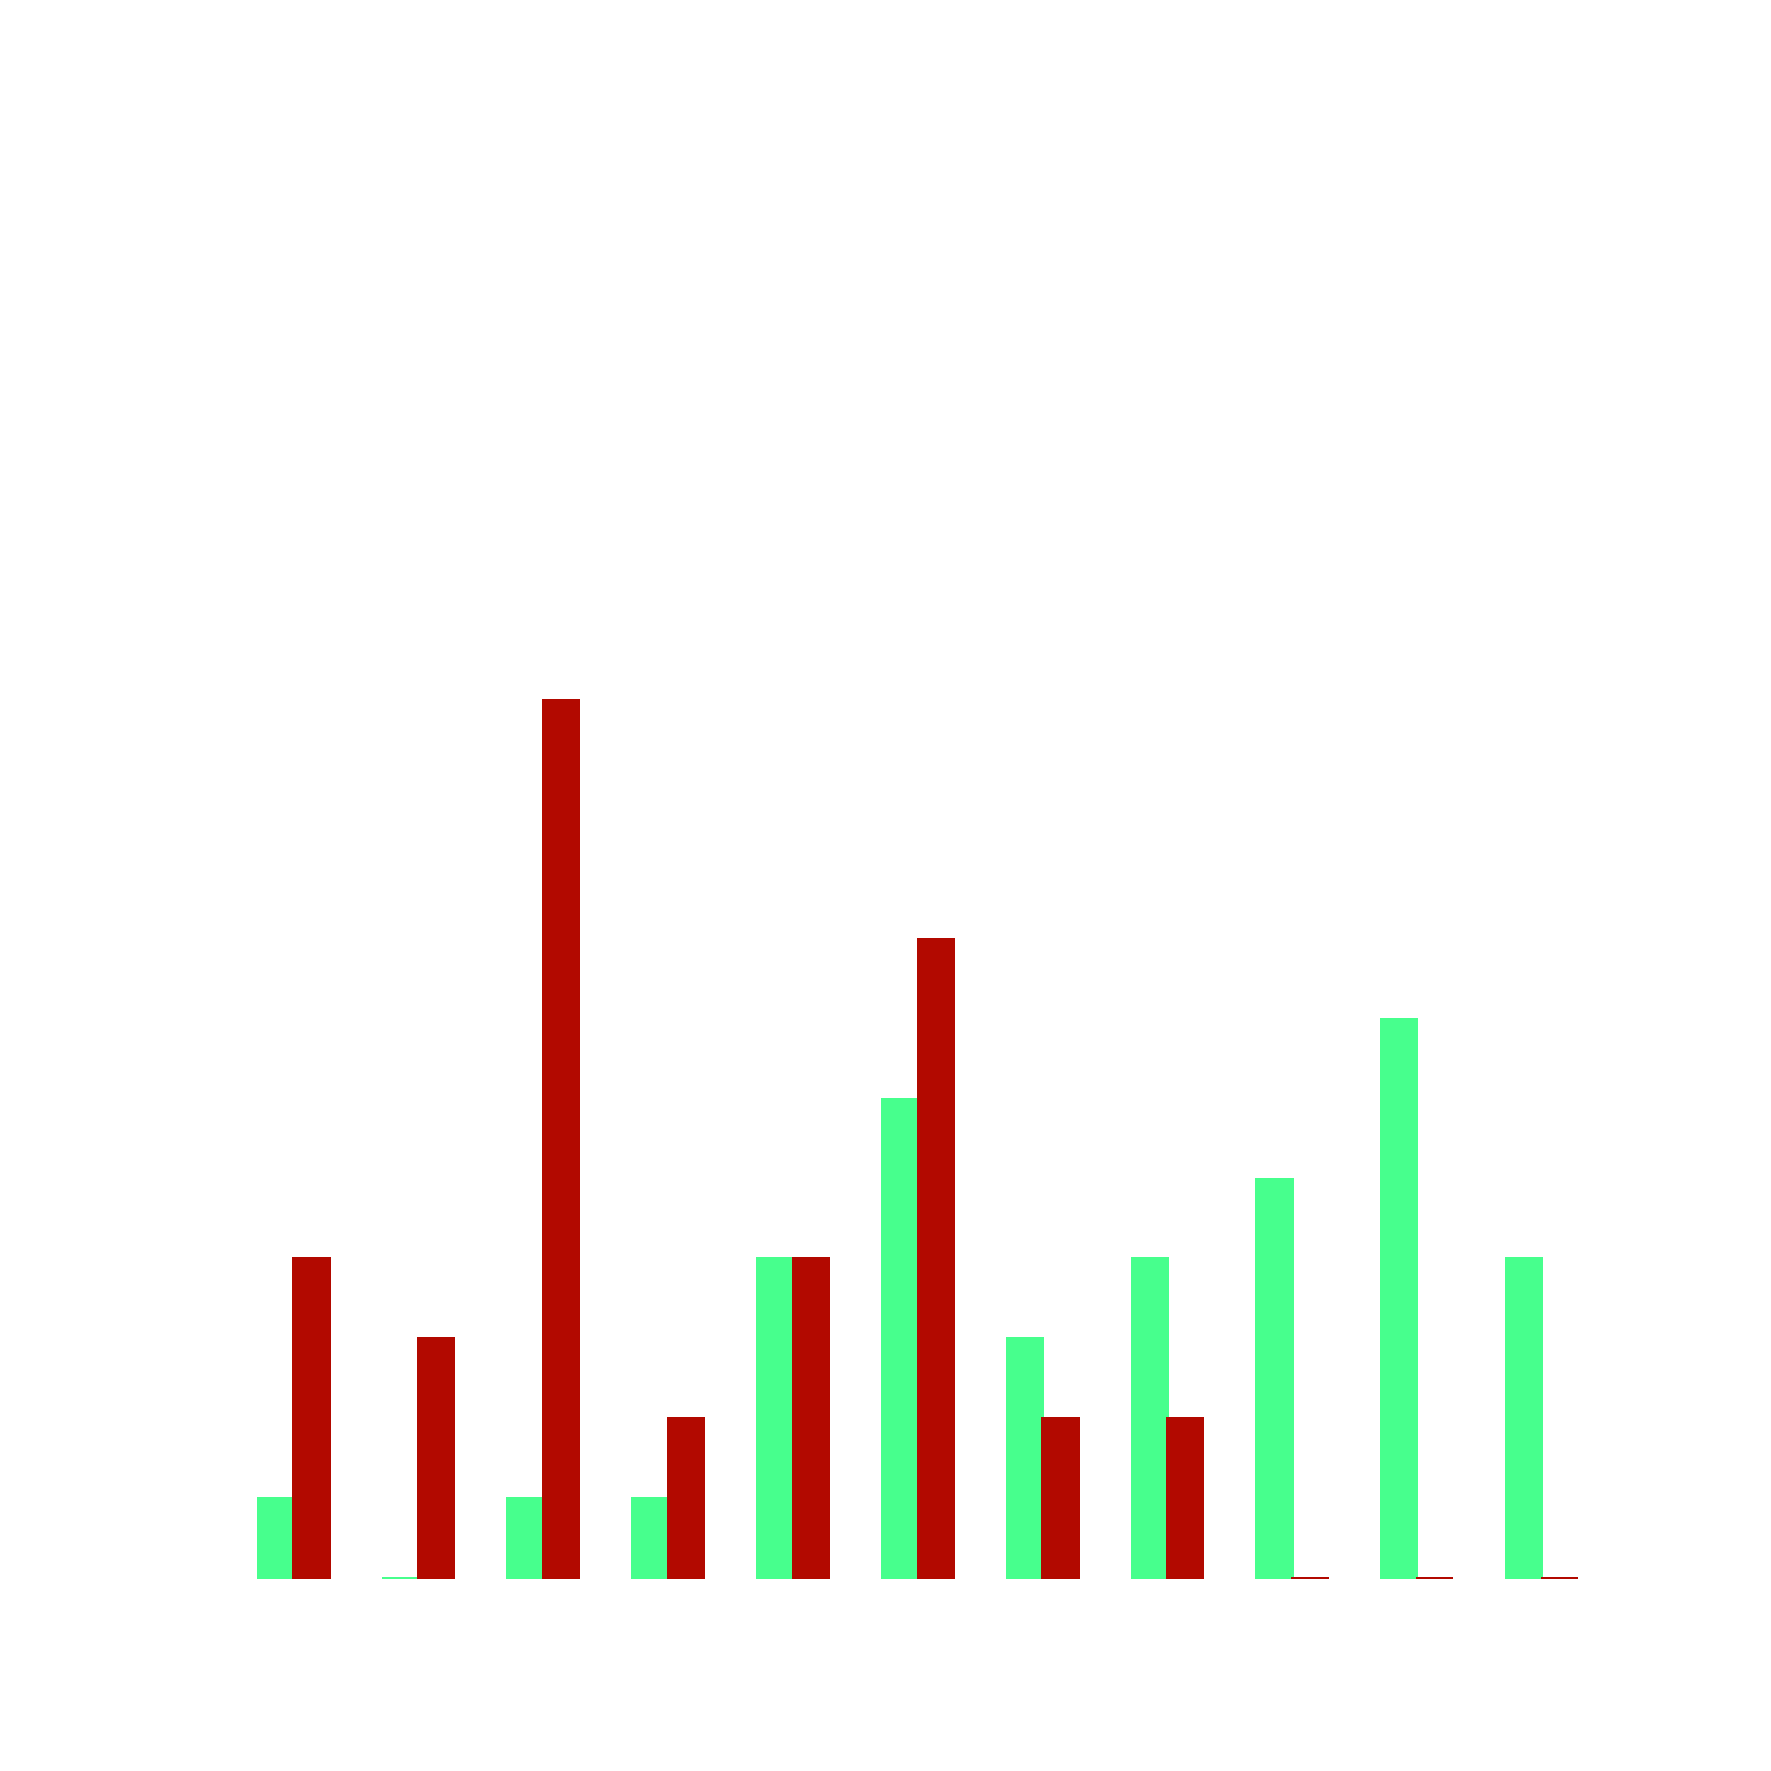
\includegraphics[width=.16\linewidth]{gfxXpUrbanSoundscape/xp4_note_1}\label{fig:xp4_note_1a}}
        \subfloat[sujet 2]
        {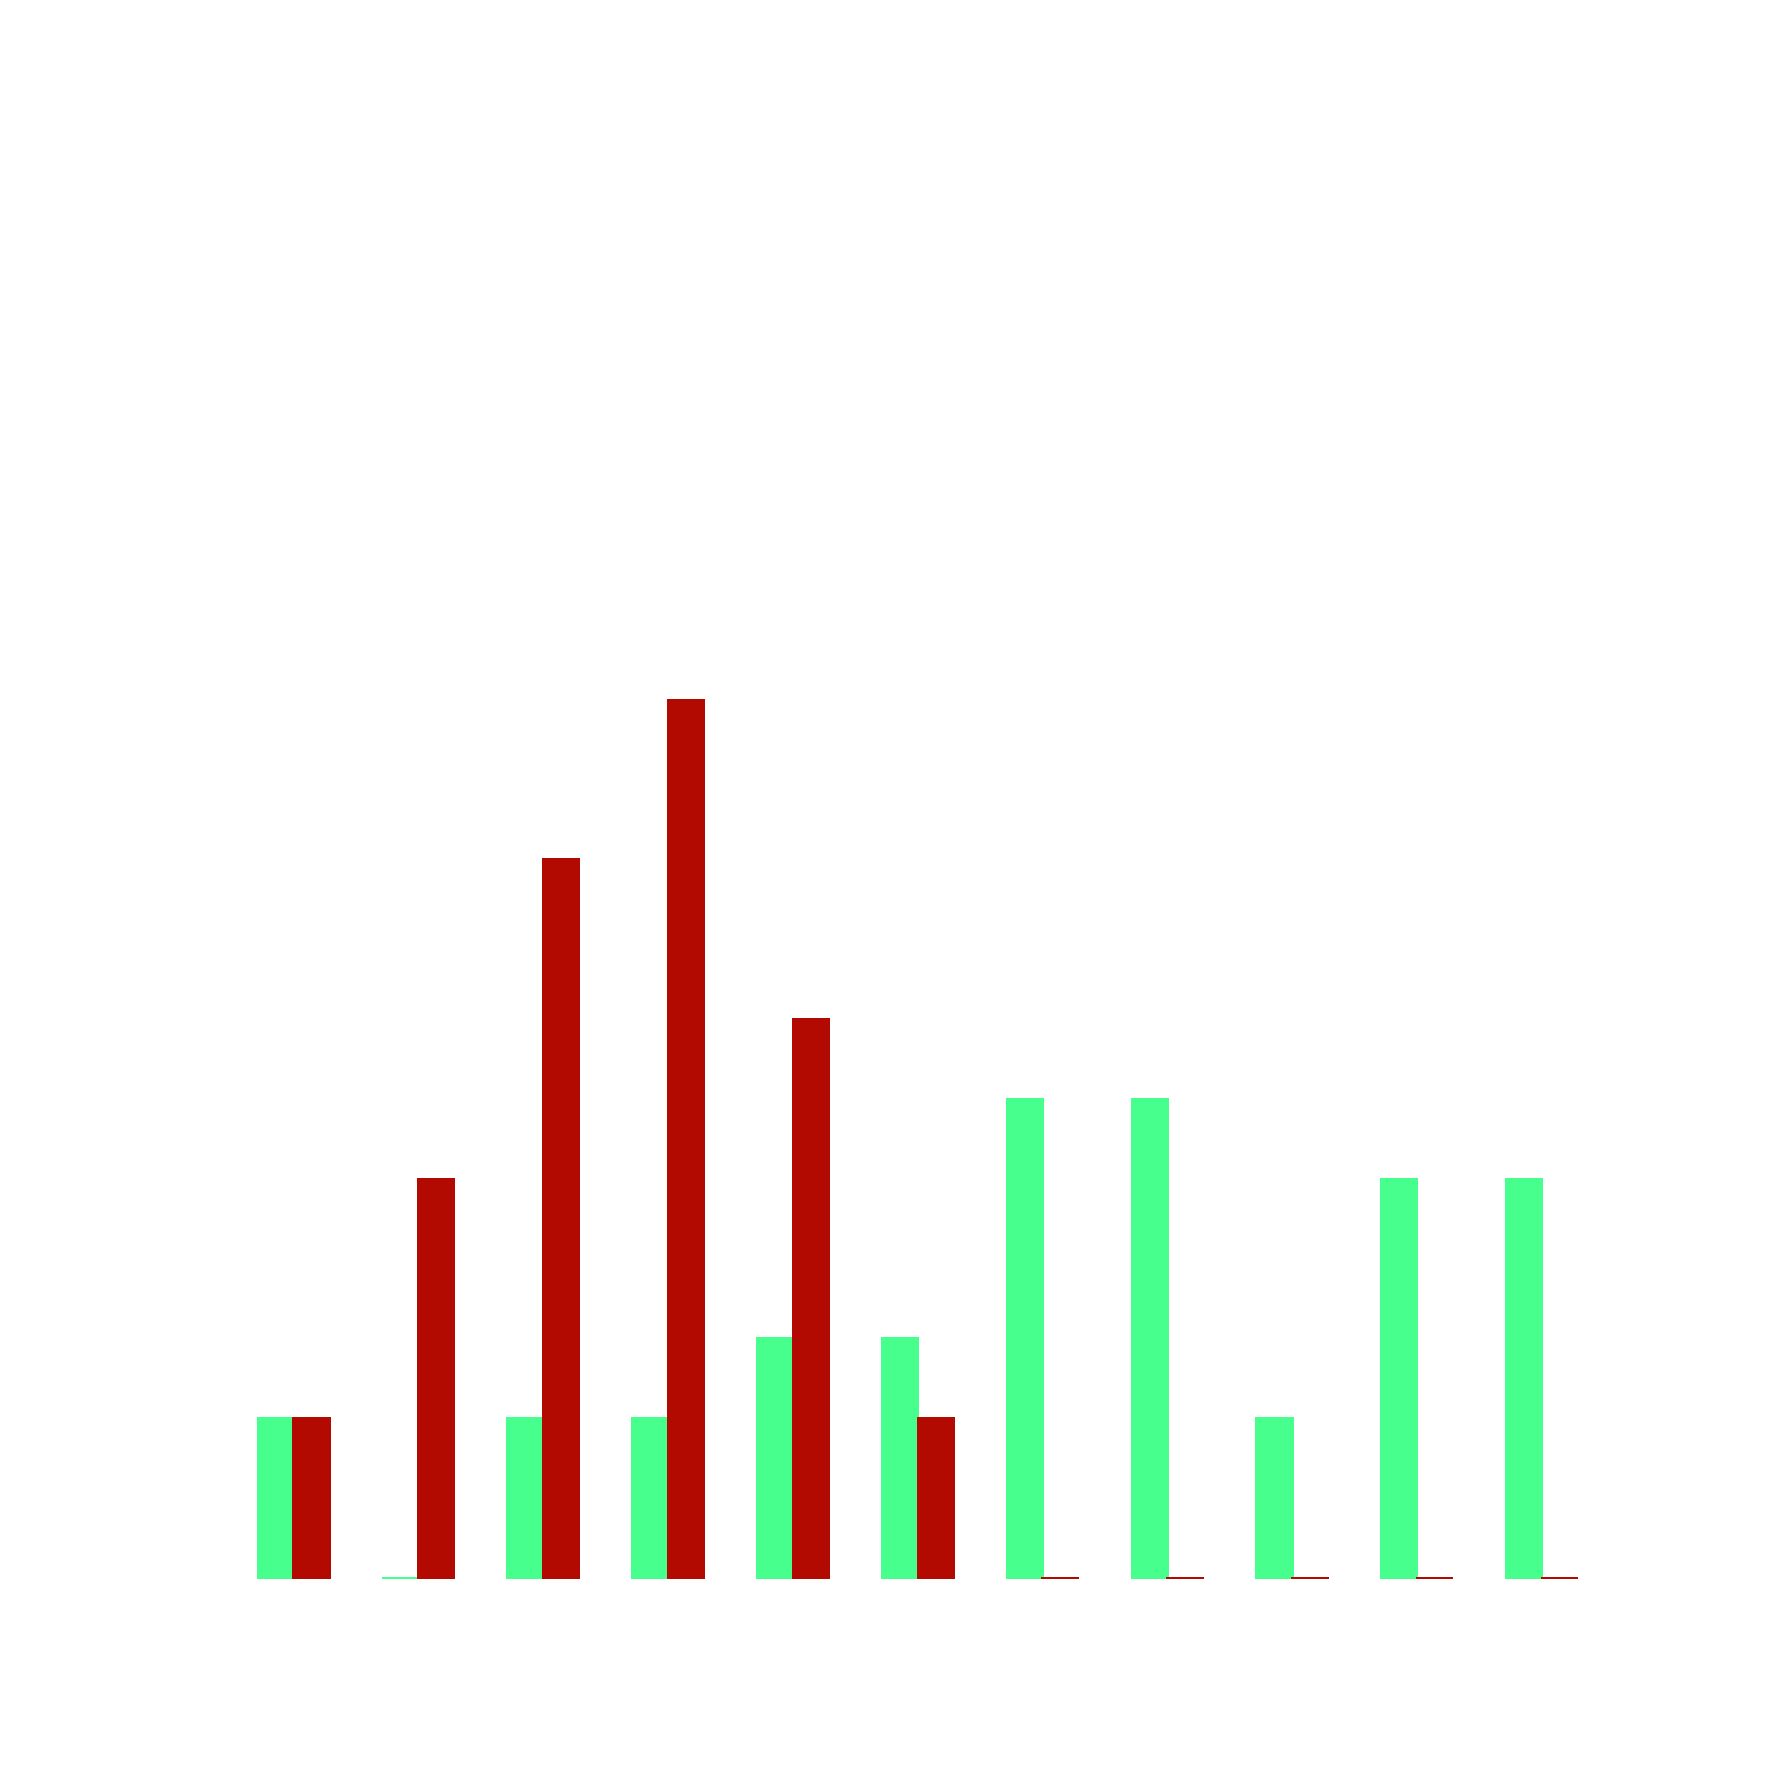
\includegraphics[width=.16\linewidth]{gfxXpUrbanSoundscape/xp4_note_2}\label{fig:xp4_note_1b}}
        \subfloat[sujet 3]
        {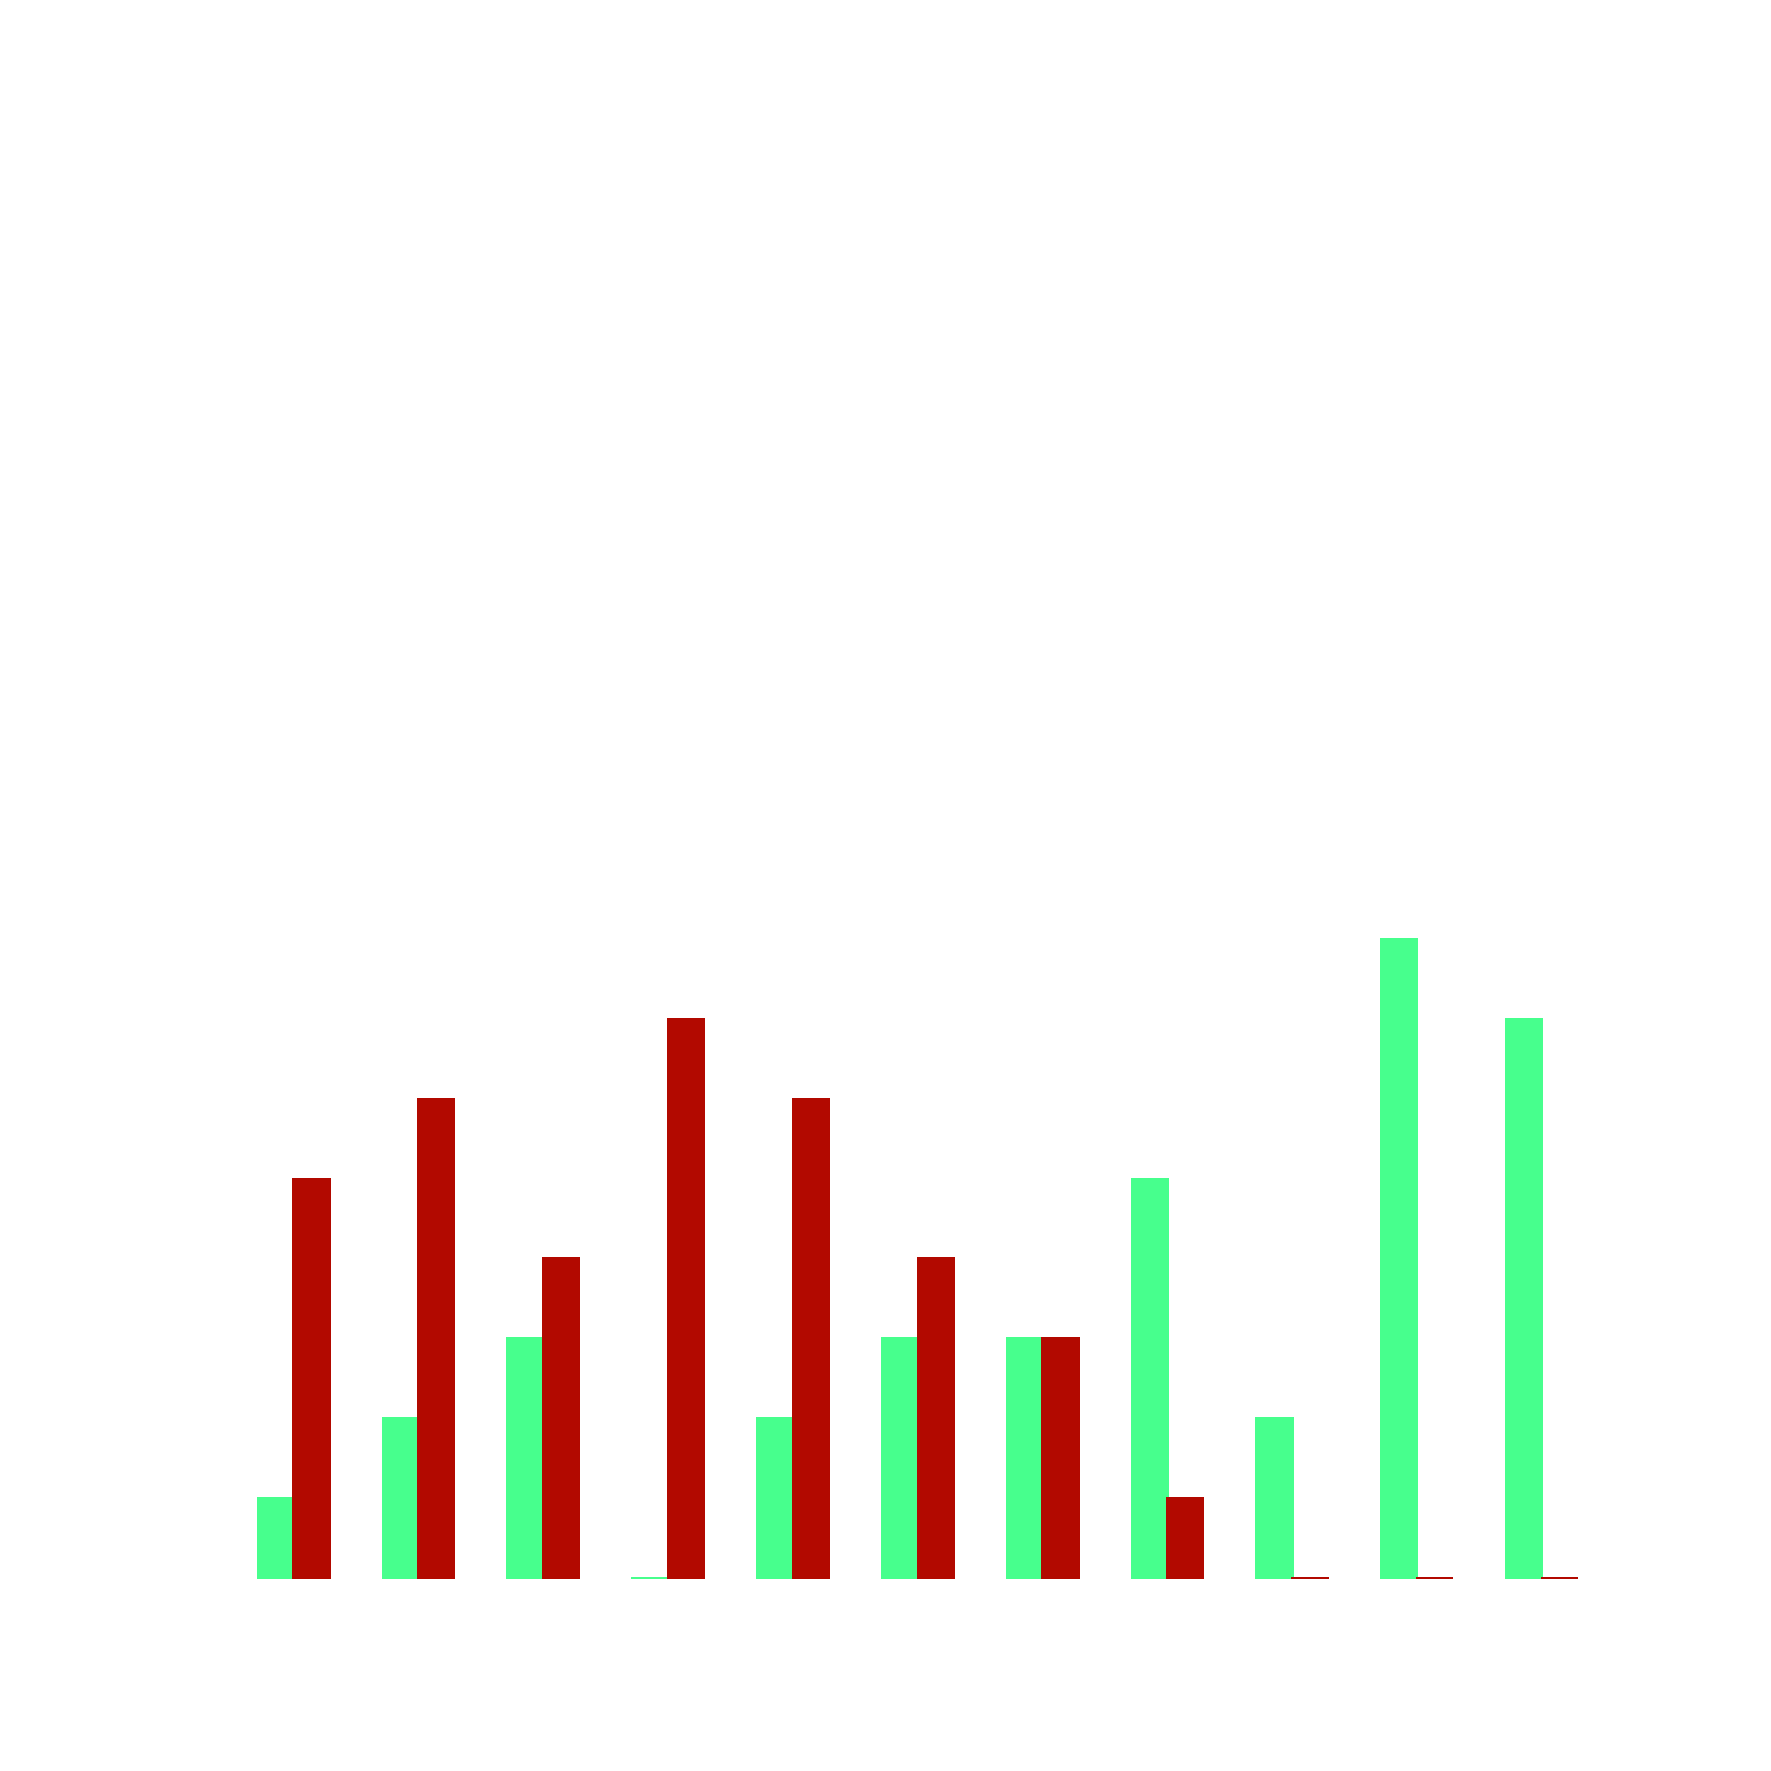
\includegraphics[width=.16\linewidth]{gfxXpUrbanSoundscape/xp4_note_3}\label{fig:xp4_note_1c}}
        \subfloat[sujet 4]
        {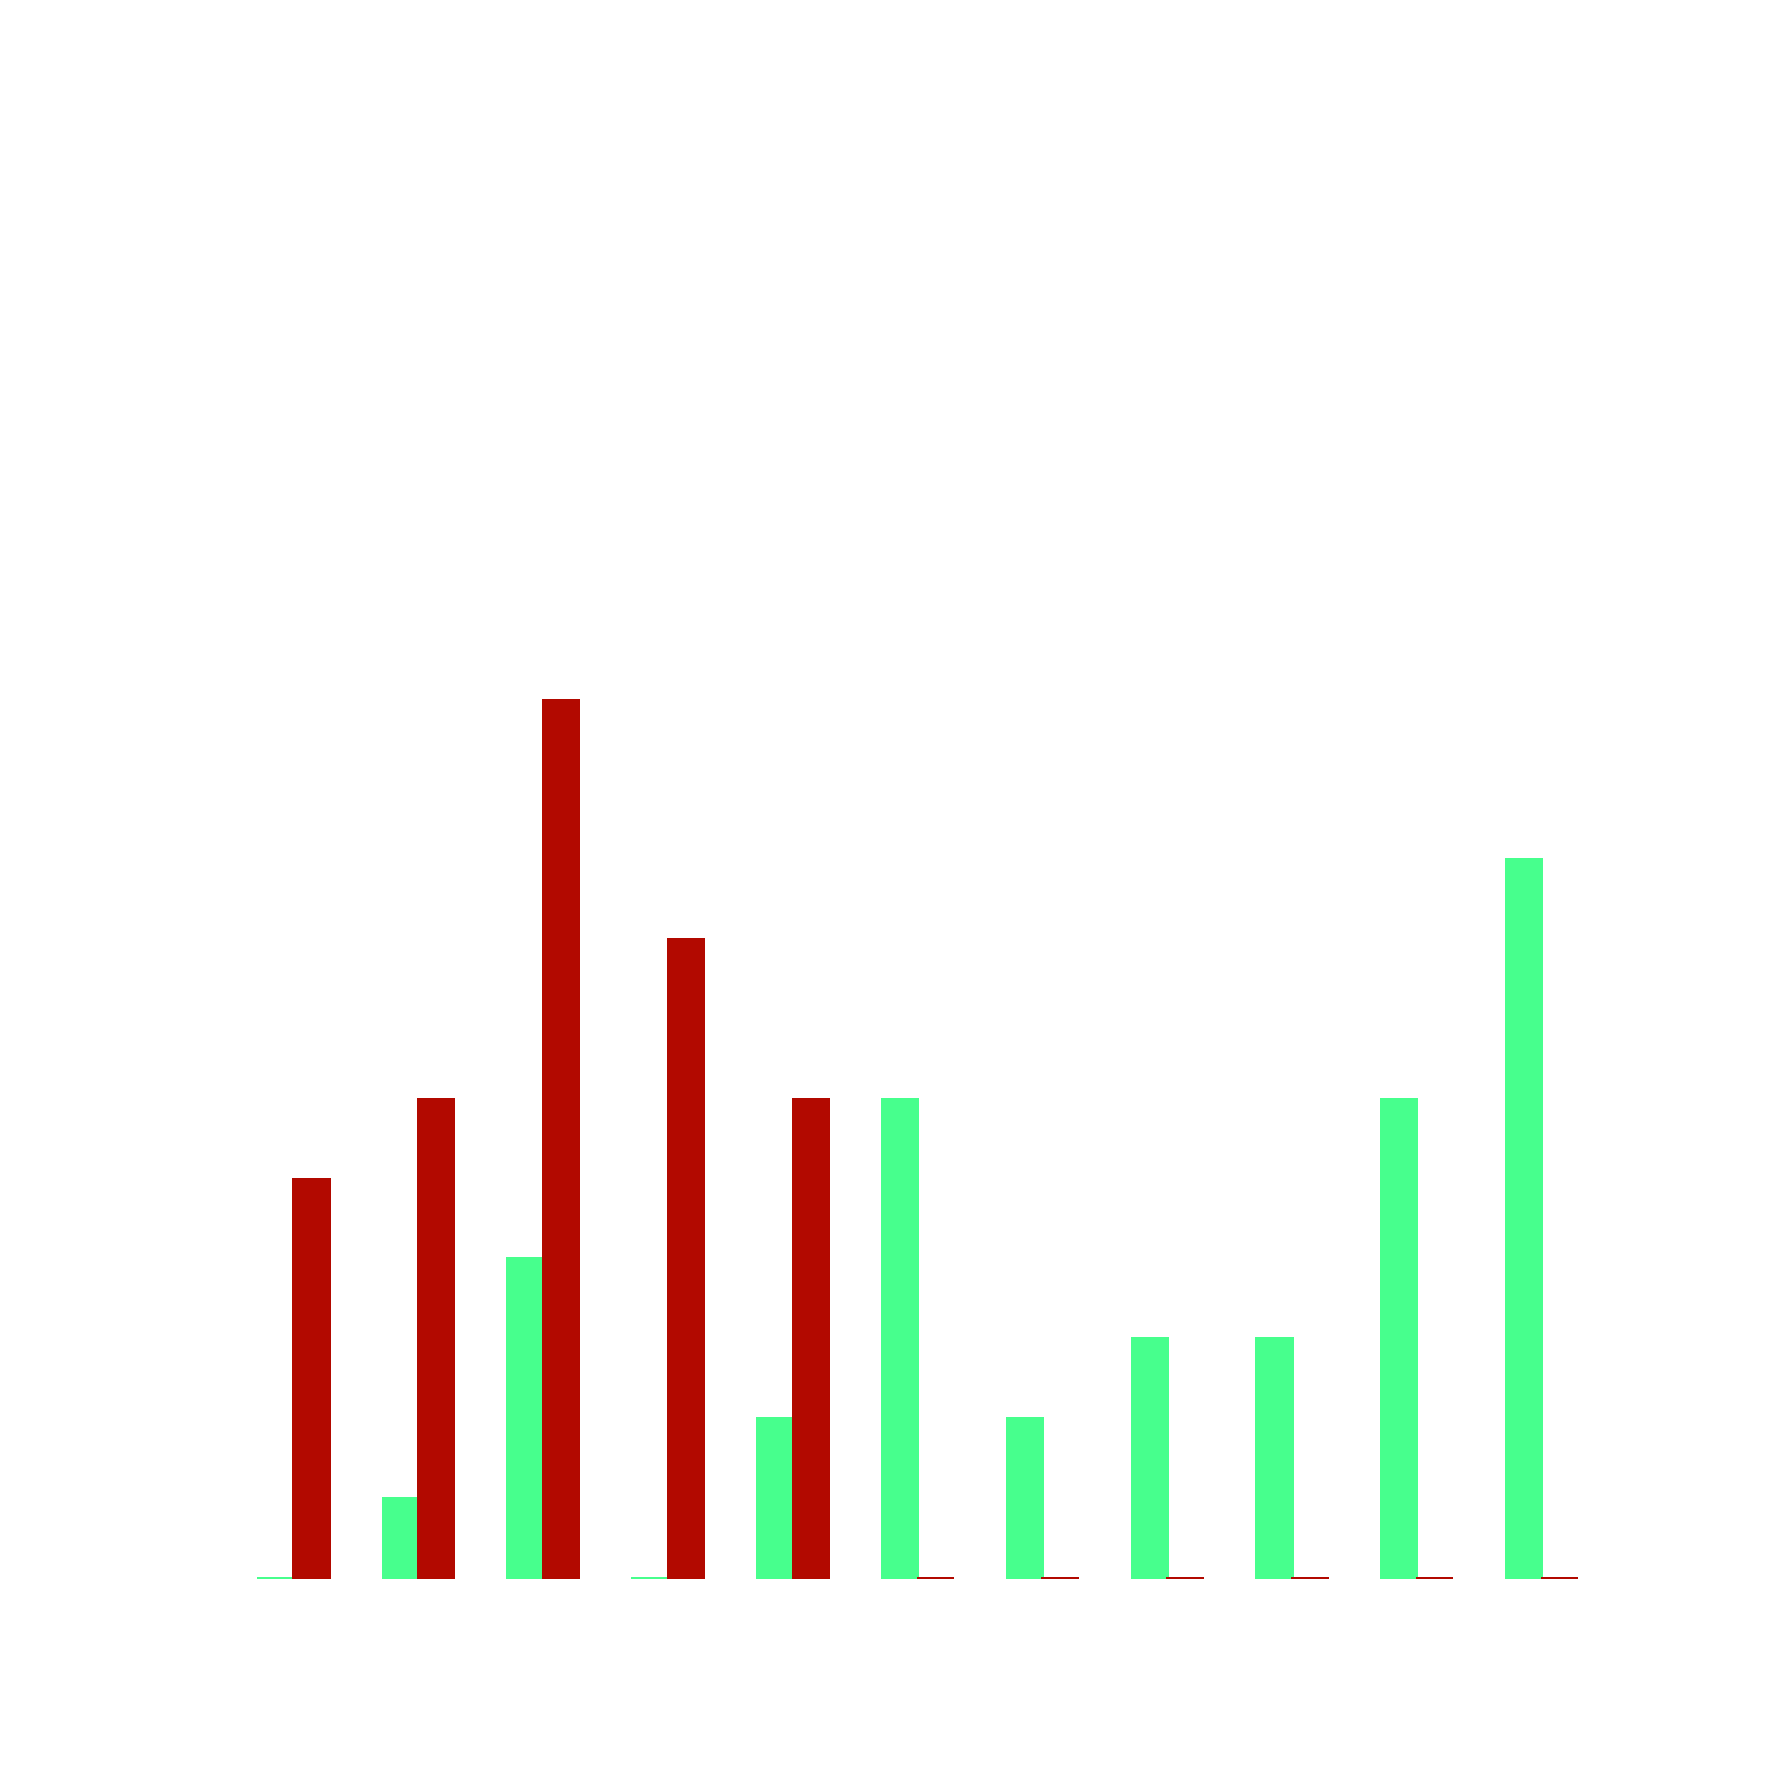
\includegraphics[width=.16\linewidth]{gfxXpUrbanSoundscape/xp4_note_4}\label{fig:xp4_note_1d}}
        \subfloat[sujet 5]
        {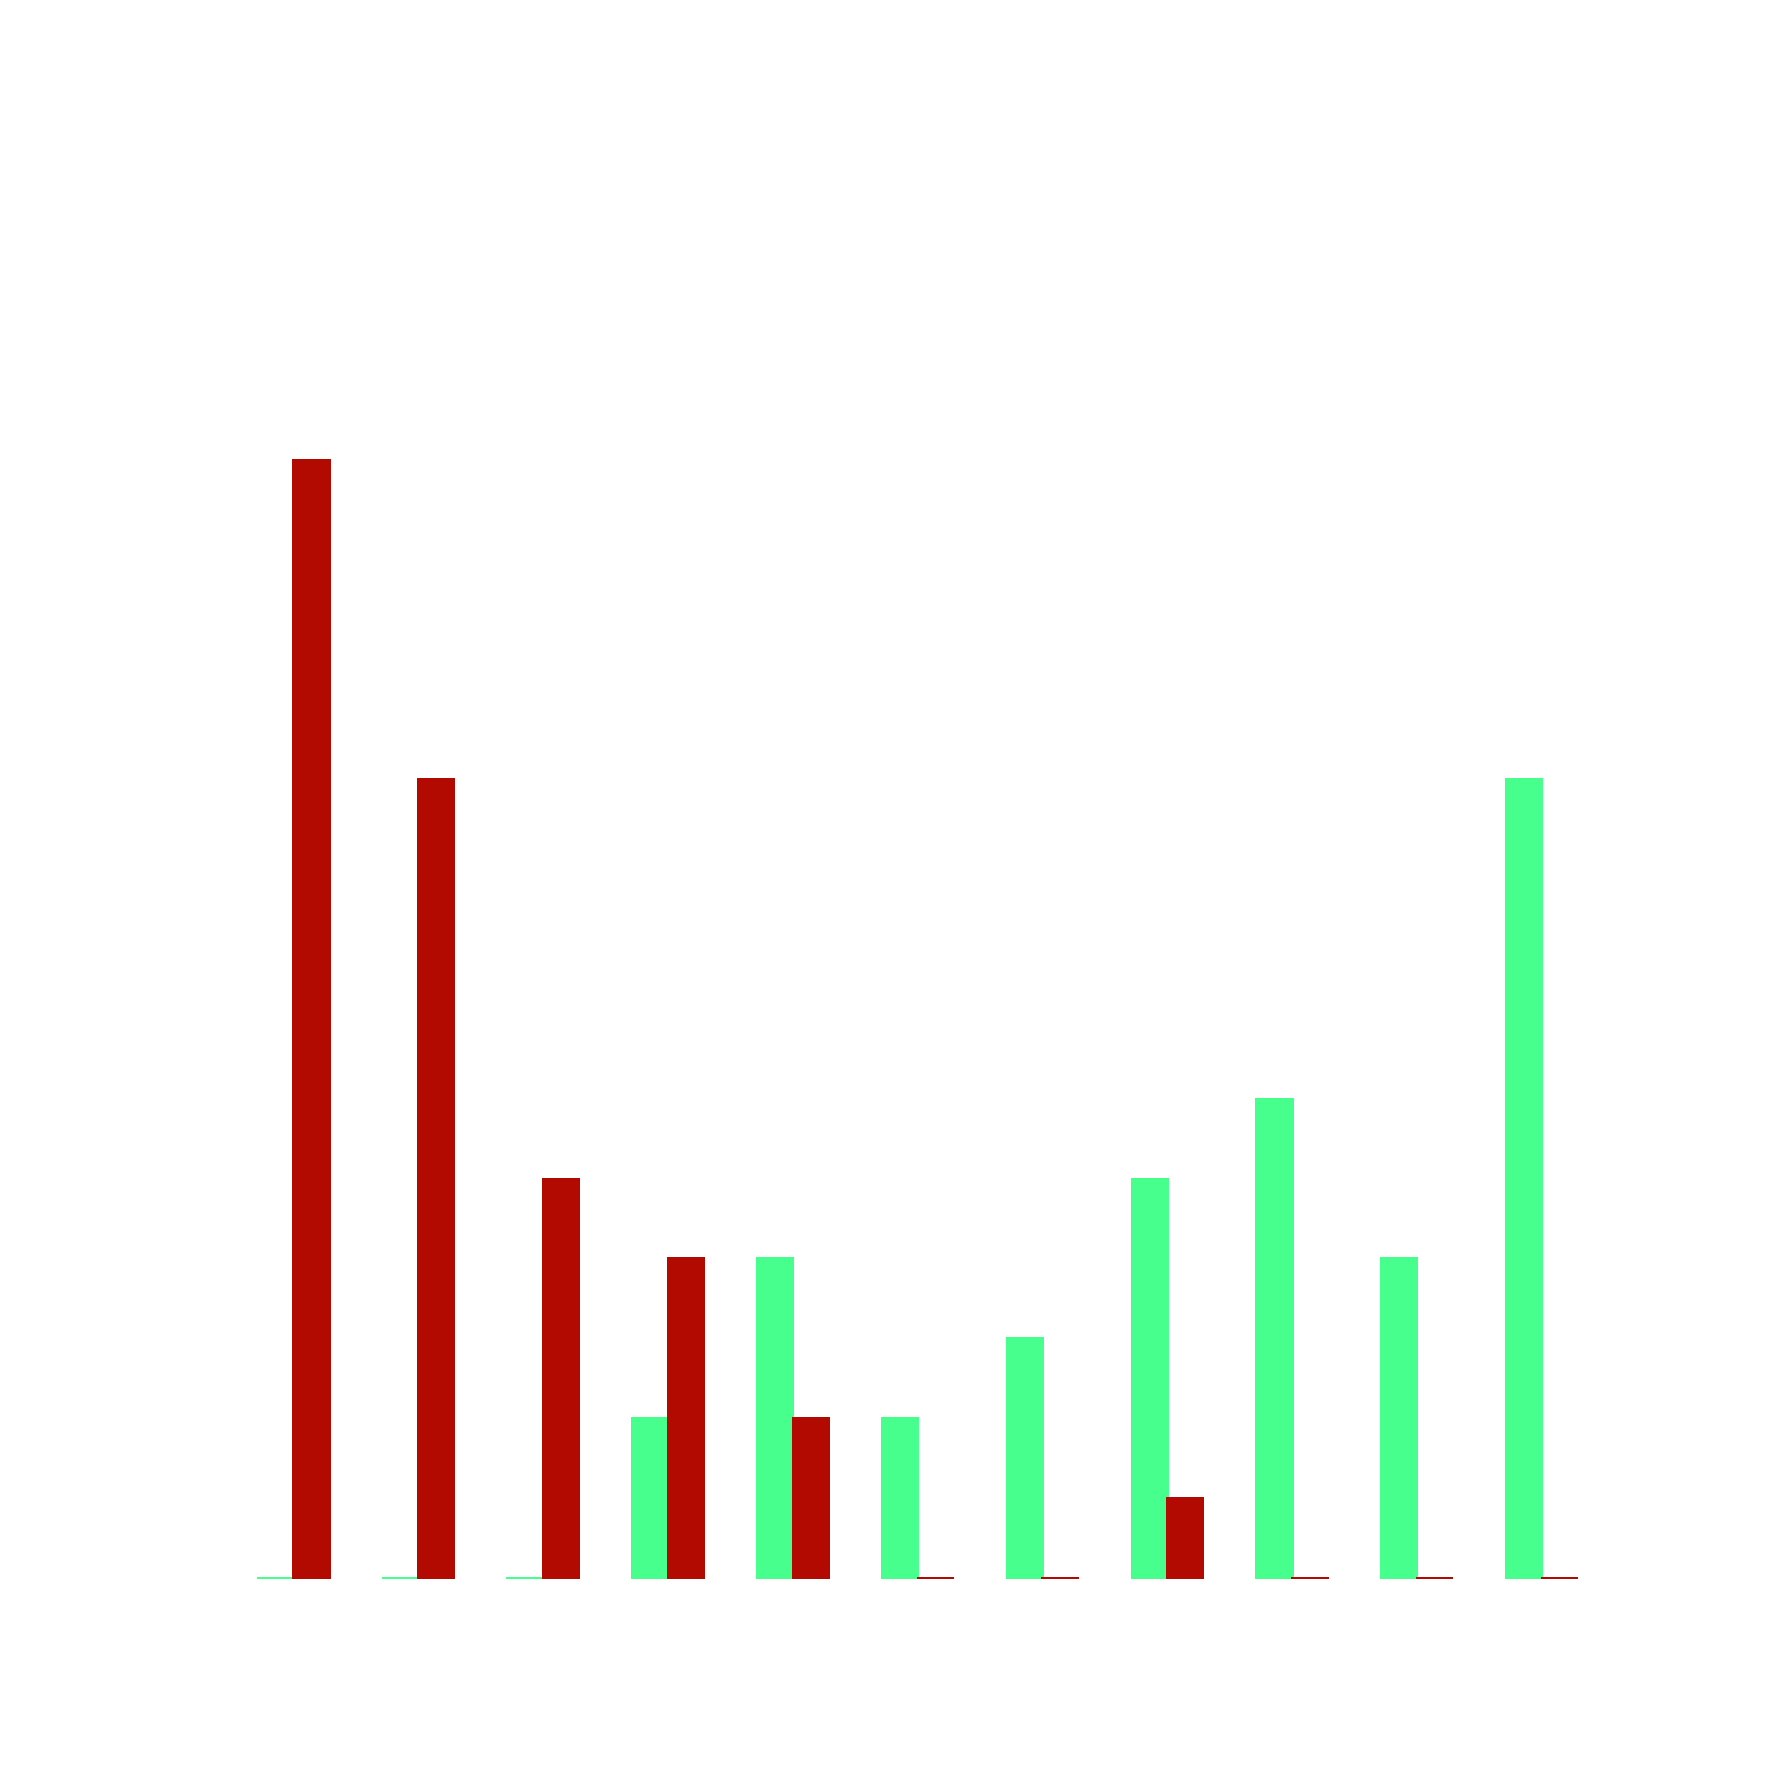
\includegraphics[width=.16\linewidth]{gfxXpUrbanSoundscape/xp4_note_5}\label{fig:xp4_note_1e}}
        \subfloat[sujet 6]
        {\includegraphics[width=.16\linewidth]{gfxXpUrbanSoundscape/xp4_note_6}\label{fig:xp4_note_1f}}\par       
        \subfloat[sujet 7]
        {\includegraphics[width=.16\linewidth]{gfxXpUrbanSoundscape/xp4_note_7}\label{fig:xp4_note_1g}}
        \subfloat[sujet 8]
        {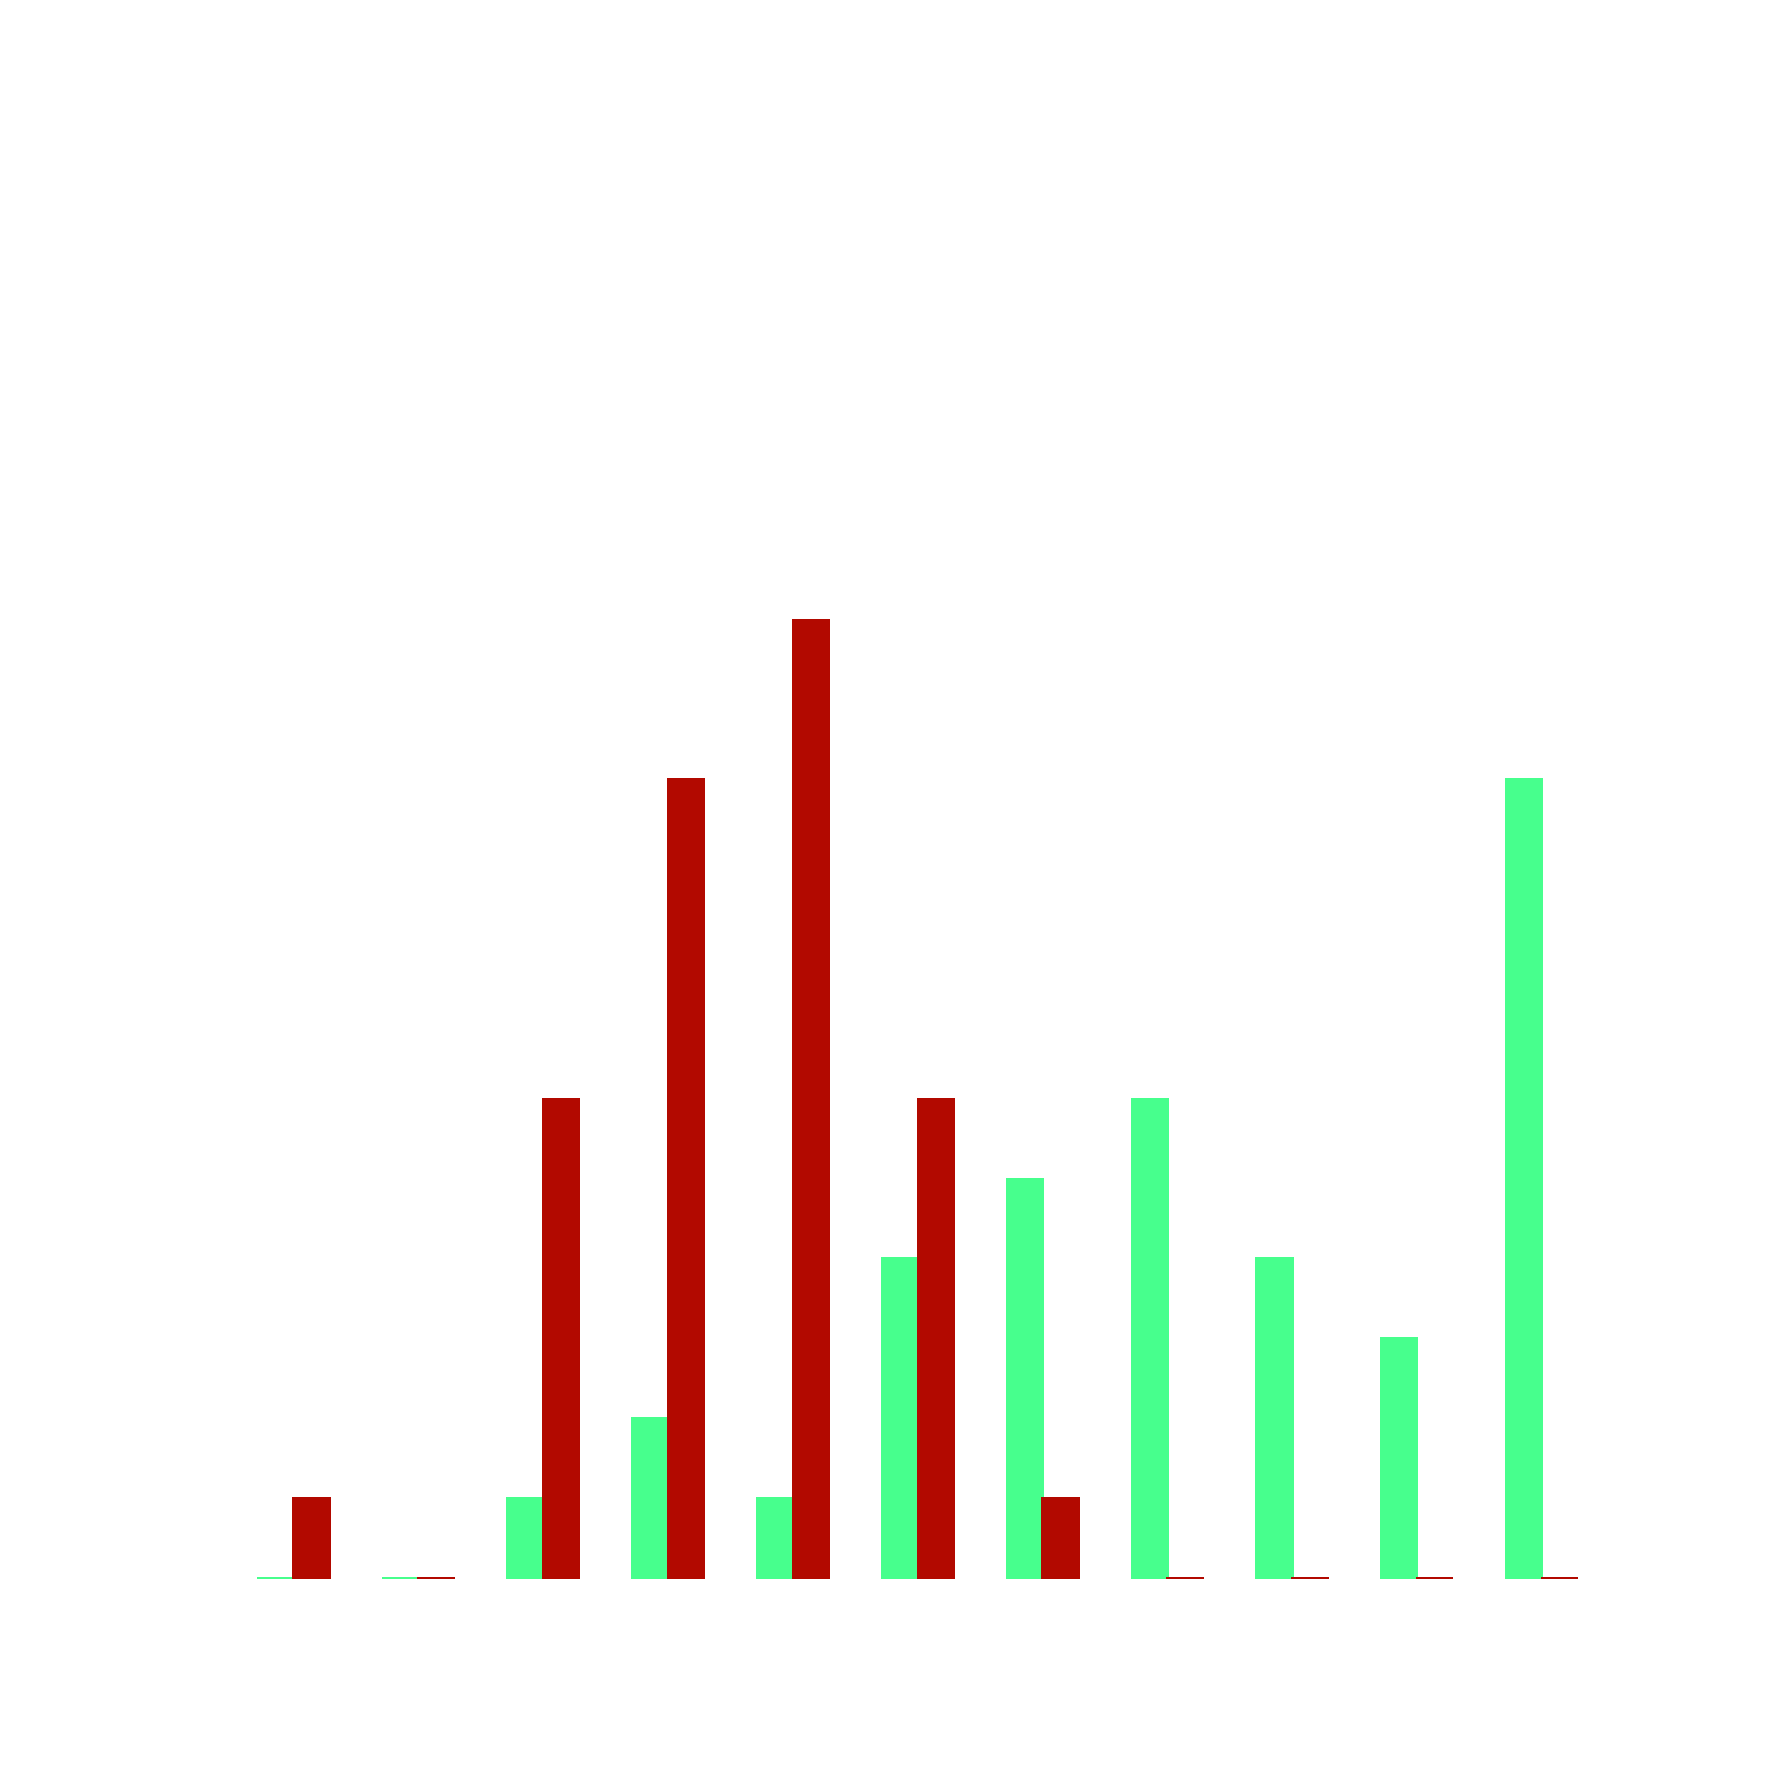
\includegraphics[width=.16\linewidth]{gfxXpUrbanSoundscape/xp4_note_8}\label{fig:xp4_note_1h}}
        \subfloat[sujet 9]
        {\includegraphics[width=.16\linewidth]{gfxXpUrbanSoundscape/xp4_note_9}\label{fig:xp4_note_1i}}
        \subfloat[sujet 10]
        {\includegraphics[width=.16\linewidth]{gfxXpUrbanSoundscape/xp4_note_10}\label{fig:xp4_note_1j}}
        \subfloat[sujet 11]
        {\includegraphics[width=.16\linewidth]{gfxXpUrbanSoundscape/xp4_note_11}\label{fig:xp4_note_1h}}
        \subfloat[sujet 12]
        {\includegraphics[width=.16\linewidth]{gfxXpUrbanSoundscape/xp4_note_12}\label{fig:xp4_note_1l}}       
        \caption[TODO]{TODO}\label{fig:xp4_note_1}
\end{figure}


\begin{figure}[t]
        \myfloatalign
        \subfloat[]
        {\includegraphics[width=.33\linewidth]{gfxXpUrbanSoundscape/xp4_note_13}\label{fig:xp4_note_2}}
        \subfloat[]
        {\includegraphics[width=.33\linewidth]{gfxXpUrbanSoundscape/xp4_note_15}\label{fig:xp4_note_4}}
        \subfloat[]
        {\includegraphics[width=.33\linewidth]{gfxXpUrbanSoundscape/xp4_note_16}\label{fig:xp4_note_5}}
       \caption[TODO]{TODO}\label{fig:xp4_note_245}
\end{figure}


\subsection{Influence des descripteurs structurels des scènes avec marqueurs sur l'agrément perçu: une analyse comparative}

Cette section présente une étude comparative entre les résultats de l'expérience 1.b, et ceux obtenus, pour les am-scènes,dans l'expérience ci-après. 

Nous commençons par évaluer la corrélation entre les $\mathcal{A}_{scene}$ obtenues par les deux études. Les résultats sont affichés sur la figure~\ref{fig:xp4_note_5}. La corrélation est élevée, que l'on considère l'ensemble des scènes ($r=0.98$, $p<0.01$), ou les i- ($r=0.82$, $p<0.01$), ou encore les ni-scènes  ($r=0.91$, $p<0.01$).

Concernant les différences de $\mathcal{A}_{sujet}$ entre les i/am- et ni/am-scenes, nous observons un delta net et significatif ($p<0.01$), avec une différence moyenne des écarts de 4.5. Ces résultats sont en accord avec ceux de l'expérience 1.b.

Comme pour l'expérience 1.b, une analyse des relations entre les descripteurs structurels et $\mathcal{A}_{scene}$ est réalisée. Les résultats sont affichés dans le tableau~\ref{tab:corrAmXP4}. Ce tableau fait apparaître des différences: 

Considérons les niveaux ($L$, $L(E)$ et $L(T)$) pour les i-scènes. Une corrélation modérée négative est observée entre ces descripteurs et $\mathcal{A}_{scene}$, alors qu'aucune n'était observée pour l'expérience 1.b. Il apparaît, dans l'expérience 2, que ces descripteurs ont joué un rôle (négatif) plus important dans l'évaluation des qualités affectives des scènes, que dans l'expérience 1.b. Cependant, l'observation précédemment faite, sur le fait que ces descripteurs n'impactent pas de la même manière la perception des i et ni-scènes, se maintient. En effet les corrélations pour les niveaux restent modérées pour les i-scènes ($r<-0.46$), alors que celles observées pour les ni-scènes sont toutes élevées ($r>-0.81$). Le niveau est donc bien pris en compte dans l'évaluation des i-scènes, mais moins que dans l'évaluation des ni-scènes. Cette recrudescence de l'importance du niveau est également observée sur $L_b$ pour les ni-scènes ($r=-0.40$, $p<0.05$), ainsi que sur $L(T)_b$ ($r=-0.46$, $p<0.01$) pour les i-scènes, mais là encore les corrélations reste modérées voire faibles.

Deux différences concernant les densités sont relevées. Nous observons une corrélation modérée sur $D$ pour les i-scènes ($r=-0.42$, $p<0.05$) et une corrélation faible pour $D(E)$ ($r=-0.42$, $p<0.05$). Comme pour le niveau, la densité semble avoir une influence plus importante dans l'expérience 2. 

La majorité des différences concerne les descripteurs des i-scènes. Pour tous ces descripteurs, les corrélations observées pour les ni-scènes sont plus importantes pour l'expérience 2 que pour l'expérience 1.b. Considérant les différences d'appréciation entre les i- et ni-scènes, les résultats restent donc consistant. Il apparaît que les descripteurs structurels de niveaux et de densités ont globalement plus influé sur l'agrément perçu dans l'expérience 2 que dans l'expérience 1.b.

Excepté ces points, tous les résultats observés dans les deux études concordent, notamment:

\begin{itemize}
\item l'effet bénéfique de l'émergence des i-marqueurs d'événements pour les i-scènes ($L_m-L_b$: $r=0.60$, $p<0.01$; $L(E)_m-L(E)_b$: $r=0.56$, $p<0.01$);
\item l'effet négatif des ni-marqueurs d'événements pour les ni-scènes ($L_m$: $r=0.75$, $p<0.01$; $L(E)_m$: $r=0.73$, $p<0.01$);
\item l'impact nul des marqueurs de textures pour les i- ($L(T)_m$: $r=-0.05$, $p=0.86$) et ni-scènes ($L(T)_m$: $r=-0.06$, $p=0.76$).
\end{itemize}


\gl{TODO: compléter}

\begin{table}[t]
\centering
\begin{tabular}{l r r} 
                   &   i-scènes                      & ni-scènes \\
\hline
$L$                & \textbf{-0.46$^{*}$} ($p<0.01$) & \textbf{-0.83} ($p<0.01$)\\
$L(E)$             & -0.33 ($p=0.05$)                & \textbf{-0.84} ($p<0.01$)\\
$L(T)$             & \textbf{-0.42$^{*}$} ($p<0.05$) &  0.04 ($p=0.81$) \\
$D$                & \textbf{-0.42$^{*}$} ($p<0.05$) & \textbf{-0.47} ($p<0.01$)\\
$D(E)$             & \textbf{-0.36$^{*}$} ($p<0.05$) & \textbf{-0.57} ($p<0.01$)\\
$DIV(E)$ 0         & -0.26 ($p=0.13$)                & -0.32 ($p=0.06$)\\
$DIV(E)$ 1         & -0.29 ($p=0.10$)                & -0.31 ($p=0.06$)\\
$DIV(E)$ 2         & -0.24 ($p=0.17$)                & -0.32 ($p=0.06$)\\
$DIV(E)$ 3         & -0.20 ($p=0.25$)                & -0.31 ($p=0.06$)\\
$L_m$              & 0.16  ($p=0.36$)                & \textbf{-0.75} ($p<0.01$) \\
$L(E)_m$           & 0.08  ($p=0.64$)                & \textbf{-0.73} ($p<0.01$) \\
$L(T)_m$           & -0.05 ($p=0.86$)                & -0.06 ($p=0.76$) \\
$L_b$              & \textbf{-0.64} ($p<0.01$)       & \textbf{-0.40$^{*}$} ($p<0.05$) \\
$L(E)_b$           & \textbf{-0.57} ($p<0.01$)       & -0.33 ($p=0.05$) \\
$L(T)_b$           & \textbf{-0.46$^{*}$} ($p<0.01$) & \textbf{-0.83} ($p<0.01$) \\
$L_m-L_b$          & \textbf{0.60} ($p<0.01$)        & -0.25 ($p=0.14$) \\
$L(E)_m-L(E)_b$    & \textbf{0.56} ($p<0.01$)        & -0.27 ($p=0.11$) \\
$L(T)_m-L(T)_b$    & 0.43 ($p=0.07$)                 & 0.36 ($p=0.05$) \\
$D_m$              & -0.12 ($p=0.48$)                & -0.33 ($p=0.05$) \\
$D(E)_m$           & -0.21 ($p=0.22$)                & \textbf{-0.53} ($p<0.01$) \\
\hline
\end{tabular}
\vspace{0.5mm}
\caption{\gl{TODO: i/am-scenes et ni/am-scenes}}
\label{tab:corrAmXP4}
\end{table}

\subsection{Influence de la présence des marqueurs sur l'agrément perçu}
\label{sec:ch5_Asujet}

Dans cette section nous étudions comment les sujets ont perçu les différents types de scènes, nommément: i/am-, ni/am-, i/sm- et ni/sm-scène. L'ANOVA à mesures répétées pratiquée sur $\mathcal{A}_{sujet}$ (\cf~Figure~\ref{fig:xp4_note_2}) montre un effet significatif du type d'environnements (i/ni: $F[1,10]=175$, $p<0.01$), de la présence/absence des marqueurs (am/sm: $F[1,10]=7$, $p<0.05$) , ainsi que de l'interaction entre les deux facteurs ($F[1,10]=67$, $p<0.01$).

L'analyse \emph{post hoc} montre, quant à elle, des différences significatives entre tous les groupes d'observations, notamment entre les i/am- et i/sm-scenes ($p<0.05$) et les ni/am- et ni/sm-scenes ($p<0.01$).


Ces résultats indiquent que la suppression des événements a effectivement modifié la perception des scènes par les sujets. Nos deux hypothèses sont ainsi vérifiées:

\begin{itemize}
\item la suppression des ni-marqueurs a amélioré les qualités perçues des ni-scènes;
\item la suppression des i-marqueurs a diminué les qualités perçues des i-scènes.
\end{itemize}

L'interaction significative montre que l'effet du type d'environnements influe sur l'effet dû à l'absence/présence des marqueurs. En effet la moyenne des écarts entre les am- et sm-scènes est plus importante pour les ni-scènes (1.1) que pour les i-scènes (0.5). 

Les i-marqueurs ont donc bien un effet bénéfique sur la perception d'un environnement. Le fait que leur suppression diminue $\mathcal{A}_{scene}$ montre clairement qu'il est possible d'améliorer la qualité d'un environnement en ajoutant des sons bien acceptés comme \emph{oiseaux}. Ces conclusions vont dans le sens de l'approche positive comme introduite par Schafer \citep{schafer1977tuning} (\cf~Section~\ref{sec:ch3_urbanNoiseSoundscape}). \\

\gl{TODO: citation}

\subsection{Influence des descripteurs structurels des scènes sans marqueurs sur l'agrément perçu}

L'ANOVA mixte pratiquée sur $\mathcal{A}_{scene}$ (\cf~Figure~\ref{fig:xp4_note_4}) montre un effet significatif du type d'environnements (i/ni: $F[1,70]=222$, $p<0.01$), de la présence/absence des marqueurs (am/sm: $F[1,70]=5$, $p<0.05$) , ainsi que de l'interaction entre les deux facteurs ($F[1,70]=35$, $p<0.01$).

L'analyse \emph{post hoc} montre des différences significatives entre tous les groupes d'observations, notamment, là encore, entre les i/am- et i/sm-scenes ($p<0.05$) et les ni/am- et ni/sm-scenes ($p<0.01$).

Ainsi, les quatre types de scènes, considérant $\mathcal{A}_{scene}$ comme indicateur, forment bien quatre groupes distincts. L'interaction montre que le type d'environnement impacte l'effet provoqué par la suppression des marqueurs, les moyennes d'écart étant identiques à celles de l'analyse de la section précédente (ni-scènes: 1.1,  i-scènes: 0.5, \cf~Section~\ref{sec:ch5_Asujet}).
 
\begin{table}[t]
\centering
\begin{tabular}{l c c c} 
               & ensemble                     & i-scènes                   & ni-scènes    \\
\hline
$L$            & \textbf{-0.79} ($p<0.01$)    & \textbf{-0.49} ($p<0.01$)  & \textbf{-0.74} ($p<0.01$)\\
$L(E)$         & \textbf{-0.76} ($p<0.01$)    & \textbf{-0.44} ($p<0.01$)  & \textbf{-0.70} ($p<0.01$)\\
$L(T)$         & \textbf{-0.41} ($p<0.01$)    & -0.17 ($p=0.36$)           & -0.44 ($p=0.80$) \\
$D$            & \textbf{-0.49} ($p<0.01$)    & -0.31 ($p=0.07$)           & -0.29 ($p=0.08$)\\
$D(E)$         & \textbf{-0.45} ($p<0.01$)    & -0.29 ($p=0.09$)           & \textbf{-0.39} ($p<0.05$)\\
$DIV(E)$ 0     &         -0.10  ($p=0.40$)    & -0.26 ($p=0.13$)           & -0.32 ($p=0.06$)\\
$DIV(E)$ 1     & \textbf{-0.49} ($p<0.01$)    & -0.29 ($p=0.09$)           & -0.31 ($p=0.06$)\\
$DIV(E)$ 2     & \textbf{-0.43} ($p<0.01$)    & -0.24 ($p=0.17$)           & -0.32 ($p=0.06$)\\
$DIV(E)$ 3     & \textbf{-0.39} ($p<0.01$)    & -0.20 ($p=0.25$)           & -0.32 ($p=0.06$)\\
\hline
\end{tabular}
\vspace{0.5mm}
\caption{\gl{TODO: i/sm-scenes et ni/sm-scenes}}
\label{tab:corrSmXP4}
\end{table}

\begin{figure}[t]
        \myfloatalign
        \includegraphics[width=.8\linewidth]{gfxXpUrbanSoundscape/xp4_div_1}
        \caption[TODO]{TODO}\label{fig:diversitySansMarker}
\end{figure}

\begin{figure}[t]
        \myfloatalign
        \subfloat[]
        {\includegraphics[width=.33\linewidth]{gfxXpUrbanSoundscape/xp4_density_13}\label{fig:densitySansMarkera}}
        \subfloat[]
        {\includegraphics[width=.33\linewidth]{gfxXpUrbanSoundscape/xp4_density_15}\label{fig:densitySansMarkerb}}\par
        \subfloat[]
        {\includegraphics[width=.33\linewidth]{gfxXpUrbanSoundscape/xp4_density_14}\label{fig:densitySansMarkerc}}
        \subfloat[]
        {\includegraphics[width=.33\linewidth]{gfxXpUrbanSoundscape/xp4_density_16}\label{fig:densitySansMarkerd}}
       \caption[TODO]{TODO}\label{fig:densitySansMarker}
\end{figure}

\begin{figure}[t]
        \myfloatalign
        \subfloat[]
        {\includegraphics[width=.33\linewidth]{gfxXpUrbanSoundscape/xp4_soundlevel_25}\label{fig:soundlevelSansMarkera}}
        \subfloat[]
        {\includegraphics[width=.33\linewidth]{gfxXpUrbanSoundscape/xp4_soundlevel_27}\label{fig:soundlevelSansMarkerb}}
        \subfloat[]
        {\includegraphics[width=.33\linewidth]{gfxXpUrbanSoundscape/xp4_soundlevel_29}\label{fig:soundlevelSansMarkerc}}\par
        \subfloat[]
        {\includegraphics[width=.33\linewidth]{gfxXpUrbanSoundscape/xp4_soundlevel_26}\label{fig:soundlevelSansMarkerd}}
        \subfloat[]
        {\includegraphics[width=.33\linewidth]{gfxXpUrbanSoundscape/xp4_soundlevel_28}\label{fig:soundlevelSansMarkere}}
        \subfloat[]
        {\includegraphics[width=.33\linewidth]{gfxXpUrbanSoundscape/xp4_soundlevel_30}\label{fig:soundlevelSansMarkerf}}       
        \caption[TODO]{TODO}\label{fig:soundlevelSansMarker}
\end{figure}

\subsection{Discussions}

\gl{TODO}

\section[Composition sémantique et catégorisation]{Influence de la composition sémantique sur les processus de catégorisation des scènes}
\label{sec:xp4}

\subsection{Objectif de l'expérience}

\subsection{Planification expérimentale}

\subsection{Données et méthodes d'analyses}

\subsection{Stratégie de catégorisation}

\begin{table}[t]
\centering
\begin{tabular}{lccccc}
subject & source  & location & quality & volume & frequency  \\
\hline
    $1^*$&        &          &    x    &        &           \\
    2    &   x    &          &         &        &           \\
    $3^*$&        &          &         &    x   &     x     \\
    4    &   x    &          &    x    &        &           \\
    5    &   x    &    x     &    x    &        &           \\        
    $6^*$&        &          &    x    &        &           \\
    7    &   x    &          &         &    x   &           \\
    $8^*$&        &          &    x    &        &           \\
    9    &   x    &    x     &         &        &           \\
    10   &   x    &          &         &        &           \\
\hline
\end{tabular}
\vspace{0.5mm}
\caption{\label{tab:StratSate} Strategies adopted by the subjects to categorize the scenes. Subjects removed from the data are indicated by $*$.}
\end{table}

\subsection{Du verbe à la classe}

\begin{table}[t]
\centering
\begin{tabular}{ccc}
labels                & categories         & classes\\
                      & (merging)          &        \\
\hline
alarm (2)             & alarm              &  \textit{car\_fire\_alarm} (sl-1) \\
                      & (alarm/siren/horn) &                                   \\
horn  (2)             & horn               &  \textit{horn} (sl-1)             \\
                      & (alarm/siren/horn) &                                    \\
siren (3)             & siren              &  \textit{siren} (sl-1)            \\
                      & (alarm/siren/horn) &                                    \\
birds (4)             & birds              &  \textit{birds} (sl-2)             \\
\hline
church bell (4)       & church bell        &  \textit{church bell} (sl-1)      \\
church (2)            &                    &                                   \\
\hline
mechanical            & construction       &  \textit{construction} (sl-0)       \\
public work  (4)      &                    &  \textit{construction}$^T$  (sl-0)    \\
tools                 &                    &                                  \\
\hline			                                                             
human (4)             & human              &   \textit{voice} (sl-0)           \\      
people, crowd         &                    &   \textit{footstep} (sl-1)       \\      
footstep (2)          &                    &   \textit{human}$^T$ (sl-0)       \\  
\hline
traffic (2)           & traffic            & \textit{traffic} (sl-$0^{+}$)  \\
car (2)               &                    & \textit{traffic}$^T$ (sl-0)     \\                   
\hline
water, rain (2)       & water              &   \textit{water}$^T$ (sl-1)          \\ 
bad weather           &                    &                                  \\ 
\hline
market                & market             &   \textit{market}$^T$ (sl-1)          \\ 
                      & (human)            &                                    \\
park                  & park               &   \textit{park}$^T$ (sl-1)           \\ 
                      & (nature)           &                                    \\
nature (3)            & nature             &   \textit{nature}$^T$ (sl-0)          \\  
background$*$         & ---                &    ---                              \\ 
noise$*$ (2)          & ---                &    ---                              \\               
\hline
\end{tabular}
\vspace{0.5mm}
\caption{\label{tab:association}  Associations made between labels, categories and classes of the class taxonomy taken at specific semantic levels (sl). Numbers in parentheses indicate the number of subjects who use this label. ($*$) indicates labels not taken into account in this study. ($^T$) indicates texture classes}
\end{table}

\begin{table}[t]
\centering
\begin{tabular}{crr}
                      & \multicolumn{2}{c}{Marqueurs sonores événements}      \\ 
n/a                   &      cluster   1   & cluster      2   \\
\hline
0                     &                    &                  \\
\hline
1                     & animal  (3.3)      & footstep  (3.3)  \\
                      & bell bike (3.2)    &                  \\
\hline
2                     & bird (3.8)         &                  \\
                      & bell bike (3.1)    &                  \\                             
\hline
3                     & singing bird (4.2) &                  \\
                      & raven (3.4)        &                  \\                                               
\hline
                      &                    &                  \\ 
n/a                   &   cluster 3        & cluster 5  \\                      
\hline
0                     &                    & construction (2.5) \\
\hline
                      & church bell (4.9)  & siren (3.5) \\
                      &                    & horn  (3.0) \\
1                     &                    & bell bike  (-3.3) \\
                      &                    & animal (-3.4)  \\
                      &                    & church bell (-3.7) \\
\hline
                      & church bell (5.0)  & siren (3.7)  \\
                      & child talk  (3.3)  & horn  (3.2)\\        
2                     &                    & bell bike (-3.3) \\
                      &                    & church bell (-3.6) \\                        
                      &                    & bird (-3.6) \\                           
\hline
                      & church bell (5.0)  & siren (3.7)  \\
                      & child talk (3.4)   & horn (3.2) \\  
3                     &                    & bell bike (-3.2) \\  
                      &                    & church bell (-3.6) \\  
                      &                    & singing bird (-3.7) \\                                              
\hline                      
                      &                    &                   \\                       
                      & \multicolumn{2}{c}{Marqueurs sonores textures}  \\ 
n/a                   &      cluster   2        & cluster      5        \\                      
\hline
0                     &                         & construction (2.8)    \\
                      &                         & courtyard/park (-3.4) \\
\hline
1                     &                         & crossroad (2.7)           \\
                      &                         & park (-2.9)           \\
\hline
2                     & crowd foreigners (3.6)  & park (-2.9)           \\     
\hline
\end{tabular}
\vspace{0.5mm}
\caption{\label{tab:markerHac}  \gl{TODO: $\alpha=0.1$}}
\end{table}
\subsection{Discussions}
%*****************************************
%*****************************************
%*****************************************
%*****************************************
%*****************************************




